\documentclass[a4paper,12pt]{article}
\usepackage[utf8]{inputenc} % colocar tildes y ñ
\usepackage[spanish,activeacute]{babel} % caracteres especiales
\usepackage{textcomp}
\usepackage{amsmath}
\usepackage{amssymb}
\usepackage{amsfonts}
\usepackage{wasysym}
\usepackage{float}
\usepackage{multirow}
\usepackage{colortbl}
\usepackage{titlesec}
\usepackage{graphicx}
\usepackage{setspace}
\usepackage{anysize} %paquete para cambiar margener
\usepackage{multirow}
\marginsize{3cm}{3cm}{3cm}{3cm}
\usepackage{ulem} % slash
\usepackage{float}
\usepackage{fancyvrb}
\usepackage{array}
\usepackage{colortbl}
\usepackage{verbatim}
\usepackage{pstricks}
\usepackage{graphicx}
\setlength{\parindent}{0cm} %% para eliminar sangría
\usepackage{mathrsfs}
\usepackage{ragged2e}
\setlength{\parindent}{0pt}
\usepackage{etoolbox}
\usepackage{ragged2e}
\usepackage{float}
\usepackage{appendix}
\usepackage{lipsum}
\usepackage{ textcomp }
\pretolerance=2000
\tolerance=3000
\sloppy
\sloppypar
\title{Lagrangianos de orden superior en teoría clásica de campos y su aplicación en la electrodinámica generalizada de Podolsky}
\author{Jairo Andres Fajardo}
\date{} 
\begin{document}
\maketitle
\begin{abstract}
\noindent En este trabajo se estudia una teoría clásica de campos con Lagrangianos de orden superior en las derivadas. Los principios básicos de una teoría clásica de campos permitirá generalizar las ecuaciones de campo, las ecuaciones de Hamilton y el primer teorema de Noether asociado con el grupo de Poincaré. Se deducirá el segundo teorema de Noether para teorías gauge con derivadas superiores, el estudio canónico de estas teorías se realizara por el método de Dirac. Por último, se estudia la teoría electromagnética de Podolsky.
\end{abstract}
\newpage
\section{Classical field theory with higher \mbox{derivatives} and its application Podolsky generalized \mbox{electrodynamics}}
\begin{center}
\textbf{Abstract }
\end{center}
In this work we are going to study classical field theory with higher derivatives. The basic principles of classical field theory will allow to generalize the field equations, Hamilton's equations and the first Noether theorem associate with the group of Poincaré. Here, we will deduce the second Noether theorem for gauge theories describe by higher derivatives and its canonical study will be realized by the Dirac method. Finally, we are going to study the Podolsky electromagnetic theory.
\newpage
\section{Agradecimientos}
Agradezco al departamento de física de la universidad de Nariño por darme la oportunidad de cumplir mi ideal: ser Físico. Un agradecimiento especial a mi Director de trabajo de grado el Ph.D. German Enrique Ramos Zambrano por compartir sus conocimientos, su esfuerzo, su tiempo, y su asesoría en el objetivo de consolidar este proyecto.
\\

A mi familia, especialmente mi madre Irma Fajardo, mi hermana Milena Fajardo, mi pequeña L. María, y mis tíos: Carlos y Ena; por su amor, su respaldo incondicional, y sacrificio. Todo lo que soy es gracias a ustedes. 
\\

A mis amigos y compañeros de física, particularmente a Luis Bravo, su valiosa ayuda hizo posible lograr mi ideal. 
\newpage
Dedicado a Irma Fajardo, Milena Fajardo, y L. María.
\\

``Es posible que en el fondo de su corazón la naturaleza sea completamente asimétrica, pero su complejidad nos acaba pareciendo simétrica.''
\\

Richard Phillips Feynman


\newpage
\section{Glosario}
\textbf{Funcional}: integral definida sobre un contorno cerrado, de manera que el dominio de la funcional es un espacio de funciones, y su rango es el conjunto de números reales.
\\

\textbf{Coordenadas generalizadas}: conjunto de $N$ coordenadas curvilineas linealmente independientes que determinan el estado de un sistema físico con un número finito de grados de libertad.
\\

\textbf{Lagrangiano}: para un sistema físico conservativo con un número finito de grados de libertad, es una función que describe la dinámica del sistema físico. Se define como la diferencia entre la energía cinética y la energía potencial expresadas en términos de las coordenadas generalizadas.
\\

\textbf{Acción}: funcional definida en un intervalo de tiempo y construida a partir del Lagrangiano. La acción determina la dinámica de un sistema físico.
\\

\textbf{Espacio de Minkowski o espacio-tiempo}: espacio de cuatro dimensiones usado para describir los fenómenos físicos en el marco de la teoría especial de la relatividad de Einstein. Un punto o un evento del espacio-tiempo, esta determinado por un conjunto de cuatro coordenadas: tres espaciales y una temporal. 
\\

\textbf{Transformaciones de Lorentz}: las coordenadas de un mismo evento medidas en diferentes sistemas de referencia inerciales se relacionan por medio de las transformaciones de Lorentz. Las transformaciones de Lorentz son interpretadas como una rotación continua en el espacio-tiempo.
\\

\textbf{Campo}: un campo describe un sistema físico definido en el espacio-tiempo.  
\\

\textbf{Densidad Lagrangiana}: escalar de Lorentz que describe la dinámica y las propiedades de un sistema físico representado por campos.
\\

\textbf{Ecuaciones de Campo}: conjunto de ecuaciones diferenciales que determinan la evolución temporal de un sistema físico representado por campos en el espacio de configuraciones.
\\

\textbf{Teorema de Nother}: invariancia de la acción ante un grupo de \mbox{transformaciones} infinitesimales de coordenadas y campos. El teorema de Noether relaciona las simetrías en las leyes de la física con las cantidades conservadas del sistema físico.
\\

\textbf{Simetría de Poincaré}: es el grupo de simetría que deja invariante el Lagrangiano ante una translación en el \mbox{espacio-tiempo} más una transformación infinitesimal de Lorentz. 
\\

\textbf{Hamiltoniano canónico}: para sistemas conservativos es equivalente a la energía. El Hamiltoniano canónico determina la dinámica del sistema físico en el espacio de fase.
\\

\textbf{Transformaciones gauge locales}: grupo de simetría infinito que depende de un conjunto de $r$ \mbox{parámetros} definidos en el espacio-tiempo. Las transformaciones gauge dejan invariante el Lagrangiano.
\\

\textbf{Hamiltoniano primario}: combinación lineal del Hamiltoniano canónico y los vínculos primarios.
\\

\textbf{Hamiltoniano extendido}: combinación lineal del Hamiltoniano canónico, los vínculos primarios de primera y segunda clase, y los vínculos secundarios de primera clase.
\\

\textbf{Condiciones de gauge}: vínculos introducidos arbitrariamente con el objetivo de eliminar los vínculos de primera clase.
\\

\textbf{Paréntesis de Dirac}: la definición de paréntesis de Dirac permiten eliminar los vínculos de segunda clase.
\newpage
\section{Introducción}
En una teoría clásica de campos, un sistema físico definido en el \mbox{espacio-tiempo} es descrito por un campo \cite{noether}. De acuerdo a los principios formulados por Einstein en el año de 1905 en su teoría de relatividad especial, un evento o un punto del \mbox{espacio-tiempo} queda determinado por un cuadrivector formado por un \mbox{conjunto} de cuatro coordenadas: una temporal y tres espaciales. De esta manera, la \mbox{transformación} de coordenadas de un mismo evento entre sistemas de referencia inerciales corresponde a las transformaciones de Lorentz, como consecuencia, conceptos como distancia, tiempo, y simultaneidad son relativos \cite{noether,rela}.  
\\

En este trabajo de grado se estudia la generalización de una teoría clásica de campos descritas por Lagrangianos de orden superior en las derivadas \cite{general}, a partir de los principios básicos de una teoría clásica de campos \cite{greiner}. De esta manera, se obtiene una generalización de las ecuaciones de campo \cite{general}, del primer teorema de Noether \cite{general}, de las ecuaciones de Hamilton \cite{general}, y del segundo teorema de Nother \cite{vinculos}. 
\\

Además, se estudia la estructura Lagrangiana y canónica de la teoría \mbox{electromagnética} de Podolsky. La teoría de Podolsky desarrollada en el año \mbox{de 1948 \cite{podolsky, podol};} es una generalización de la teoría de Maxwell, que considera  \mbox{términos} de segundo orden en las derivadas en el cuadrivector potencial $A_\mu$, de manera que se utiliza los conceptos desarrollados de una teoría clásica de \mbox{campos} \mbox{descritas} por Lagrangianos de orden superior en las derivadas \cite{general}. La generalización de la teoría de Maxwell hecha por Podolsky, tiene como consecuencia la \mbox{eliminación} de la divergencias tanto en la energía como en el potencial electrostático de una carga eléctrica puntual presentes en la teoría de Maxwell \cite{podolsky}. El estudio de la \mbox{estructura} canónica de la teoría \mbox{electromagnética} de Podolsky se desarrolla por medio del \mbox{método} de Dirac-Bergmann al imponer la condición generalizada del gauge de \mbox{radiación,} esta condición de gauge garantiza una ecuación de onda generalizada de tipo transversal \cite{podolsky}. 
\\

Este trabajo de grado es organizado de la siguiente manera: en el capitulo $2$ se hace una introducción al cálculo de variaciones y se deduce las ecuaciones de movimento de Euler-Lagrange para sistemas físicos con Lagrangianos de orden $m$ en las derivadas. En el capitulo $3$ se estudia el teorema de Nother, se obtiene las cargas conservadas asociadas al grupo de simetría global de Poincaré, se deducen las ecuaciones de Hamilton, y se estudia el segundo teorema de Nother. En el \mbox{capitulo $4$} se aplican los conceptos desarrollados en los capitulos anteriores en el estudio de la estructura Lagrangiana y canónica de la teoría electromagnética de Podolsky. Finalmente en el capitulo $5$ se presenta las conclusiones. 
\newpage
\section{Ecuaciones de movimiento de Euler-Lagrange}
Isaac Newton en el año de 1687 en sus \textit{``Principia''} estableció las bases de la mecánica clásica  mediante las leyes que llevan su nombre \cite{newton}, su dinámica de tipo vectorial, formaliza la obtención de ecuaciones de movimiento. Newton establece que el efecto de fuerzas externas es la variación del momentum lineal con respecto al tiempo, de esta manera conociendo el tipo de fuerzas que actúan se puede determinar la evolución temporal de un sistema físico.
\\

Los trabajos de Lagrange \textit{``Mécanique Analytique''} del año 1788 y \mbox{Hamilton} \textit{\mbox{``On a General
Method in Dynamics''}} del año 1833, a partir de principios \mbox{variaciones establecen} una nueva forma de afrontar la dinámica, esta nueva \mbox{interpretación} toma \mbox{como punto} de partida cantidades escalares como energía cinética y \mbox{potencial} en \mbox{función} de coordenadas generalizadas y por medio del principio de \mbox{Halmilton} se establecen las ecuaciones de movimiento que gobiernan la evolución temporal de un determinado sistema físico. Así, nacen dos tipos de Mecánica: Lagrangiana y Hamiltoniana \cite{hamilton}, mecánicas compatibles con la mecánica de Newton.
\\

En este capitulo se hará una breve introducción al cálculo de variaciones, se realizara una reseña histórica, se mostrara el método de Lagrange, el concepto de derivada funcional y el teorema de Fermat, finalmente se deducirá las ecuaciones de movimiento de Euler-Lagrange para sistemas físicos descritos por Lagrangianos de orden $m$ en las derivadas.

\subsection{Introducción al cálculo de variaciones}
El cálculo variacional es una rama clásica de las matemáticas cuyo objeto de estudio son las funcionales \cite{funcional,ecudif,canada}; los métodos analíticos para determinar las curvas estacionarias de estas funcionales y los criterios que indican si estas curvas estacionarias son máximos, mínimos o inflexiones. En cuanto a sus aplicaciones, los conceptos desarrolladas por el cálculo variacional son definitivos en el desarrollo de la física teórica.
\\

Una funcional es una expresión integral de la forma:
\begin{equation}
W[y(x)]=\int\limits_{x_1}^{x_2}dx\ Z[y(x),\dot y(x),x]
\label{funcional}
\end{equation}
en la funcional, $Z$ es una función conocida del parámetro $x$, la curva $y(x)$, y su derivada $\dot y(x)$. La derivada de $y(x)$ es definida de la forma: 
\begin{equation}
\dot y(x)=\frac{d}{dx}y(x) 
\end{equation}
El valor de la funcional depende de la curva escogida entre $[x_1,x_2]$; es decir, el dominio de las funcionales es el conjunto de funciones $y(x)$ continuas y diferenciables definidas sobre un intervalo cerrado $[x_1,x_2]$ que pertenecen a un espacio vectorial de dimensión infinita, es decir un espacio de Hilbert \cite{hilbert}, sujetas a las condiciones de frontera \mbox{$y(x_1)=y_1$ y $y(x_2)=y_2$}. Su rango es el conjunto de números reales $\mathbb{R}$. 
\\

De todas las curvas $y(x)$ existe una que torna estacionaria o extremal la funcional, es decir una curva que maximiza, minimiza o inflexiona la funcional \eqref{funcional}, el objetivo del cálculo de variaciones es encontrar esta curva estacionaria. Las raíces históricas del cálculo variacional se remontan a la formulación de problemas paradigmáticos, cuyo objetivo es encontrar la curva extremal de una funcional.
\\

\begin{enumerate}
\item[\fbox{1.}] {\bf El problema isoperimétrico}:\ formulado en la Grecia clásica procedente de la leyenda de Dido, contenido en la Eneida de Virgilio. Consiste en encontrar la figura geométrica plana cerrada de mayor área construida con una cuerda de longitud fija \cite{funcional,ecudif,canada}. Si se parametriza la curva de la forma $x(t),y(t)$; del cálculo diferencial \mbox{e integral,} el área y la longitud serán:
\begin{equation}
A=\frac{1}{2}\int\limits_{t_1}^{t_2}dt\ (x\dot y -y\dot x)
\label{area}
\end{equation}
\begin{equation}
l=\int\limits_{t_1}^{t_2}dt\sqrt{\dot x^2+\dot y^2}
\label{long}
\end{equation}
se debe minimizar la funcional área \eqref{area}, sujeta a la condición que la \mbox{longitud \eqref{long}} sea constante $l=cons$.
\item[\fbox{2.}]  {\bf Contorno óptimo}:\ en 1685 Newton propone y resuelve en el libro II de sus \textit{``Principia''} la forma que debe tener una superficie de revolución, moviéndose en un fluido a velocidad constante a lo largo de su eje para ofrecer una resistencia mínima al movimiento \cite{canada}. Se debe minimizar una funcional de la forma:
\begin{equation}
\int\limits_{a}^{b}\frac{y(\dot y)^3}{1+\dot y^2}
\label{newton}
\end{equation}
\item[\fbox{3.}] {\bf Braquistócrona}:\ en 1696 Johann Bernoulli propone el problema de la braquistócrona que consiste en encontrar la curva de descenso de menor tiempo para una partícula sometida a la acción de la gravedad entre los puntos \mbox{A y B}. 
\\La funcional a minimizar es \cite{funcional,ecudif,canada}:
\begin{equation}
\int\limits_{x_1}^{x_2}dx\frac{\sqrt{1+\dot y^2}}{\sqrt{2gy}}
\label{braq}
\end{equation}
\item[\fbox{4.}] {\bf Geodésicas}:\ consiste en encontrar la curva de menor longitud que une dos puntos en una determinada superficie \cite{funcional,ecudif}. La funcional sera:
\begin{equation}
\int\limits_{P}^{Q}ds
\label{geo}
\end{equation}
donde $ds$ depende de la superficie elegida.
\item[\fbox{5.}] {\bf Solido de revolución de menor área}:\ se debe encontrar la curva que al rotarla sobre un eje determinado genera el solido de revolución de menor \mbox{área \cite{funcional,ecudif}.} Del cálculo diferencial e integral, el área de un solido de revolución y por lo tanto la funcional a minimizar es: 
\begin{equation}
2\pi\int\limits_{x_1}^{x_2}dx\ y\sqrt{1+\dot y^2}
\label{sol}
\end{equation}
\end{enumerate}
Estos problemas fueron solucionados por diferentes autores y diferentes métodos, pero Euler y Lagrange formalizaron las técnicas del cálculo de variaciones \cite{luzvar}.
\subsection{Ecuaciones de Euler-Lagrange}
Euler en el año de 1744 en su libro  \textit{``Methodus inveniendi lineas curvas maximi minimive proprietate gaudentes''}, obtuvo la ecuación diferencial general que debía de cumplir la curva que torna extremal la funcional \eqref{funcional} \cite{luzvar}.
\\

En 1760 Lagrange en su libro \textit{``Essai d’une nouvelle méthode pour déterminer les maxima et les minima des formules intégrales indéfinies''}, formaliza el cálculo de variaciones e introduce la noción de variación completa de curvas \mbox{``$\delta y$'' \cite{hamilton,luzvar}.} \mbox{Si $y(x)$} es la curva que vuelve extremal la funcional \eqref{funcional}, entonces, se introduce un nuevo conjunto de curvas entre $[x_1,x_2]$ que varían infinitesimalmente de la curva buscada: 
\begin{equation}
\overline{y}(x)=y(x)+\delta y(x) \ \ \ \ \ \ \ \delta y(x)=\overline{y}(x)-y(x) 
\label{familias} 
\end{equation}
De manera que $\overline{y}(x)$ define el conjunto de curvas introducidas que varían \mbox{infinitesimalmente} de $y(x)$, y $\delta y(x)=\overline{y}(x)-y(x)$ es la variación infinitesimal \mbox{completa} de la curva $y(x)$, definida como la diferencia entre la curva variada $\overline{y}(x)$ y la curva extremal $y(x)$. El conjunto total de curvas variadas $\overline{y}(x)$ deben cumplir con la condición de que comiencen en $x_1$ y terminen en $x_2$, es decir, las curvas variadas tienen extremos fijos, estas curvas son representadas de la forma (figura \ref{lag}) \cite{hamilton}:
\begin{equation}
\overline{y}(x)=y(x)+\alpha\eta(x)
\label{cur} 
\end{equation}
\begin{figure}[H]
\centering
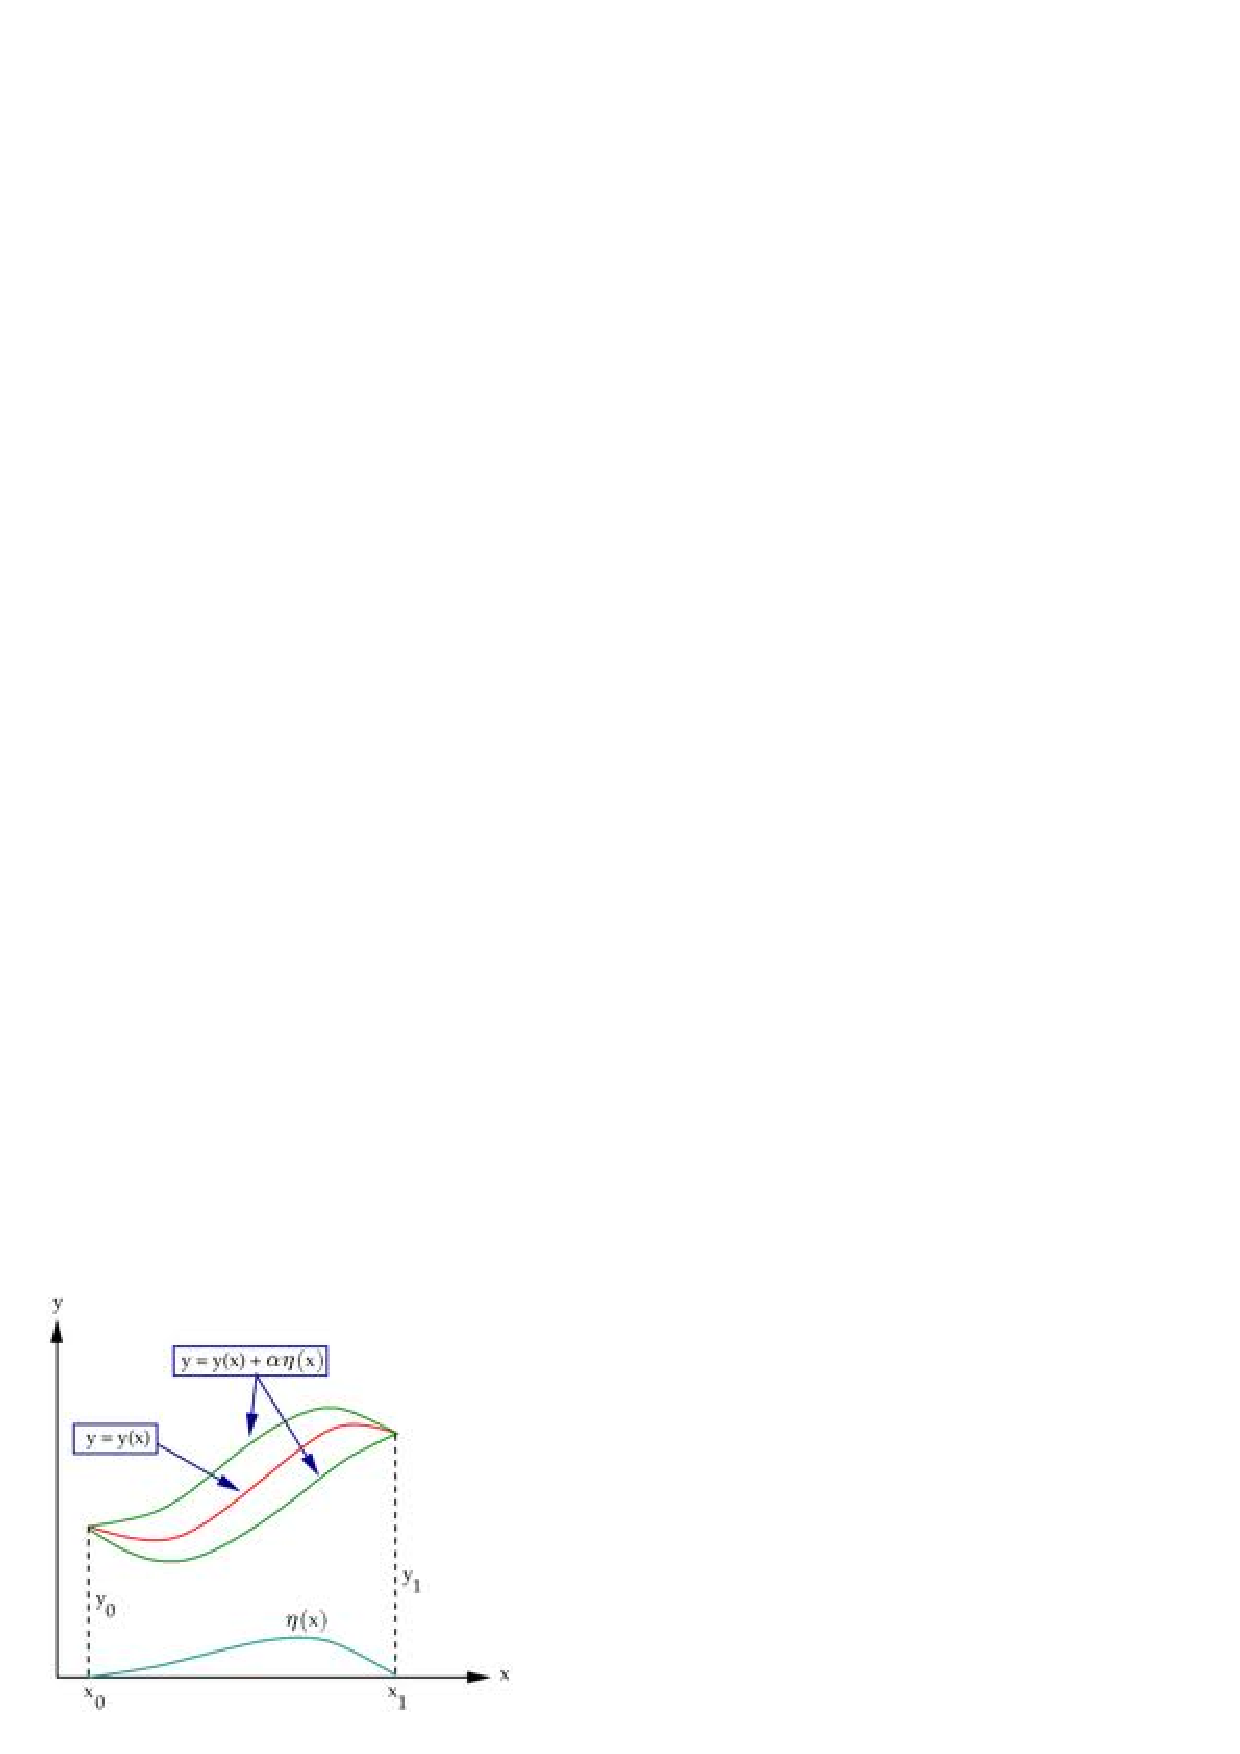
\includegraphics[width=0.3 \textwidth]{images.jpg}
\caption{variación infinitesimal de $y(x)$}
\label{lag}
\end{figure}
Donde $\alpha$ es un parámetro infinitesimal constante, $\eta(x)$ es una función \mbox{continua} y diferenciable que cumple con la condición de que se anula en los \mbox{extremos $\eta(x_1)=\eta(x_2)=0$,} lo que asegura la condición de extremos fijos. 
\\

A continuación, en la funcional \eqref{funcional} se reemplaza la curva extremal $y(x)$ por la curva variada $\overline{y}(x)$: 
\begin{equation}
W[y(x)]=\int\limits_{x_1}^{x_2}dx\ Z[y(x),\dot y(x),x] \ \Longrightarrow \ W[\overline{y}(x)]=\int\limits_{x_1}^{x_2}dx\ Z[\overline{y}(x),\dot {\overline{y}}(x),x]
\label{var} 
\end{equation}
con:
\begin{equation}
\dot {\overline{y}}(x)=\dot y(x)+\alpha\dot \eta(x)
\label{cur} 
\end{equation}
La relación \eqref{var} tendrá un extremo cuando \mbox{$\alpha=0$,} es decir \mbox{$\overline{y}(x)=y(x)$;} para \mbox{que $W[\overline{y}(x)]$} cumpla esta condición se debe garantizar \cite{hamilton}:
\begin{equation}
\left . \frac{d\ W[\overline{y}(x)]}{d\alpha}\right |_{\alpha=0}=\int\limits_{x_1}^{x_2}dx\left.\left(\frac{\partial Z}{\partial \overline{y} }\frac{\partial \overline{y}}{\partial\alpha}+\frac{\partial Z}{\partial \dot {\overline{y}}}\ \frac{\partial \dot {\overline{y}}}{\partial \alpha}\right)\right |_{\alpha=0}=0
\label{der} 
\end{equation}
La variación de la funcional \eqref{funcional}, definida como la diferencia entre la funcional evaluada en las curvas variadas $\overline{y}(x)$ y la funcional evaluada en la curva \mbox{extremal $y(x)$,} es nula:
\begin{equation}
\delta W=W[\overline{y}(x)]-W[{y}(x)]=0
\label{vaf} 
\end{equation}
debido a que cualquier variación o desvío infinitesimal alrededor de un extremo es de segundo orden \cite{hamilton,funcional}.
\\

Dado que la variación en la curva $y(x)$ es de la forma:
\begin{equation}
\delta y(x)=\overline{y}(x)-y(x)=\alpha\eta(x)=\alpha\frac{\partial \overline{y}}{\partial\alpha}
\label{deltaa} 
\end{equation}
la condición para que las curvas tengan extremos fijos, es equivalente a:
\begin{equation}
\delta y(x_1)=\delta y(x_2)=0
\label{confron}
\end{equation}
Entonces, para encontrar la curva extremal, se aplica la \mbox{condición \eqref{vaf}} sujeta a las condiciones de frontera \eqref{confron}. Teniendo en cuenta que los extremos $t_1$ y $t_2$ son \mbox{fijos, $\delta$ actuara} sobre la funcional \eqref{funcional}, de la siguiente manera:
\begin{equation}
\delta W=\alpha\left . \frac{d\ W[\overline{y}(x)]}{d\alpha}\right |_{\alpha=0}=0 
\end{equation}
\begin{equation}
\delta W=\delta\int\limits_{x_1}^{x_2}dx\ Z[y(x),\dot y(x),x]=\int\limits_{x_1}^{x_2}dx\left(\frac{\partial Z}{\partial y}\delta y+\frac{\partial Z}{\partial \dot y}\delta \dot y\right)=0
\end{equation}
la variación $\delta$ actúa  sobre las curvas y no sobre el parámetro $x$, por lo tanto es posible mostrar que $\delta$ y $\frac{d}{dx}$ conmutan, es decir:
\begin{equation}
\frac{d}{dx}\delta y(x)=\frac{d}{dx}\overline{y}(x)-\frac{d}{dx}y(x)=\delta \frac{d}{dx}y(x)
\end{equation}
de esta manera:
\begin{equation}
\delta W=\int\limits_{x_1}^{x_2}dx\left[\frac{\partial Z}{\partial y}\delta y-\frac{d}{dx}\left( \frac{\partial Z}{\partial \dot y}\right)\delta y+\frac{d}{dx}\left(\frac{\partial Z}{\partial \dot y}\delta y\right)\right]
\end{equation}          
\begin{equation}
\delta W=\int\limits_{x_1}^{x_2}dx\left[\frac{\partial Z}{\partial y}-\frac{d}{dx}\left( \frac{\partial Z}{\partial \dot y}\right)\right]\delta y+\left.\frac{\partial Z}{\partial \dot y}\delta y\right|_{x_1}^{x_2}
\end{equation}
de las condiciones de frontera \eqref{confron}, la variación de la funcional tiene la forma:
\begin{equation}
\delta W=\int\limits_{x_1}^{x_2}dx\left[\frac{\partial Z}{\partial y}-\frac{d}{dx}\left( \frac{\partial Z}{\partial \dot y}\right)\right]\delta y=0
\label{lema}
\end{equation}
El lema fundamental del cálculo de variaciones \cite{hamilton,ecudif}; establece que la condición para que \eqref{lema} sea valido es:
\begin{equation}
\frac{\partial Z}{\partial y}-\frac{d}{dx}\left( \frac{\partial Z}{\partial \dot y}\right)\ =\ 0
\label{lagrpsa} 
\end{equation}
La relación \eqref{lagrpsa} es una ecuación diferencial de segundo orden conocida como ecuación de Euler-Lagrange. La solución de esta ecuación diferencial sujeta a las condiciones de frontera $y(x_1)=y_1$ y $y(x_2)=y_2$; o $y(x_1)=y_1$ y $\dot y(x_1)=\dot y_1$, es la curva que extremiza la \mbox{funcional $W[y(x)]$.}
\subsection{Derivada funcional}
La funcional $W[y(x)]$ definida de la forma:
\begin{equation}
W[y(x)]=\int\limits_{x_1}^{x_2}dx\ Z[y(x),x]
\label{cero}
\end{equation} 
en donde $Z$ es función del parámetro $x$ y la curva $y(x)$, permite definir la variación de la funcional dada por \eqref{cero} en términos de la derivada funcional $\frac{\delta W}{\delta y(x)}$:   
\begin{equation}
\delta W[y(x)]=W[y(x)+\delta y(x)]-W[y(x)]=\int\limits_{x_1}^{x_2}dx\frac{\delta  W[y(x)] }{\delta y(x)}\delta y(x) 
\label{varfun}
\end{equation}
La derivada funcional calcula el cambio en $W[y(x)]$ cuando se realiza una variación infinitesimal de la curva $y(x)$ en el punto $x$, de manera que la variación total \mbox{de $W[y(x)]$} es una superposición lineal de las variaciones de $y(x)$ sumada sobre todos los valores de $x$ entre $[x_1,x_2]$. Si se construye una variación de la curva $y(x)$ en el punto $X$, en la forma de una distribución delta de Dirac \cite{greiner,funcional}:
\begin{equation}
\delta y(x)=\alpha\delta(x-X)
\label{deltd}
\end{equation}
donde $X\in[x_1,x_2]$ y $\alpha$ es un parámetro constante infinitesimal, se obtiene:
{\small
\begin{equation}
\delta W=W[y(x)+\alpha\delta(x-X)]-W[y(x)]=\int\limits_{x_1}^{x_2}dx\frac{\delta  W[y(x)] }{\delta y(x)}\alpha\delta(x-X)=\alpha\frac{\delta  W[y(x)] }{\delta y(X)}
\end{equation}}\\
lo que permite definir la derivada funcional de la siguiente manera:
\begin{equation}
\frac{\delta  W[y(x)]}{\delta y(X)}=\underset{\alpha\rightarrow0}{Lim}\ \frac{W[y(x)+\alpha\delta(x-X)]-W[y(x)]}{\alpha}  
\label{defu}
\end{equation}
La mayor parte de las reglas del cálculo diferencial ordinario también se aplican al cálculo funcional, algunas propiedades básicas de la derivada funcional son \cite{greiner, funcional}:
\begin{enumerate}
\item[\fbox{1.}] si $W[G[y(x)]]$ es una funcional de una funcional:
\begin{equation}
\frac{\delta W[G[y(x)]]}{\delta y(X)}=\frac{\delta  W[G[y(x)]]}{\delta G[y(x)]}\frac{\delta G[y(x)]}{\delta y(X)} 
\end{equation}
\item[\fbox{2.}] si $W[y(x)]=y(x)$
\begin{equation}
\frac{\delta y(x)}{\delta y(X)}=\delta(x-X) 
\end{equation}
\item[\fbox{3.}] si $W[y(x)]=\dot y(x)$
\begin{equation}
\frac{\delta\dot y(x)}{\delta y(X)}=\frac{d }{d x} \frac{\delta y(x)}{\delta y(X)}=\frac{d }{d x}\delta(x-X)=-\frac{d }{d X}\delta(x-X) 
\end{equation}
\item[\fbox{4.}] si $W[y(x)]=\int\limits_{x_1}^{x_2}dx\ Z[y(x),x]$
\begin{equation}
\frac{\delta W[y(x)]}{\delta y(X)}=\frac{d Z}{d y(x) } 
\end{equation}
\end{enumerate}
La condición para encontrar la curva extremal de la funcional \eqref{funcional} es equivalente a que su derivada funcional sea nula \cite{funcional}, de manera que se debe cumplir:
\begin{equation}
\frac{\delta W[y(x)]}{\delta y(X)}=0
\label{derfun}
\end{equation}
de acuerdo a la condición \eqref{derfun}, se determina que:
\begin{equation}
\frac{\delta W[y(x)]}{\delta y(X)}=\frac{\delta }{\delta y(X)}\int\limits_{x_1}^{x_2}dx\ Z[y(x),\dot y(x),x]=\int\limits_{x_1}^{x_2}dx\frac{\delta }{\delta y(X)} Z[y(x),\dot y(x),x] 
\end{equation}
\begin{equation}
=\int\limits_{x_1}^{x_2}dx\left(\frac{\partial \ Z}{\partial y}\frac{\delta y(x)}{\delta y(X)}+\frac{\partial \ Z}{\partial \dot y}\frac{\delta \dot y(x)}{\delta y(X)}  \right) 
\end{equation}
\begin{equation}
=\int\limits_{x_1}^{x_2}dx\left(\frac{\partial \ Z}{\partial y}\delta(x-X)-\frac{\partial \ Z}{\partial \dot y}\frac{d }{d X}\delta(x-X)\right) 
\end{equation}
\begin{equation}
=\int\limits_{x_1}^{x_2}dx\frac{\partial \ Z}{\partial y}\delta(x-X)-\frac{d }{d X}\int\limits_{x_1}^{x_2}dx\frac{\partial \ Z}{\partial \dot y}\delta(x-X) 
\end{equation}
\begin{equation}
\frac{\delta W[y(x)]}{\delta y(X)}=\frac{\partial \ Z}{\partial y(X)}-\frac{d }{d X}\frac{\partial \ Z}{\partial \dot y(X)}=0 
\end{equation}
Así, la curva que torna extremal la funcional \eqref{funcional} debe ser solución de las ecuaciones de Euler-Lagrange: 
\begin{equation}
\frac{\partial Z}{\partial y}-\frac{d}{dx}\left( \frac{\partial Z}{\partial \dot y}\right)\ =\ 0 
\label{eula}
\end{equation}
Para determinar si la curva es un máximo, mínimo o una inflexión, se utiliza el criterio de la segunda variación \cite{funcional}:
\begin{equation}
\delta^2 W[y_0(x)]\left\{ \begin{array}{lcl}
<0 & \mbox{máximo }\\
&
&
\\
=0 & \mbox{inflexión } 
&
\\
\\
>0 & \mbox{mínimo } 

\end{array}
\right.
\end{equation}
la segunda variación es definida de la forma \cite{funcional}:
{\small
\begin{equation}
\delta^2 W[y_0]= \frac{1}{2}\int\limits_{x_1}^{x_2}dX\int\limits_{x_1}^{x_2}dX'\left[\ y(X)-y_0(X)\ \right]\left[\ y(X')-y_0(X') \right]\left.\frac{\delta^2 W[y(x)] }{\delta y(X)\delta y (X')}\right|_{y_0}
\end{equation}}\\
Donde $y_0(x)$ es la solución de las ecuaciones de Euler-Lagrange y el ultimo término representa la segunda deriva funcional de $W[y(x)]$ evaluada en $y_0(x)$. De esta manera se determina si la curva $y_0(x)$ maximiza, minimiza o inflexiona la \mbox{funcional \eqref{funcional}.}    
\subsection{Principio de Fermat}
El principio de Fermat es la base teórica de la óptica geométrica \cite{ecudif,fin2,feyman}; formulado en 1662 es \mbox{fundamental} en el desarrollo del cálculo diferencial, el cálculo de variaciones y el principio de Hamilton. Fermat modifico el principio de distancia mínima de Herón de Alejandría, por el de tiempo mínimo \cite{ecudif,fin2,feyman}:
\\

\begin{center}
\fbox{ \parbox{0.9\linewidth}{\textit{El camino óptico que sigue un rayo de luz es aquel que minimiza el tiempo de trayectoria.}}}
\end{center}
De esta manera se deduce las leyes de Snell de la óptica geométrica. Si \mbox{consideramos} un rayo de luz que viaja del punto $S$ al punto $P$ pasando por una superficie $S$ que separa dos medios con diferentes índices de refracción (figura \ref{fermat}):
\begin{figure}[H]
\centering
\includegraphics[width=0.3 \textwidth]{snell.jpg}
\caption{refracción de un rayo de luz}
\label{fermat}
\end{figure} 
El tiempo total de recorrido es:
\begin{equation}
t=\frac{\sqrt{h^2+x^2}}{v_1}+\frac{\sqrt{b^2+(a-x)^2}}{v_2} 
\end{equation}
la condición de tiempo mínimo se cumple cuando:
\begin{equation}
\frac{dt}{dx}=\frac{x}{v_1\sqrt{h^2+x^2}}-\frac{(a-x)}{v_2\sqrt{b^2+(a-x)^2}}=0\ \ \ \ \ \ \ \ \ \ \ \frac{\sen \theta_1}{v_1}=\frac{sen \theta_2}{v_2}
\end{equation}
que es la ley de Snell, la cual fue deducida experimentalmente.
\\

El principio de Fermat también resuelve el problema de la \mbox{braquistócrona \cite{ecudif}}, de manera que este principio es fundamental en el desarrollo del principio de Hamilton.
\subsection{Sistemas físicos con un número finito de grados de libertad}
En mecánica clásica un sistema físico es descrito por un conjunto de $N$ coordenadas generalizadas o grados de libertad parametrizadas por el tiempo y denotadas en la forma $q_i(t)$, con $i=1,2...,N$; estos sistemas físicos se consideran que tienen un número finito de grados de libertad. A partir de estas coordenadas generalizadas, se asocia a un sistema físico conservativo una función denominada Langrangiano, esta cantidad definida como la diferencia entre la energía cinética y potencial es expresada en términos de las coordenadas generalizadas y describe completamente la dinámica del sistema físico \cite{hamilton}.
\\

Consideremos un sistema físico descrito por un Lagrangiano de orden $m$ en la derivadas, es decir:
\begin{equation}
L=L[\ q_i(t),\dot q_i(t),\ddot q_i(t),\dotso,\overset{m}{q}_i(t),t \ ]
\label{lagram}
\end{equation}
donde $L$, es función del tiempo, las coordenadas generalizadas y derivadas de \mbox{orden $m$} en las coordenadas generalizadas:
\begin{equation}
\overset{m}{q}_i(t)\equiv{ d^m\over dt^m }q_i(t) 
\end{equation}
Definido el Lagrangiano, se construye la funcional de acción entre los tiempos $[t_1,t_2]$:
\begin{equation}
A[q_i(t)]=\int\limits_{t_1}^{t_2}dtL[\ q_i(t),\dot q_i(t),\ddot q_i(t),\dotso,\overset{m}{q}_i(t),t \ ]
\label{acc} 
\end{equation}
Para deducir las ecuaciones de movimiento que gobiernan la evolución temporal del sistema físico aplicamos el principio de Hamilton \cite{hamilton,feyman2}:
\\
\begin{center}
\fbox{ \parbox{0.9\linewidth}{\textit{La trayectoria que sigue un sistema físico con un número finito de grados de libertad en el espacio de configuraciones entre los tiempos $[t_1,t_2]$, es aquella que hace extremal la funcional de acción:
\begin{equation}
\delta A[q_i(t)]=0 
\label{varacc}
\end{equation}}}}
\end{center}
la condición de acción extremal se debe cumplir teniendo en cuenta la siguientes condiciones de frontera:
\begin{equation}
\delta\ \overset{_{l-1}}{q}_i(t_1)=\delta \ \overset{_{l-1}}{q}_i(t_2)=0 
\label{fronfi}
\end{equation}
donde $l=1,2,...,m$ y $\overset{0}{q}_i(t)=q_i(t)$. De manera que si \mbox{$m=2$}, \mbox{$l=1,2$}; y por lo tanto las condiciones de frontera son:
\begin{equation}
\delta {q}_i(t_1) =\delta {q}_i(t_2)=0 \ \ \ \ \ \ \ \ \delta \dot{q}_i(t_1) =\delta \dot{q}_i(t_2)=0
\end{equation}
El principio de Hamilton es de tipo variacional y considera pequeñas variaciones de la trayectoria real:
\begin{equation}
\overline{q_i}(t)=q_i(t)+\delta q_i(t) 
\end{equation}
de manera que se debe aplicar las técnicas del cálculo de variaciones para determinar las ecuaciones de movimiento del sistema físico.
\\

El espacio de configuraciones esta conformado por la coordenadas \mbox{generalizadas $q_i(t)$} y sus derivadas $\overset{_{m}}{q}_i(t)$, las que se considera como un conjunto de coordenadas linealmente independientes que determinan la evolución temporal del sistema físico. La dimensión del espacio de configuraciones es $N(m+1)$ y tiene la forma:
\begin{equation}
(q_i,\dot q_i,\ddot q_i,....,\overset{_{m}}{q}_i) 
\end{equation}
Bajo el concepto de derivada funcional, la condición de acción extremal implica \mbox{que, (ver Eq \eqref{derfun}):}
\begin{equation}
\frac{\delta A[q_i(t)]}{\delta q_j(\tau)}=0 
\end{equation}
Utilizando las siguientes propiedades básicas de derivada funcional \cite{funcional}: 
\begin{equation}
\frac{\delta q_i(t)}{\delta q_j(\tau)}=\delta_{ij} \delta(t-\tau)\ \ \ \ \ \frac{\delta [\overset{m}{q}_i(t)]}{\delta {q}_j(\tau)}=\delta_{ij} \frac{d^m}{dt^m}\delta(t-\tau)=(-1)^m\delta_{ij} \frac{d^m}{d\tau^m}\delta(t-\tau) 
\label{propfun}
\end{equation}
se deducen las ecuaciones de movimiento de \mbox{Euler-Lagrange} que determinan la evolución temporal en el espacio de configuraciones para un sistema físico que posee un número finito de grados de libertad y que es descrito por Lagrangianos de \mbox{orden $m$} en las derivadas, (\mbox{ver Apéndice A):} 
\begin{equation}
\frac{\delta A[q_i(t)]}{\delta q_j(\tau)}=\frac{\partial L}{\partial q_i} \ -\  \frac{d}{dt}\left(\frac{\partial L}{\partial \dot q_i}\right)+\frac{d^2}{dt^2}\left(\frac{\partial L}{\partial \ddot q_i}\right)+\dotso+(-1)^m\frac{d^m}{dt^m}\left(\frac{\partial L}{\partial (\overset{m}{q}_i)}\right)=0  
\end{equation}
Este resultado puede ser generalizado de la forma:
\begin{equation}
\sum\limits_{k=o}^m(-1)^k\frac{d^k}{dt^k}\left(\frac{\partial L}{\partial(\overset{k}{q}_i )} \right)\ =\ 0 
\end{equation}
Las ecuaciones de movimento de Euler-Lagrange es un conjunto de $N$ ecuaciones diferenciales de orden $2m$ en las derivadas temporales. Así, para garantizar unicidad en la solución se requieren $2Nm$ condiciones iniciales.
\subsection{Sistemas físicos con un número infinito de grados de libertad}
En teoría clásica de campos \cite{noether}, los sistemas físicos son representados por campos que están definidos en el espacio-tiempo. De esta manera, sistemas físicos tales como el campo electromagnético, campos escalares, campos de Dirac, etc; son \mbox{representados} en el espacio de Minkowski en la forma $\psi_a(x)$, donde  $a=1,..,N$; es el número de componentes o grados de libertad y \mbox{$x=x^\mu=(x^0,x^1,x^2,x^3)$ } \mbox{con $\mu=0,1,2,3$;} \mbox{denota} un evento o un punto en el \mbox{espacio-tiempo \cite{greiner}.} A cada evento del \mbox{espacio-tiempo} le corresponde un valor de campo y como la estructura del espacio-tiempo es continua, se considera que estos sistemas físicos poseen un número infinito de grados de libertad. Definidos los campos, se le asocia al sistema físico una densidad Lagrangiana $\mathscr{L}$ la cual describirá la dinámica y las propiedades del sistema físico y cumple la característica de ser un escalar o invariante de \mbox{Lorentz \cite{greiner}.} Consideremos un sistema físico descrito por una densidad Lagrangiana de orden $m$ en la derivadas:
\begin{equation}
\mathscr{L}[\psi_a(x),\partial_{\mu_1}\psi_a(x),\partial_{\mu_1}\partial_{\mu_2}\psi_a(x),\dotso,\partial_{\mu_1}\partial_{\mu_2}\dotso\partial_{\mu_m}\psi_a(x),x]
\label{lanorm}
\end{equation}
donde $\partial_{\mu}$ es la derivada covariante en el espacio de Minkowski:
\begin{equation}
\partial_{\mu}=(\partial_0,\partial_1,\partial_2,\partial_3)=\left(\frac{\partial}{\partial x^0},\frac{\partial}{\partial x^1},\frac{\partial}{\partial x^2},\frac{\partial}{\partial x^3} \right) 
\end{equation}
y:
\begin{equation}
\partial_{\mu_1}\partial_{\mu_2}\dotso\partial_{\mu_m}=\frac{\partial^m}{\partial x_1^\mu\partial x_2^\mu...\partial x_m^\mu} 
\end{equation}

El Lagrangiano asociado al campo definido sobre una región $\Omega$ del espacio es definido por:
\begin{equation}
L=\int\limits_{\Omega}d^3 x \mathscr{L}
\end{equation}
con $dx^3=dx^1dx^2dx^3$. La funcional de acción entre los tiempos $t_1$ y $t_2$ es construida a partir del Lagrangiano en la forma \cite{noether, greiner}:
\begin{equation}
A[\psi_a(x)]=\int\limits_{t_1}^{t_2}dtL=\int\limits_{t_1}^{t_2}dt\int\limits_{\Omega}d^3 x \mathscr{L}=\int\limits_{\sigma}d^4x \mathscr{L}
\label{acmos}
\end{equation}
donde $\sigma$ es el volumen en el espacio-tiempo y \mbox{$dx^4=dx^0dx^1dx^2dx^3$}
\\

Para \mbox{deducir} las \mbox{ecuaciones} de movimiento para sistemas físicos descritos por campos de la forma \mbox{$\psi_a(x)=\psi_a(\textbf{x},t)$} con $\textbf{x}=(x^1,x^2,x^3)$; utilizamos el principio de \mbox{Hamilton \cite{noether, greiner}:}
\begin{center}
\fbox{ \parbox{0.9\linewidth}{\textit{La trayectoria que sigue un sistema físico representado por campos, en el \mbox{espacio} de \mbox{configuraciones} entre los tiempos $[t_1,t_2]$, es aquella que hace extremal la funcional de acción:
\begin{equation}
\delta A[\psi_a(x)]=0 
\label{hacam}
\end{equation}
}}}
\end{center}
la condición de acción extremal se debe cumplir bajo las condiciones de frontera:
\begin{eqnarray}
\delta \psi_a(\textbf{x},t_1)=\delta \psi_a(\textbf{x},t_2)=0   \\
\label{fronterascam}
\delta \dot \psi_a(\textbf{x},t_1)=\delta\dot  \psi_a(\textbf{x},t_2)=0 \nonumber \\
\delta \ddot \psi_a(\textbf{x},t_1)=\delta\ddot  \psi_a(\textbf{x},t_2)=0\nonumber \\
\vdots\nonumber \\
\delta \overset{_{m-1}}\psi_a(\textbf{x},t_1)=\delta\overset{_{m-1}}\psi_a(\textbf{x},t_2)=0 \nonumber
\end{eqnarray}
junto a las condiciones asintóticas en los campos:
\begin{equation}
|\textbf{x}|\rightarrow\infty \ \ \ \left\{ \begin{array}{lcl}
\psi_a(\textbf{x},t)\rightarrow0 \\
\dot \psi_a(\textbf{x},t)\rightarrow0 \\
\ddot \psi_a(\textbf{x},t)\rightarrow0\\
\vdots \\
\overset{_{m-1}}{\psi}_a(\textbf{x},t)\rightarrow0 
\label{sinto}
\end{array}
\right.
\end{equation}
el principio de Hamilton considera variaciones infinitesimales con respecto a la trayectoria real, de manera que se debe aplicar las técnicas del cálculo de variaciones para determinar las ecuaciones de movimiento de un sistema físico.
\\

El espacio de configuraciones esta constituido por los campos $\psi_a(x)$ y sus derivadas temporales $\overset{_{m}}\psi_a(x)$, así, el espacio de configuraciones tendrá la estructura:
\begin{equation}
(\psi_a,\dot \psi_a,\ddot \psi_a,\dotso,\overset{_{m}}{\psi}_a) 
\end{equation}
donde \mbox{$\overset{_{m}}{\psi}_a=\partial_0^m{\psi}_a$}. El espacio de configuraciones es un conjunto de \mbox{variables} \mbox{linealmente} independientes y su dimensión \mbox{es $N(m+1)$.}
\\

La condición de acción extremal, es garantizada si \cite{noether}:
\begin{equation}
\frac{\delta A[\psi_a(x)]}{\delta \psi_b(y)}=0 
\label{funcam}
\end{equation}
De la condición \eqref{funcam}, es posible determinar las ecuaciones de movimiento de \mbox{Euler-Lagrange}, mejor conocidas como ecuaciones de campo. El comportamiento dinámico del sistema físico descrito por $\psi_a(x)$, esta dado por, (ver Apéndice B):
\begin{equation}
\frac{\partial\mathscr{L} }{\partial \psi_a}-\partial_{\mu_1}\left(\frac{\partial \mathscr{L}}{\partial(\partial _{\mu_1}\psi_a)}\right)+...+(-1)^m\partial_{\mu_1}\partial_{\mu_2}...\partial_{\mu_m}\left(\frac{\partial \mathscr{L}}{\partial (\partial_{\mu_1}\partial_{\mu_2}...\partial_{\mu_m}\psi_a)}\right)=0 
\label{euge}
\end{equation}
Esta ecuación puede ser escrita de forma compacta de la siguiente manera \cite{general}:
\begin{equation}
\sum\limits_{i=o}^m(-1)^i\prod\limits_{j=o}^i\partial_{\mu_j}\left(\frac{\partial\mathscr{L} }{\partial(\prod\limits_{j=o}^i\partial_{\mu_j}\psi_a)} \right)\ =\ 0 
\end{equation}
con \mbox{$\partial_{\mu_0}=1$} y \mbox{$a=1,2,\dotso,N$}; es el número de grados de libertad.
\newpage 
\section{Leyes de conservación en teoría clásica de campos}
Noether en el año de 1918 en su artículo  \textit{``Invariante variationsprobleme''} formaliza las leyes de conservación. Noether al imponer la condición que la acción debe ser invariante por transformaciones de coordenadas y campos, obtiene una relación entre las simetrías en las leyes de la física y las cantidades \mbox{conservadas \cite{ noether, greiner, emmy}}. El teorema de Noether que en este capitulo se desarrollara para sistemas físicos descritos por Lagrangianos de orden $m$ en las derivadas \cite{general}, tiene dos partes:
\\

El primer teorema de Noether establece que la invariancia del Lagrangiano ante un grupo de simetría finito o global, implica la existencia de cantidades \mbox{conservadas}, de esta manera como consecuencia del grupo de simetría global de Poincaré, se obtiene expresiones para la energía, el momentum lineal, el momentum \mbox{angular} y el spin, demostrando que estas cantidades son \mbox{conservadas \cite{ noether, greiner, emmy}}. Del cálculo de la energía se deduce una expresión \mbox{generalizada} para el Hamiltoniano canónico y los momentos canónicos asociados a cada uno de los campos linealmente \mbox{independientes}, lo que permite desarrollar una versión canónica de este tipo de \mbox{teorías \cite{general}.}
\\

El segundo teorema de Noether, establece que la invariancia del Lagrangiano ante un grupo de simetría infinito, es decir simetrías de gauge locales, implica: la existencia de cantidades conservadas, el cumplimiento de las identidades de Bianchi, y un Lagrangiano singular, resultado en sistemas dinámicos con vínculos \cite{noether,emmy,local}. Dirac estableció el método para el estudio canónico de estos sistemas, método que es fundamental en la cuantización de este tipo de \mbox{teorías \cite{dirac, canoalor}.}
\subsection{Teorema de Noether}
Las leyes de conservación en física, son cantidades que permanecen constantes en el tiempo independiente de la evolución dinámica de un sistema físico y son \mbox{consecuencia} de simetrías en la leyes de la física, es decir de la invariancia del \mbox{Lagrangiano} ante transformaciones de coordenadas y campos pertenecientes a un determinado grupo de simetría \cite{ noether, greiner, emmy}.
\\

Consideremos un sistema físico descrito por campos al cual se le asocia una densidad Lagrangiana de orden dos en las derivadas:
\begin{equation}
\mathscr{L}=\mathscr{L}[\psi_a(x),\partial_\mu\psi_a(x),\partial_\mu\partial_\nu\psi_a(x),x] 
\end{equation}
a partir del Lagrangiano se construye la funcional de acción:
\begin{equation}
A[\psi_a(x)]=\int\limits_{\sigma}d^4 x \mathscr{L}
\label{accod}
\end{equation}
Las leyes de conservación son consecuencia de la invariancia de la acción ante las siguientes transformaciones continuas de coordenadas y campos:
\begin{equation}
x^{'}=x^{'}(x) \ \ \ \ \ \ \ \ \ \psi_a^{'}(x^{'})=\psi_a^{'}[\psi_a(x)]
\end{equation}
las cuales pueden ser construidas a partir de transformaciones infinitesimales \cite{general, greiner}:
\begin{equation}
x^{'\mu}=x^{\mu}+\delta x^{\mu} \ \ \ \ \ \ \psi_a^{'}(x^{'})=\psi_a(x)+\delta\psi_a(x)
\label{traninfi}
\end{equation}
La variación local $\delta\psi_a(x)$, es consecuencia de la transformación de coordenadas y campos: 
\begin{equation}
\delta\psi_a(x)=\psi_a^{'}(x^{'})-\psi_a(x)=\psi_a^{'}(x+\delta x)-\psi_a(x)
\label{locglo}
\end{equation}
$$\approx\psi_a^{'}(x)+ \delta x^{\mu}\partial_\mu\psi_a(x)-\psi_a(x)=\overset{\_}{\delta}\psi_a(x)+\delta x^{\mu}\partial_\mu\psi_a(x)$$
en donde se hizo un expansión en series de Taylor para $\psi_a^{'}(x+\delta x)$ considerando términos de primer orden y se introdujo el concepto de variación global $\overset{\_}{\delta}\psi_a(x)$, que representa cambios solo en la forma de los campos, sin tener cambios en el punto $x$ del espacio-tiempo \cite{noether,general,greiner}:
\begin{equation}
\overset{\_}{\delta}\psi_a(x)=\psi_a^{'}(x)-\psi_a(x)
\label{globalvari}
\end{equation}
Debido a la definición \eqref{globalvari}, es posible mostrar que la variación global conmuta con las derivadas \cite{noether, greiner}:
\begin{equation}
\partial_{\mu}[\overset{\_}{\delta}\psi_a(x)]=\partial_{\mu}[\psi_a^{'}(x)-\psi_a(x)]=\partial_{\mu}[\psi_a^{'}(x)]-\partial_{\mu}[\psi_a(x)]=\overset{\_}{\delta}[\partial_{\mu}\psi_a(x)] 
\label{conglo}
\end{equation}
por el contrario la variación local no presenta esta característica, (ver \mbox{Apéndice C) \cite{noether,greiner}:}
\begin{equation}
\partial_{\mu}[\delta\psi_a(x)]\approx\delta[\partial_{\mu}\psi_a(x)]+[\partial_{\mu} \delta x^{\alpha}][\partial_{\alpha}\psi_a(x)]
\end{equation}
Como consecuencia de las transformaciones infinitesimales de coordenadas y campos dada por \eqref{traninfi}, la variación de la densidad Lagrangiana se expresa como:
\begin{equation}
\mathscr{L}^{'}=\mathscr{L}+\delta\mathscr{L}
\label{varlangr}
\end{equation}
donde:
\begin{equation}
\mathscr{L}^{'}=\mathscr{L}^{'}[\psi_a^{'}(x^{'}),\partial_{\mu}^{'}\psi_a^{'}(x^{'}),\partial_{\mu}^{'}\partial_{\nu}^{'}\psi_a^{'}(x^{'}),x^{'}] 
\end{equation}
Al exigir que la acción sea invariante por transformaciones infinitesimales de coordenadas y campos \eqref{traninfi}, se debe cumplir: \cite{general,noether,greiner}:
\begin{equation}
\delta A[\psi_a (x)]=A^{'}[\psi_a^{'}(x^{'})]-A[\psi_a(x)]=\int\limits_{\sigma^{'}}dx^{'4}\mathscr{L}^{'}-\int\limits_{\sigma}dx^4\mathscr{L}=0 
\label{acno} 
\end{equation}
donde $\sigma^{'}$ denota el volumen expresado en términos de las coordenadas $x^{'}$.
\\
  
La relación entre el elemento de volumen $dx^{4}$ y el volumen $dx^{'4}$ en las nuevas coordenadas, se determina a partir del Jacobiano de \mbox{transformación \cite{general, noether, greiner}}: 
\begin{equation}
dx^{'4}=\left|\frac{\partial x^{'\mu}}{\partial x^{\alpha}}\right|dx^{4}=\left|\frac{\partial }{\partial x^{\alpha}}(x^{\mu}+\delta x^{\mu})\right|dx^{4}=\left|\delta_{\ \alpha}^\mu+\partial_\alpha(\delta x^{\mu})\right|dx^{4} 
\end{equation}
teniendo en cuenta que las transformaciones de coordenadas son infinitesimales, se debe considerar términos de primer orden en el Jacobiano:
\begin{equation}
\left|\frac{\partial x^{'\mu}}{\partial x^{\alpha}}\right|=\left|\begin{matrix}
1+\partial_0 \delta x^{0} & \partial_1 \delta x^{0} & \partial_2 \delta x^{0} & \partial_3 \delta x^{0}\\
\\ \partial_0 \delta x^{1} & 1+\partial_1 \delta x^{1} & \partial_2 \delta x^{1} & \partial_3 \delta x^{1}\\
\\ \partial_0 \delta x^{2} & \partial_1 \delta x^{2} & 1+\partial_2 \delta x^{2} & \partial_3\delta x^{2}\\
\\ \partial_0 \delta x^{3} & \partial_1\delta x^{3} & \partial_2 \delta x^{3} & 1+\partial_3\delta x^{3}\\
\end{matrix}\right|\approx1+\partial_{\mu} \delta x^\mu  
\end{equation}
de esta manera, la relación entre los elementos de volumen $dx^{4}$ y $dx^{'4}$ es:
\begin{equation} 
dx^{'4}=(1+\partial_{\mu}\delta x^\mu)dx^{4} 
\label{jaco}
\end{equation}
Sustituyendo las relaciones \eqref{jaco} y \eqref{varlangr} en la \mbox{expresión \eqref{acno}} y considerando, nuevamente términos de primer orden, se obtiene: 
\begin{equation}
\delta A[\psi_a (x)]=\int\limits_{\sigma}dx^{4}(1+\partial_{\mu}\delta x^\mu)\left(\mathscr{L}+\delta \mathscr{L} \right)-\int\limits_{\sigma}dx^4\mathscr{L}=0 
\label{lolanglo}           
\end{equation}
$$
\approx\int\limits_{\sigma}dx^{4}[\delta\mathscr{L}+\mathscr{L}(\partial_{\mu}\delta x^\mu)]=0     
$$
expresando la variación local del Lagrangiano $\delta \mathscr{L}$, en términos de la variación global del mismo, $\overset{\_}{\delta}\mathscr{L}$, ecuación \eqref{locglo}:
\begin{equation}
\delta \mathscr{L}=\overset{\_}{\delta}\mathscr{L}+\delta x^{\mu}\partial_\mu\mathscr{L}
\end{equation}
la relación \eqref{lolanglo} puede ser escrita en la forma:
\begin{equation}
\delta A[\psi_a (x)]=\int\limits_{\sigma}dx^{4}[\overset{\_}{\delta}\mathscr{L}+\partial_{\mu}(\delta x^{\mu}\mathscr{L})]=0         
\label{actra}
\end{equation}
Se puede expresar la variación global del Lagrangiano en términos de las variaciones globales del campo y de sus derivadas de la siguiente manera: 
\begin{equation}
\overset{\_}{\delta}\mathscr{L}=\frac{\partial\mathscr{L} }{\partial \psi_a}\overset{\_}{\delta}\psi_a +\frac{\partial\mathscr{L} }{\partial(\partial_{\mu} \psi_a)}\overset{\_}{\delta}(\partial_{\mu} \psi_a)+\frac{\partial\mathscr{L} }{\partial(\partial_{\mu}\partial_{\nu} \psi_a)}\overset{\_}{\delta}(\partial_{\mu}\partial_{\nu} \psi_a)
\label{varlaglo} 
\end{equation}
teniendo en cuenta \eqref{conglo} y del hecho que $\partial_{\mu}\partial_{\nu} \overset{\_}{\delta}\psi_a=\partial_{\mu}\partial_{\nu}[\psi_a^{'}(x)-\psi_a(x)]=\overset{\_}{\delta}(\partial_{\mu}\partial_{\nu} \psi_a)$, la anterior ecuación se expresa en la forma: 
\begin{equation}
\overset{\_}{\delta}\mathscr{L}=\frac{\partial\mathscr{L} }{\partial \psi_a}\overset{\_}{\delta}\psi_a +\frac{\partial\mathscr{L} }{\partial(\partial_{\mu} \psi_a)}\partial_{\mu}(\overset{\_}{\delta} \psi_a)+\frac{\partial\mathscr{L} }{\partial(\partial_{\mu}\partial_{\nu} \psi_a)}\partial_{\mu}\partial_{\nu}(\overset{\_}{\delta} \psi_a)  
\label{varlas}
\end{equation}
Utilizando las siguientes relaciones:
\begin{equation}
\frac{\partial\mathscr{L} }{\partial(\partial_{\mu} \psi_a)}\partial_{\mu}(\overset{\_}{\delta} \psi_a)=\partial_{\mu}\left(\frac{\partial\mathscr{L} }{\partial(\partial_{\mu} \psi_a)}\overset{\_}{\delta} \psi_a\right)-\partial_{\mu}\left(\frac{\partial\mathscr{L} }{\partial(\partial_{\mu} \psi_a)}\right)\overset{\_}{\delta} \psi_a 
\end{equation}
$$
\frac{\partial\mathscr{L} }{\partial(\partial_{\mu}\partial_{\nu} \psi_a)}\partial_{\mu}\partial_{\nu}(\overset{\_}{\delta} \psi_a)=\partial_{\mu}\left(\frac{\partial\mathscr{L} }{\partial(\partial_{\mu}\partial_{\nu} \psi_a)}\partial_{\nu}\overset{\_}{\delta} \psi_a\right)-\partial_{\nu}\left[\partial_{\mu}\left(\frac{\partial\mathscr{L} }{\partial(\partial_{\mu}\partial_{\nu} \psi_a)}\right)\overset{\_}{\delta} \psi_a\right] 
$$
$$+\partial_{\nu}\partial_{\mu}\left(\frac{\partial\mathscr{L} }{\partial(\partial_{\mu}\partial_{\nu} \psi_a)}\right)\overset{\_}{\delta}\psi_a$$
la expresión \eqref{varlas}, se reescribe en la forma:
\begin{equation}
\overset{\_}{\delta}\mathscr{L}=\frac{\partial\mathscr{L} }{\partial \psi_a}\overset{\_}{\delta}\psi_a+\partial_{\mu}\left(\frac{\partial\mathscr{L} }{\partial(\partial_{\mu} \psi_a)}\overset{\_}{\delta} \psi_a\right)-\partial_{\mu}\left(\frac{\partial\mathscr{L} }{\partial(\partial_{\mu} \psi_a)}\right)\overset{\_}{\delta} \psi_a
\label{varlola}
\end{equation}
$$+\partial_{\mu}\left(\frac{\partial\mathscr{L} }{\partial(\partial_{\mu}\partial_{\nu} \psi_a)}\partial_{\nu}\overset{\_}{\delta} \psi_a\right)-\partial_{\nu}\left[\partial_{\mu}\left(\frac{\partial\mathscr{L} }{\partial(\partial_{\mu}\partial_{\nu} \psi_a)}\right)\overset{\_}{\delta} \psi_a\right]+\partial_{\nu}\partial_{\mu}\left(\frac{\partial\mathscr{L} }{\partial(\partial_{\mu}\partial_{\nu} \psi_a)}\right)\overset{\_}{\delta}\psi_a $$
Al sustituir \eqref{varlola} en \eqref{actra}, la invariancia de la acción ante transformaciones de coordenadas y campos implica:
\begin{equation}
\delta A[\psi_a (x)]=\int\limits_{\sigma}dx^{4}\left[\frac{\partial\mathscr{L} }{\partial \psi_a}-\partial_{\mu}\left(\frac{\partial\mathscr{L} }{\partial(\partial_{\mu} \psi_a)}\right)+\partial_{\mu}\partial_{\nu}\left(\frac{\partial\mathscr{L} }{\partial(\partial_{\mu}\partial_{\nu} \psi_a)}\right)\right]\overset{\_}{\delta}\psi_a
\label{canoe}
\end{equation}  
$$+\int\limits_{\sigma}dx^{4}\partial_{\mu}\left\{\left[\frac{\partial \mathscr{L} }{\partial(\partial_{\mu} \psi_a)}-\partial_{\nu}\left(\frac{\partial\mathscr{L} }{\partial(\partial_{\nu}\partial_{\mu} \psi_a)}  \right) \right]\overset{\_}{\delta}\psi_a\ +\ \frac{\partial\mathscr{L} }{\partial(\partial_{\mu}\partial_{\nu} \psi_a)}\partial_{\nu}\overset{\_}{\delta} \psi_a+\mathscr{L}\delta x^\mu \right\}=0$$
Denotando las ecuaciones de Euler-Lagrange para Lagrangianos de segundo orden de la siguiente manera:
\begin{equation}
L^a=\frac{\partial\mathscr{L} }{\partial \psi_a}-\partial_{\mu}\left(\frac{\partial\mathscr{L} }{\partial(\partial_{\mu} \psi_a)}\right)+\partial_{\mu}\partial_{\nu}\left(\frac{\partial\mathscr{L} }{\partial(\partial_{\mu}\partial_{\nu} \psi_a)}\right)=0
\label{la}
\end{equation}
y definiendo la corriente de Noether, de la forma:
\begin{equation}
J^\mu=\left[\frac{\partial \mathscr{L} }{\partial(\partial_{\mu} \psi_a)}-\partial_{\nu}\left(\frac{\partial\mathscr{L} }{\partial(\partial_{\nu}\partial_{\mu} \psi_a)}  \right) \right]\overset{\_}{\delta}\psi_a\ +\ \frac{\partial\mathscr{L} }{\partial(\partial_{\mu}\partial_{\nu} \psi_a)}\partial_{\nu}\overset{\_}{\delta} \psi_a\ \ + \ \mathscr{L}\delta x^\mu
\label{corr}
\end{equation}
la ecuación \eqref{canoe} se escribe como:
\begin{equation}
\delta A[\psi_a (x)]=\int\limits_{\sigma}dx^{4}\left(L^a\overset{\_}{\delta}\psi_a+\partial_\mu J^\mu \right)=0 
\label{voar}
\end{equation}
Teniendo en cuenta que el volumen en el espacio-tiempo $\sigma$ es arbitrario y que la identidad \eqref{voar} se debe garantizar independientemente de $\sigma$, la condición de invariancia de la acción ante transformaciones infinitesimales de coordenadas y campos implica \cite{noether,general,greiner}:
\begin{equation}
L^a\overset{\_}{\delta}\psi_a+\partial_\mu J^\mu=0 
\label{noeemy}
\end{equation}
la expresión \eqref{noeemy}, es conocido como el teorema de Noether. 
\subsection{Primer teorema de Noether}
Si las variaciones en coordenadas y campos: $\delta x^{\mu}$, $\delta\psi_a$; están caracterizadas por un conjunto infinitesimal de $r$ parámetros constantes e independientes del \mbox{espacio-tiempo} $\in^\beta $, con $\beta=1,2,..r$; el conjunto de transformaciones pertenecen a un grupo de simetría finito \cite{ noether, greiner, emmy}: 
\begin{equation}
\delta x^{\mu}=x^{'\mu}-x^{\mu}=\in^\beta X_{\ \beta}^\mu(x)
\label{glocon}
\end{equation}
$$\delta\psi_a(x)=\psi_a^{'}(x^{'})-\psi_a(x)=\in^\beta \Phi_{\beta a}(x)$$
donde $X_{\ \beta}^\mu(x)$ y $\Phi_{\beta a(x)}$ son los generadores del grupo de simetría. Los generadores pertenecen a un mínimo subgrupo del grupo de transformaciones, de manera que todo elemento del grupo de simetría puede ser expresado en términos de los generadores del grupo.
\\

Si se considera invariancia de la acción ante un grupo de simetría finito, junto a la condición que el sistema físico descrito por campos $\psi_a(x)$ satisface las ecuaciones de \mbox{Euler-Lagrange,} es decir \mbox{$L^a=0$}, el primer teorema de Noether establece la siguiente ecuación de \mbox{continuidad \cite{noether,general,greiner}:}
\begin{equation}
\partial_\mu J^\mu=0 
\label{nocopr}
\end{equation}
donde $J^\mu$, se define como la corriente de Noether, que expresada en función de variaciones locales se escribe como: 
\begin{equation}
J^\mu=\left[\frac{\partial \mathscr{L} }{\partial(\partial_{\mu} \psi_a)}-\partial_{\nu}\left(\frac{\partial\mathscr{L} }{\partial(\partial_{\nu}\partial_{\mu} \psi_a)}  \right) \right]\delta\psi_a\ +\ \frac{\partial\mathscr{L} }{\partial(\partial_{\mu}\partial_{\nu} \psi_a)}\delta\partial_\nu\psi_a
\label{corrino}
\end{equation}
$$ -\delta x^\alpha\left\{\ \ \ \left[\frac{\partial \mathscr{L} }{\partial(\partial_{\mu} \psi_a)}-\partial_{\nu}\left(\frac{\partial\mathscr{L} }{\partial(\partial_{\nu}\partial_{\mu} \psi_a)}  \right) \right]\partial_\alpha\psi_a +\ \frac{\partial\mathscr{L} }{\partial(\partial_{\mu}\partial_{\nu} \psi_a)}\partial_\alpha\partial_\nu\psi_a-\delta^\mu_{\ \alpha}\mathscr{L}   \right\}$$
Considerando un grupo de simetría finito \eqref{glocon} y el hecho que los parámetros $\in^\beta$ son constantes, la ecuación de continuidad \eqref{nocopr} es reescrita de la forma:
\begin{equation}
\in^\beta\partial_\mu J^\mu_{\ \beta}=\partial_\mu J^\mu_{\ \beta}=0 
\label{congene}
\end{equation}
donde $J^\mu_{\ \beta}$, es la corriente de Noether expresada en función de los generadores del grupo de simetría finito:
\begin{equation}
J^\mu_{\ \beta}=\left[\frac{\partial \mathscr{L} }{\partial(\partial_{\mu} \psi_a)}-\partial_{\nu}\left(\frac{\partial\mathscr{L} }{\partial(\partial_{\nu}\partial_{\mu} \psi_a)}  \right) \right]\Phi_{\beta a}(x)+\frac{\partial\mathscr{L} }{\partial(\partial_{\mu}\partial_{\nu} \psi_a)}\partial_\nu\Phi_{\beta a}(x)
\label{corrinoss}
\end{equation}
$$ -X_{\ \beta}^\alpha(x)\left\{\ \ \ \left[\frac{\partial \mathscr{L} }{\partial(\partial_{\mu} \psi_a)}-\partial_{\nu}\left(\frac{\partial\mathscr{L} }{\partial(\partial_{\nu}\partial_{\mu} \psi_a)}  \right) \right]\partial_\alpha\psi_a +\ \frac{\partial\mathscr{L} }{\partial(\partial_{\mu}\partial_{\nu} \psi_a)}\partial_\alpha\partial_\nu\psi_a-\delta^\mu_{\ \alpha}\mathscr{L}   \right\}$$
\\

Integrando en el espacio la ecuación de continuidad \eqref{congene}:
\begin{equation}
\int\limits_{\Omega}dx^{3}\partial_\mu J^\mu_{\ \beta}=\int\limits_{\Omega}dx^{3}(\partial_0 J^0_{\ \beta}+\partial_k J^k_{\ \beta})=0 
\label{gauus}
\end{equation}
al utilizar el teorema de Gauus, el término:
\begin{equation}
\int\limits_{\Omega}dx^{3}(\partial_k J^k_{\ \beta})=\oint\limits_{s}d_{s_k}J^k_{\ \beta}
\end{equation}
siendo $s$ la superficie cerrada que es contorno del volumen $\Omega$. El volumen de integración $\Omega$ es arbitrario, y lo podemos escoger tan grande como se deseé, al considerar campos completamente asintóticos, es decir:
\begin{equation}
\left.\begin{array}{lcl}
\psi_a(\textbf{x},t)\rightarrow0 \\
\partial_k \psi_a(\textbf{x},t)\rightarrow0 \\
\end{array}
\right\} \mbox{cuando}\ |\textbf{x}|\rightarrow\infty
\label{asindos}
\end{equation}
se obtiene, que cuando $|\textbf{x}|\rightarrow\infty$:
\begin{equation}
\int\limits_{\Omega}dx^{3}(\partial_k J^k_{\ \beta})=\oint\limits_{s}d_{s_k}J^k_{\ \beta}\rightarrow0  
\end{equation}
por lo tanto, \eqref{gauus} se expresa como:
\begin{equation}
\int\limits_{\Omega}dx^{3}\partial_0 J^0_{\ \beta}=\frac{d}{dt}\int\limits_{\Omega}dx^{3}J^0_{\ \beta}=\frac{d}{dt}Q_{\beta}= 0 
\end{equation}
la cantidad:
\begin{equation}
Q_{\beta}=\int\limits_{\Omega}dx^{3}J^0_{\ \beta}=\mbox{constante} \ \ \ \ \beta=1,2,..,r
\label{carnoem}
\end{equation}
se denomina carga de Noether.
\\

La ecuación de continuidad establece la existencia de $r$ cantidades conservadas $Q_{\beta}$ asociadas al sistema físico, y son consecuencia de la invariancia de la acción ante transformaciones de coordenadas y campos \eqref{traninfi}. 
\\

Así, el primer teorema de Noether establece que si el Lagrangiano es invariante ante una transformación infinitesimal, generada por un grupo finito que depende \mbox{de $r$} parámetros constantes, existen $r$ cantidades independientes asociadas al sistema físico descrito por los campos $\psi_a(x)$ que se conservan \cite{ noether,general, greiner, emmy}. 
\\

La corriente $J^\mu_{\ \beta}$ puede ser generalizada para Lagrangianos de orden m en las derivadas en la forma \cite{general}:
{\small\begin{equation}
J^\mu_{\ \beta}=\sum\limits_{i=o}^{m-1}\ \sum\limits_{j=o}^{m-(i+1)}(-1)^j\prod\limits_{k=o}^{j}\partial_{\mu_k}\left(\frac{\partial\mathscr{L}}{\partial\left(\partial_\mu\prod\limits_{k=o}^{j}\partial_{\mu_k}\prod\limits_{l=o}^{i}\partial_{\nu_l}\psi_a\right)}\right)\prod\limits_{l=o}^{i}\partial_{\nu_l}\Phi_{\beta a}(x)
\end{equation}
$$-\left\{ \sum\limits_{i=o}^{m-1}\ \sum\limits_{j=o}^{m-(i+1)}(-1)^j\prod\limits_{k=o}^{j}\partial_{\mu_k}\left(\frac{\partial\mathscr{L}}{\partial\left(\partial_\mu\prod\limits_{k=o}^{j}\partial_{\mu_k}\prod\limits_{l=o}^{i}\partial_{\nu_l}\psi_a\right)}\right)\partial_\alpha\prod\limits_{l=o}^{i}\partial_{\nu_l}\psi_a\ -\ \mathscr{L}\delta_{\ \alpha}^\mu \right\}X_{\ \beta}^\alpha(x)$$}
\subsection{Translación espacio-temporal}
La homogeneidad en el espacio de Minkowski es la invariancia del Lagrangiano ante translaciones en el espacio-tiempo, como consecuencia, la carga asociada al sistema físico es el \mbox{cuadri-momentum}  \cite{ noether, greiner}.
\\

Las translaciones en las coordenadas del \mbox{espacio-tiempo} son representadas en la forma: 
\begin{equation}
x^{'\mu}=x^{\mu}+\in^{\mu}
\label{trans}
\end{equation}
donde $\in^{\mu}$, es un cuadrivector infinitesimal constante, de manera que son \mbox{cuatro} el número de parámetros que caracterizan la transformación y de \mbox{acuerdo} al primer \mbox{teorema} de Noether existen cuatro cargas asociadas al \mbox{campo} que se conservan. Como los campos son invariantes ante translaciones en el \mbox{espacio-tiempo \mbox{$\psi{_a}^{'}(x^{'})=\psi_a(x)$,}} las variaciones en coordenadas y campos \mbox{correspondientes} a la simetría de \mbox{homogeneidad} en el espacio de Minkowski, \mbox{son \cite{ noether, greiner}:}  
\begin{equation}
\delta x^{\mu}=x^{'\mu}-x^{\mu}=\in^{\mu}=\in^{\beta}\delta_{\ \beta}^\mu\ \ \ \ \ \ \ \ \ \delta\psi_a(x)=0 
\label{vartrans}
\end{equation}
de esta forma los generadores del grupo de simetría de homogeneidad en el \mbox{espacio-tiempo}, corresponden a \cite{general}:
\begin{equation}
X_{\ \beta}^\mu(x)=\delta_{\ \beta}^\mu \ \ \ \ \ \ \ \ \ \Phi_{\beta a(x)}=0
\end{equation}
como $\delta_{\ \beta}^\mu$, es un tensor constante, la ecuación de continuidad \eqref{congene} asociada a la simetría de homogeneidad del espacio de Minkowski es escrita de la siguiente manera:
\begin{equation}
\in^{\beta}\delta_{\ \beta}^\alpha\partial_\mu\theta^{\mu}_{\ \alpha}=\partial_\mu\theta^{\mu}_{\ \alpha}=0 
\end{equation}
donde $\theta^{\mu}_{\ \alpha}$, es la corriente de Noether asociada al campo, la cual se denomina tensor momentum-energía y se define como:
\begin{equation}
\theta^{\mu}_{\ \alpha}= \ \ \left[\frac{\partial \mathscr{L} }{\partial(\partial_{\mu} \psi_a)}-\partial_{\nu}\left(\frac{\partial\mathscr{L} }{\partial(\partial_{\nu}\partial_{\mu} \psi_a)}  \right) \right]\partial_\alpha\psi_a +\ \frac{\partial\mathscr{L} }{\partial(\partial_{\mu}\partial_{\nu} \psi_a)}\partial_\alpha\partial_\nu\psi_a-\delta^\mu_{\ \alpha}\mathscr{L}
\label{temoend}
\end{equation}
La generalización para el tensor momentum-energía para Lagrangianos de orden $m$ en las derivadas es \cite{general}:
{\small
\begin{equation}
\theta^{\mu}_{\ \alpha}= \sum\limits_{i=o}^{m-1}\ \sum\limits_{j=o}^{m-(i+1)}(-1)^j\prod\limits_{k=o}^{j}\partial_{\mu_k}\left(\frac{\partial\mathscr{L}}{\partial\left(\partial_\mu\prod\limits_{k=o}^{j}\partial_{\mu_k}\prod\limits_{l=o}^{i}\partial_{\nu_l}\psi_a\right)}\right)\partial_\alpha\prod\limits_{l=o}^{i}\partial_{\nu_l}\psi_a\ -\ \mathscr{L}\delta_{\ \alpha}^\mu
\end{equation}}\\
De acuerdo al primer teorema de Noether, la carga del campo como consecuencia de la homogeneidad del espacio-tiempo, que resulta al reemplazar $\mu=0$ en la \mbox{ecuación \eqref{temoend}} y sustituir en la \mbox{relación \eqref{carnoem},} es de la \mbox{forma \cite{ noether, greiner}:}
\begin{equation}
P_{\alpha}=\int\limits_{\Omega}dx^{3}\theta^{0}_{\ \alpha} \ \ \ \ \ \ \alpha=0,1,2,3
\label{cuadri}
\end{equation}
El cuadrivector \mbox{$P_{\alpha}=(E,-\textbf{P})$}; se define como el cuadri-momentum asociado al campo, este tiene la siguiente interpretación: \mbox{$P_{0}=E$} es la energía del campo \mbox{y $P_{j}=\textbf{P}$} con \mbox{$j=1,2,3,$} es su momentum lineal \cite{ noether, greiner, emmy}.
\\

Para un sistema físico conservativo, la energía es equivalente al Hamiltoniano canónico, \mbox{$E=H_c=\int\limits_{\Omega}dx^{3}\theta^{0}_{\ 0}$}, este tiene la siguiente estructura, (ver Apéndice D): 
{\small\begin{equation}
H_c=\int\limits_{\Omega}dx^{3}\ \left(\\\ \left[\frac{\partial \mathscr{L} }{\partial\dot \psi_a}-\partial_{0}\left(\frac{\partial\mathscr{L} }{\partial\ddot \psi_a}  \right)-2\partial_{k}\left(\frac{\partial\mathscr{L} }{\partial(\partial_{k}\dot \psi_a)}  \right) \right] \dot\psi_a +\ \frac{\partial\mathscr{L} }{\partial\ddot \psi_a}\ \ddot\psi_a\ -\mathscr{L}\right) 
\end{equation}}\\
El Hamiltoniano canónico permite describir la dinámica del sistema físico en el espacio de fase $(\psi_a,\dot\psi_a,\pi^{a}_{\psi},\pi^{a}_{\dot\psi})$, donde $\pi^{a}_{\psi}$ y $\pi^{a}_{\dot\psi}$ son definidos como los momentos canónicos conjugados asociados a las variables $\psi_a$ y $\dot\psi_a$ respectivamente, $\dot\psi_a$ es considerada como una variable canónica independiente. Los momentos   
$\pi^{a}_{\psi}$ y $\pi^{a}_{\dot\psi}$ son definidos por:
\begin{equation}
\pi^{a}_{\psi}=\frac{\partial \mathscr{L} }{\partial\dot \psi_a}-\partial_{0}\left(\frac{\partial\mathscr{L} }{\partial\ddot \psi_a}  \right)-2\partial_{k}\left(\frac{\partial\mathscr{L} }{\partial(\partial_{k}\dot \psi_a)}\right)\ \ \ \ \ \ \ \ \ \ \ \pi^{a}_{\dot\psi}=\frac{\partial \mathscr{L} }{\partial\ddot \psi_a} 
\label{mome}
\end{equation}
En función de los momentos canónicos, el Hamiltoniano es \cite{general,podolsky}:
\begin{equation}
H_c=\int\limits_{\Omega}dx^{3}\left(\pi^{a}_{\psi}\dot\psi_a\ +\pi^{a}_{\dot\psi} \ddot\psi_a-\mathscr{L}\right)=\int\limits_{\Omega}dx^{3}\mathscr{H} 
\end{equation}
donde $\mathscr{H}=\pi^{a}_{\psi}\dot\psi_a\ +\pi^{a}_{\dot\psi} \ddot\psi_a-\mathscr{L}$, es la densidad Hamiltoniana canónica.
\\

El momentum lineal asociado al sistema físico representado por campos es $P_{j}={\bf P}$ y se define como \cite{ noether, greiner,podolsky}, (ver Apéndice E):
\begin{equation}
P_{j}=\mathbf{P}=\int\limits_{\Omega}dx^{3}\theta^{0}_{\ j}=\int\limits_{\Omega}dx^{3}\left( \ \pi^{a}_{\psi}\partial_j\psi_a +\ \pi^{a}_{\dot\psi}\partial_j\dot\psi_a\ \\ \right) 
\end{equation}
\\

En general para Lagrangianos de orden $m$ en las derivadas, el momento canónico asociado al campo $\psi_{a_{(l-1)}}$ es $\pi^{a}_{\psi_{(l-1)}}$ y tiene la forma \cite{general}:  
\begin{equation}
\pi^{a}_{\psi_{(l-1)}}=\sum\limits_{i=o}^{m-l}(-1)^i\prod\limits_{k=o}^{i}\left(\frac{d}{dt}\right)^k\left[\frac{\partial\mathscr{L}}{\partial\left(\prod\limits_{k=o}^{i}\left(\frac{d}{dt}\right)^k\psi_{a_l}\right)}\right]
\label{moca}
\end{equation}
$$+\sum\limits_{j=l+1}^{m}\sum\limits_{i=l+1}^{j}(-1)^{i+l+1}C_{i,j}\prod\limits_{k=o}^{i-l-1}\left(\frac{d}{dt}\right)^k\  \prod\limits_{n=o}^{j-i+1}\partial_{x_n}\left[\frac{\partial\mathscr{L}}{\partial\left(\prod\limits_{k=o}^{i-l-1}\left(\frac{d}{dt}\right)^k\ \prod\limits_{n=o}^{j-i+1}\partial_{x_n}{\psi}_{a_l}\right)}\right]$$
donde: 
\begin{equation}
\psi_{a_l}=\frac{d^l}{dt^l}\psi_a \ \ \ \ l=1,2,...,m \ \ \ \ \ \psi_{a_0}=\psi_a \ \ \ \ \ a=1,2,..,N 
\label{cavar}
\end{equation}
los coeficientes $C_{i,j}$ en la expresión \eqref{moca} se obtiene de la siguiente tabla:
\begin{figure}[H]
\centering
\includegraphics[width=1 \textwidth]{tabla.png}
\end{figure}
De esta manera el Hamiltoniano canónico y el momentum lineal para sistemas físicos descritos por campos con Lagrangianos de orden $m$ en las derivadas, son escritos de la siguiente manera \cite{general, podolsky}:
\begin{equation}
H_c=\int\limits_{\Omega}dx^{3} \left(\ \pi^{a}_{\psi}  \dot\psi_a\ +\pi^{a}_{\dot\psi}  \ddot\psi_a+.....+\pi^{a}_{\psi_{(m-1)}}\psi_{a_m}-\mathscr{L}\ \right)=\int\limits_{\Omega}dx^{3}\mathscr{H} 
\label{hamil}
\end{equation}
\begin{equation}
P_{j}=\int\limits_{\Omega}dx^{3}\left( \ \pi^{a}_{\psi}\partial_j\psi_a +\ \pi^{a}_{\dot\psi}\partial_j\dot\psi_a+.....+\pi^{a}_{\psi_{(m-1)}}\partial_j\psi_{a_{(m-1)}}\ \\ \right) 
\label{momenli}
\end{equation}
\subsection{Rotación espacio-temporal}
Las coordenadas de un mismo evento medidas en diferentes sistemas de referencia inerciales se relacionan por medio de las transformaciones de Lorentz, las cuales son interpretadas como una rotación continua en el espacio-tiempo y son escritas matricialmente en la forma \cite{noether,rela}:
\begin{equation}
x^{'\mu}=a_{\ \nu}^{\mu}x^{\nu}
\label{lore}
\end{equation}
Las transformaciones de Lorentz son construidas a partir de rotaciones \mbox{infinitesimales} en el espacio de Minkowski \cite{noether, greiner}:
\begin{equation}
x^{'\mu}=x^{\mu}+\delta W^{\mu \nu}x_\nu
\end{equation}
donde $\delta W^{\mu \nu}=-\delta W^{\nu\mu} $, es un tensor infinitesimal constante que tiene la propiedad de ser antisimétrico \mbox{con} el fin de garantizar la invariancia de la distancia \mbox{infinitesimal} entre eventos: \mbox{$ds^2=\eta_{\mu \nu}dx^\mu dx^\nu=\eta_{\mu \nu}dx^{\mu'} dx^{\nu'}$} \cite{rela,greiner}.
\\

Como consecuencia de la transformaciones infinitesimales de Lorentz, los campos se comportan en la \mbox{forma \cite{noether,greiner}:}
\begin{equation}
\psi_{a}^{'}(x^{'})=\psi_{a}(x)+\frac{1}{2}\delta W^{\mu \nu}(I_{\mu \nu})_{ab}\psi_{b}(x)
\end{equation}
$I_{\mu \nu}$ son conocidos como generadores infinitesimales de las transformaciones de Lorentz y poseen la propiedad de antisimétria:
\begin{equation}
I_{\mu \nu}=-I_{\nu\mu} 
\label{gene}
\end{equation}
la representación matricial de los generadores $(I_{\mu \nu})_{ab}$, depende del tipo de \mbox{campo} estudiado (campo escalar, campo vectorial, campo de Dirac, etc) y \mbox{como} \mbox{consecuencia} de \eqref{gene} existen seis generadores independientes: tres \mbox{correspondientes} a rotaciones espaciales $(I_{21}, I_{31}, I_{32})$ y tres asociados a rotaciones en el \mbox{espacio-tiempo} $(I_{10}, I_{20}, I_{30})$. Los generadores  $I_{\mu \nu}$ satisfacen las siguientes \mbox{relaciones} de \mbox{conmutación \cite{greiner}:}
\begin{equation}
\left[\ I_{\alpha\beta}\ ,\ I_{\gamma\delta}\ \right]\ =\ -\eta_{\alpha\gamma}I_{\beta\delta}+\eta_{\alpha\delta}I_{\beta\gamma}+\eta_{\beta\gamma}I_{\alpha\delta}-\eta_{\beta\delta}I_{\alpha\gamma} 
\end{equation}
La isotropía en el espacio de Minkowski es la invariancia del Lagrangiano ante una rotación infinitesimal de Lorentz, como consecuencia, las variaciones en coordenadas y campos correspondientes a la simetría de isotropía del espacio-tiempo son \cite{greiner}:
\begin{equation}
\delta x^\mu=x^{'\mu}-x^{\mu}=\delta W^{\mu \nu}x_\nu 
\label{rotvar}
\end{equation}
$$\delta \psi_a(x)=\psi_{a}^{'}(x^{'})-\psi_{a}(x)=\frac{1}{2}\delta W^{\mu \nu}(I_{\mu \nu})_{ab}\psi_{b}(x)$$
las trasformaciones \eqref{rotvar}, están caracterizadas por seis generadores independientes y de acuerdo al primer teorema de Noether existen seis cargas asociadas al sistema físico que se conservan \cite{greiner}.  
\\

Los generadores del grupo de simetría de isotropía en el espacio-tiempo tienen la forma:
\begin{equation}
X_{\ \beta}^\mu(x)=x_\beta \ \ \ \ \ \ \ \ \ \Phi_{\beta a(x)}=\frac{1}{2}(I_{\mu \beta})_{ab}\psi_{b}(x)
\end{equation}
como consecuencia, la ecuación de continuidad \eqref{congene} asociada a la isotropía del espacio de Minkowski, teniendo en cuenta la definición de tensor \mbox{momentum-energía \eqref{temoend},} es:
\begin{equation}
\frac{1}{2}\delta W^{\alpha\beta}\partial^\mu\left( \left[\frac{\partial \mathscr{L} }{\partial(\partial^{\mu} \psi_a)}-\partial_{\nu}\left(\frac{\partial\mathscr{L} }{\partial(\partial_{\nu}\partial^{\mu} \psi_a)}  \right) \right](I_{\alpha\beta})_{ab}\psi_{b}\right. 
\label{conrot}
\end{equation}
$$\left.+  \frac{\partial\mathscr{L} }{\partial(\partial^{\mu}\partial_{\nu} \psi_a)}(I_{\alpha\beta})_{ab}\partial_\nu\psi_{b}-2x_\beta\theta_{\mu \alpha}\right)=0$$
al simetrizar el producto:
\begin{equation}
\delta W^{\alpha\beta}\theta_{\mu\alpha}x_\beta=\delta W^{\alpha\beta}\left[\ \frac{1}{2}\left(\ \theta_{\mu\alpha}x_\beta +\theta_{\mu\beta}x_\alpha  \right)+\frac{1}{2}\left(\ \theta_{\mu\alpha}x_\beta -\theta_{\mu\beta}x_\alpha  \right) \right]=
\end{equation}
$$=\frac{1}{2}\delta W^{\alpha\beta}\left(\ \theta_{\mu\alpha}x_\beta -\theta_{\mu\beta}x_\alpha  \right) $$
y dado que $\delta W^{\alpha\beta}$ es un tensor constante, se obtiene que la ecuación de \mbox{continuidad \eqref{conrot}}, se escribe de la forma:
\begin{equation}
\partial_\mu\left( \left[\frac{\partial \mathscr{L} }{\partial(\partial_{\mu} \psi_a)}-\partial_{\nu}\left(\frac{\partial\mathscr{L} }{\partial(\partial_{\nu}\partial_{\mu} \psi_a)}  \right) \right](I_{\alpha\beta})_{ab}\psi_{b}\right.
\end{equation}
$$\left.+\ \frac{\partial\mathscr{L} }{\partial(\partial_{\mu}\partial_{\nu} \psi_a)}(I_{\alpha\beta})_{ab}\partial_\nu\psi_{b}+\theta_{\ \beta}^\mu x_\alpha-\theta_{\ \alpha}^\mu x_\beta  \right)=0  $$
La corriente de Noether, asociada a la simetría de isotropía del espacio-tiempo, es un tensor de tercer orden conocido como densidad tensorial de momentum angular-spin, este es definido de la forma:
\begin{equation}
\mathscr{M}_{\ \alpha\beta}^\mu=\left[\frac{\partial \mathscr{L} }{\partial(\partial_{\mu} \psi_a)}-\partial_{\nu}\left(\frac{\partial\mathscr{L} }{\partial(\partial_{\nu}\partial_{\mu} \psi_a)}  \right) \right](I_{\alpha\beta})_{ab}\psi_{b}\ 
\label{temoande} 
\end{equation}
$$+\ \frac{\partial\mathscr{L} }{\partial(\partial_{\mu}\partial_{\nu} \psi_a)}(I_{\alpha\beta})_{ab}\partial_\nu\psi_{b}+\theta_{\ \beta}^\mu x_\alpha-\theta_{\ \alpha}^\mu x_\beta $$
y satisface la ecuación de continuidad:
\begin{equation}
\partial_\mu \mathscr{M}^{\mu}_{\ \alpha\beta}=0
\label{contenmo}
\end{equation}
La generalización de la densidad tensorial de momentum angular-spin para Lagrangianos de orden $m$ en las derivadas se expresa como \cite{general}:
{\small
\begin{equation}
\mathscr{M}_{\ \alpha\beta}^\mu=\sum\limits_{i=o}^{m-1}\ \sum\limits_{j=o}^{m-(i+1)}(-1)^j\prod\limits_{k=o}^{j}\partial_{\mu_k}\left(\frac{\partial\mathscr{L}}{\partial\left(\partial_\mu\prod\limits_{k=o}^{j}\partial_{\mu_k}\prod\limits_{l=o}^{i}\partial_{\nu_l}\psi_a\right)}\right)(I_{\alpha\beta})_{ab}\prod\limits_{l=o}^{i}\partial_{\nu_l}\psi_b 
\end{equation}}
$$+\theta_{\ \beta}^\mu x_\alpha-\theta_{\ \alpha}^\mu x_\beta$$
De acuerdo al primer teorema de Noether, la carga asociada al sistema físico como consecuencia de la isotropía del \mbox{espacio-tiempo,} corresponde a: 
\begin{equation}
M_{\alpha\beta}=\int\limits_{\Omega}dx^{3}\mathscr{M}_{\ \alpha\beta}^{0}\ \ \ \ \ \ \alpha,\beta=0,1,2,3 
\end{equation}
y se denomina tensor de momentum angular-spin, este tensor se lo reescribe de la siguiente forma, (ver Apéndice F) \cite{greiner}: 
\begin{equation}
M_{\alpha\beta}=L_{\alpha\beta}+S_{\alpha\beta} 
\label{angular}
\end{equation}
donde:
\begin{equation}
L_{\alpha\beta}=\int\limits_{\Omega}dx^{3}[\ \pi^{a}_{\psi}(x_{\alpha}\partial_{\beta}\psi_a-x_{\beta}\partial_{\alpha}\psi_a)+\pi^{a}_{\dot\psi}(x_{\alpha}\partial_{\beta}\dot\psi_a-x_{\beta}\partial_{\alpha}\dot\psi_a)  \  ] 
\label{orbitalm}
\end{equation}
\begin{equation}
S_{\alpha\beta}=\int\limits_{\Omega}dx^{3}\left[\pi^{a}_{\psi}(I_{\alpha\beta})_{ab}\psi_{b}\ +\ \pi^{a}_{\dot\psi}(I_{\alpha\beta})_{ab}\dot\psi_b\right]
\label{spin}  
\end{equation}
$L_{\alpha\beta}$ se denomina tensor de momentum angular y $S_{\alpha\beta}$ es el tensor de spin, como consecuencia de la antisimétria del tensor momentum angular-spin $M_{\alpha\beta}=-M_{\beta\alpha}$, (ver Apéndice G), existen seis cargas asociadas al sistema físico que se conservan: tres de momentum angular orbital $L_{ij}$, y tres de spin $S_{ij}$ \cite{greiner}.
\\

La generalización del tensor de spin y del tensor de momentum angular para Lagrangianos de orden $m$ en las derivadas es \cite{general,podolsky}:
\begin{equation}
S_{\alpha\beta}=\int\limits_{\Omega}dx^{3}\left[\ \pi^{a}_{\psi}(I_{\alpha\beta})_{ab}\psi_{b}+\pi^{a}_{\dot\psi}(I_{\alpha\beta})_{ab}\dot\psi_{b}+.......+\pi^{a}_{\psi_{(m-1)}}(I_{\alpha\beta})_{ab}\psi_{b_{(m-1)}}\ \right] 
\end{equation}
$$
L_{\alpha\beta}=\int\limits_{\Omega}dx^{3}\left[\pi^{a}_{\psi}(x_{\alpha}\partial_{\beta}\psi_a-x_{\beta}\partial_{\alpha}\psi_a)+.....+\pi^{a}_{\psi_{(m-1)}}(x_{\alpha}\partial_{\beta}\psi_{a_{(m-1)}}-x_{\beta}\partial_{\alpha}\psi_{a_{(m-1)}})\right]
$$
\subsection{Simetría de Poincaré}
La simetría de Poincaré es la invariancia del Lagrangiano ante una translación en el \mbox{espacio-tiempo} mas una transformación infinitesimal de \mbox{Lorentz \cite{greiner}}. Bajo el grupo de simetría de Poincaré, las transformaciones en coordenadas y campos son:
\begin{equation}
\delta x^{\mu}=\in^{\mu}+\delta W^{\mu \nu}x_\nu\ \ \ \ \ \delta\psi_{a}(x)=\frac{1}{2}\delta W^{\mu \nu}(I_{\mu \nu})_{ab}\psi_{b}(x)   
\label{poi}
\end{equation}
donde $\in^{\mu}$ es un cuadrivector infinitesimal constante que representa la translación espacio-temporal y $\delta W^{\mu \nu}$ es un tensor infinitesimal constante que representa la rotación infinitesimal de Lorentz.   
\\

La invariancia del Lagrangiano ante el grupo de simetría de Poincaré, teniendo en cuenta la definición de tensor momentum-energía \eqref{temoend} y densidad tensorial de momentum \mbox{angular-spin} \eqref{temoande}, tiene como consecuencia el establecimiento de la siguiente ecuación de continuidad, (ver Apéndice H):
\begin{equation}
\partial_\mu J^{\mu}=0  
\end{equation}
con:
\begin{equation}
J^\mu=\ \frac{1}{2}\delta W^{\alpha\beta}\mathscr{M}_{\ \alpha\beta}^\mu\ -\ \in^{\alpha}\theta_{\ \alpha}^\mu 
\end{equation}
De esta manera la carga de Noether asociada al campo es \cite{greiner}:
\begin{equation}
Q=\frac{1}{2}\delta W^{\alpha\beta}M_{\alpha\beta}-\in^{\alpha}P_{\alpha}
\end{equation}
Por lo tanto la invariancia del Lagrangiano ante el grupo de simetría de Poincaré, establece la existencia de $10$ cantidades conservadas asociadas al campo: la energía, tres componentes de momentum lineal, tres componentes de momentum angular orbital, y tres componentes de spin \cite{greiner}. 
\\

La invariancia del Lagrangiano ante transformaciones infinitesimales de campos y coordenadas implica la existencia de cargas de Noether asociadas al campo, la carga de Noether se denomina generador de simetría e implica la existencia de un grupo de simetría en las las leyes de la física, de esta manera si $Q$ es la carga conservada, entonces la variación global de campos que deja invariante el Lagrangiano es calculada a partir de \cite{greiner}:
\begin{equation}
\overset{\_}{\delta}\psi_a(x)=\psi_a^{'}(x)-\psi_a(x)=\{ \psi_a(x),Q \} 
\end{equation}
donde los corchetes de Poisson entre dos variables dinámicas \mbox{$A(x)=A(\psi_a,\dot\psi_a,\pi^{a}_{\psi},\pi^{a}_{\dot\psi})$} y \mbox{$B(y)=B(\psi_a,\dot\psi_a,\pi^{a}_{\psi},\pi^{a}_{\dot\psi})$} definidas en el espacio de fase $(\psi_a,\dot\psi_a,\pi^{a}_{\psi},\pi^{a}_{\dot\psi})$, evaluados en tiempos iguales son definidos en la forma \cite{general, greiner}:
\begin{equation}
\{A(x),B(y)\}_{_{x_0=y_0}}=\int\limits_{\Omega}dz^3\left(\frac{\delta A(x)}{\delta\psi_a(z)}\frac{\delta B(y)}{\delta \pi^{a}_{\psi}(z) }-\frac{\delta A(x)}{\delta \pi^{a}_{\psi}(z) }\frac{\delta B(y)}{\delta\psi_a(z)}\right.
\label{cor}
\end{equation}
$$\left.+\frac{\delta A(x)}{\delta \dot\psi_{a}(z)}\frac{\delta B(y)}{\delta \pi^{a}_{\dot\psi}(z)}-\frac{\delta A(x)}{\delta \pi^{a}_{\dot\psi}(z)}\frac{\delta B(y)}{\delta \dot\psi_{a}(z) }\right)$$
De esta manera \mbox{$-\in^{\mu}P_{\mu}$} es el generador de simetría por translación en el \mbox{espacio-tiempo} y $\frac{1}{2}\delta W^{\alpha\beta}M_{\alpha\beta}$ es el generador de simetría por rotaciones \mbox{infinitesimales} de Lorentz. Los generadores de simetría $P_{\mu}$ y $M_{\alpha\beta}$ cumplen con la siguiente relaciones, conocidas como el álgebra de Poincaré \cite{greiner}:
\begin{equation}
\{P_\mu\ ,\ P_v\}=0  
\end{equation}
$$\{M_{\mu v} ,\ P_\lambda\}=\eta_{v\lambda}P_\mu-\eta_{\mu\lambda}P_v$$ 
$$\{M_{\mu v} ,\ M_{\sigma\tau}\}=\eta_{v\sigma}M_{\mu \tau}+\eta_{\mu\tau}M_{v\sigma}-\eta_{v\tau}M_{\mu\sigma}-\eta_{\mu\sigma}M_{v \tau}$$
\subsection{Ecuaciones de movimiento de Hamilton}
La estructura Lagrangiana de una teoría clásica de campos, asocia a un sistema físico una densidad Lagrangiana la cual describe la dinámica de los campos en el espacio de configuraciones, la evolución temporal del sistema físico esta \mbox{determinada} por las ecuaciones de movimiento de Euler-Lagrange, las cuales son deducidas a partir del principio de Hamilton de acción extremal, junto a las condiciones de frontera y campos asintóticos \cite{general, greiner,canoalor,tesis}. 
\\

En la versión Hamiltoniana o canónica de una teoría clásica de campos, la dinámica del sistema físico en el espacio de fase esta determinada por el \mbox{Hamiltoniano} canónico, el cual, para sistemas conservativos corresponde a la componente $P_0$ del cuadri-momentum del campo $P_\mu$. El \mbox{cuadri-momentum} es deducido a partir de la invariancia del Lagrangiano bajo una translación en el espacio-tiempo \cite{ noether, greiner, emmy}.
\\

La evolución temporal del sistema físico en el espacio de fase esta \mbox{determinada} por las ecuaciones de movimiento de Hamilton, las cuales son deducidas a partir del principio de Hamilton modificado, mas las condiciones de frontera. La estructura Hamiltoniana es equivalente a la versión Lagrangiana y su importancia radica en la cuantización canónica de campos \cite{general,hamilton,canoalor,tesis}. 
\\

El espacio de fase que determina la evolución temporal de un sistema físico descrito por una densidad Lagrangiana de orden $m$ en las derivadas, esta determinado por los campos linealmente independientes $(\psi_a,\dot \psi_a,\ddot \psi_a,\dotso,\overset{_{m-1}}{\psi}_a)$ y sus momentos canónicos asociados $(\pi^{a}_{\psi},\pi^{a}_{\dot\psi},\pi^{a}_{\ddot\psi},\dotso,\pi^{a}_{\psi_{(m-1)}})$, que forman un conjunto de variables canónicas independientes, de manera que el espacio de fase de dimensión $2Nm$ que define la estructura Hamiltoniana es:
\begin{equation}
(\psi_a,\dot \psi_a,\ddot \psi_a,\dotso,\overset{_{m-1}}{\psi}_a,\pi^{a}_{\psi},\pi^{a}_{\dot\psi},\pi^{a}_{\ddot\psi},\dotso,\pi^{a}_{\psi_{(m-1)}})=(\psi_{a_{(l-1)}},\pi^{a}_{\psi_{(l-1)}})
\label{fase} 
\end{equation}
donde: 
\begin{equation}
\psi_{a_l}=\frac{d^l}{dt^l}\psi_a \ \ \ \ l=1,2,...,m \ \ \ \ \ \psi_{a_0}=\psi_a \ \ \ \ \ a=1,2,..,N 
\end{equation}
Para determinar la evolución temporal de un sistema físico descrito por campos en el espacio de fase, consideremos una densidad Lagrangiana de orden dos en las derivadas:
\begin{equation}
\mathscr{L}[\psi_a(x),\partial_\mu\psi_a(x),\partial_\mu\partial_\nu\psi_a(x),x] 
\end{equation} 
De acuerdo al teorema de Noether, la carga conservada asociada al campo como consecuencia de la invariancia del Lagrangiano ante una translación en el \mbox{espacio-tiempo} es el cuadri-momentum $P_\mu$, la componente $P_0$ corresponde al Hamiltoniano canónico, y tiene la siguiente estructura \cite{general,greiner,hamilton}:
{\small\begin{equation}
H_c=\int\limits_{\Omega}dx^{3}\ \left(\\\ \left[\frac{\partial \mathscr{L} }{\partial\dot \psi_a}-\partial_{0}\left(\frac{\partial\mathscr{L} }{\partial\ddot \psi_a}  \right)-2\partial_{k}\left(\frac{\partial\mathscr{L} }{\partial(\partial_{k}\dot \psi_a)}  \right) \right] \dot\psi_a +\ \frac{\partial\mathscr{L} }{\partial\ddot \psi_a}\ \ddot\psi_a\ -\mathscr{L}\right) 
\end{equation}}\\
El Hamiltoniano canónico permite describir la dinámica del sistema físico en el espacio de fase $(\psi_a,\dot\psi_a,\pi^{a}_{\psi},\pi^{a}_{\dot\psi})$, donde $\pi^{a}_{\psi}$ y $\pi^{a}_{\dot\psi}$ son definidos como los momentos canónicos conjugados asociados a las variables $\psi_a$ y $\dot\psi_a$ respectivamente. Los momentos $\pi^{a}_{\psi}$ y $\pi^{a}_{\dot\psi}$ son definidos por:
\begin{equation}
\pi^{a}_{\psi}=\frac{\partial \mathscr{L} }{\partial\dot \psi_a}-\partial_{0}\left(\frac{\partial\mathscr{L} }{\partial\ddot \psi_a}  \right)-2\partial_{k}\left(\frac{\partial\mathscr{L} }{\partial(\partial_{k}\dot \psi_a)}\right)\ \ \ \ \ \ \ \ \ \ \ \pi^{a}_{\dot\psi}=\frac{\partial \mathscr{L} }{\partial\ddot \psi_a} 
\end{equation}
En función de los momentos canónicos, el Hamiltoniano es \cite{general,podolsky}:
\begin{equation}
H_c=\int\limits_{\Omega}dx^{3}\left(\pi^{a}_{\psi}\dot\psi_a\ +\pi^{a}_{\dot\psi} \ddot\psi_a-\mathscr{L}\right)=\int\limits_{\Omega}dx^{3}\mathscr{H} 
\end{equation}
donde $\mathscr{H}$ es la densidad Hamiltoniana canónica la cual esta definida en el espacio de fase:
\begin{equation}
\mathscr{H}(\psi_a,\dot\psi_a,\pi^{a}_{\psi},\pi^{a}_{\dot\psi})=\pi^{a}_{\psi} \ \dot\psi_a\ +\ \pi^{a}_{\dot\psi} \ \ddot\psi_a -\ \mathscr{L} 
\label{hamillag}
\end{equation}
El Hamiltoniano canónico permite pasar del espacio de configuraciones al espacio de fase, es decir del formalismo Lagrangiano al Hamiltoniano \cite{general,hamilton,canoalor,tesis}. De esta manera utilizando la expresión \eqref{hamillag}, la densidad Lagrangiana toma la forma:
\begin{equation}
\mathscr{L}=\pi^{a}_{\psi} \ \dot\psi_a\ +\ \pi^{a}_{\dot\psi} \ \ddot\psi_a -\ \mathscr{H}(\psi_a,\dot\psi_a,\pi^{a}_{\psi},\pi^{a}_{\dot\psi})
\label{laghal} 
\end{equation}
reemplazando la densidad Lagrangiana en la funcional de acción \eqref{acmos}, se obtiene:
\begin{equation}
A[\psi_a,\dot\psi_a,\pi^{a}_{\psi},\pi^{a}_{\dot\psi}]=\int\limits_{\sigma}dx^4\left[\ \ \pi^{a}_{\psi} \ \dot\psi_a\ +\ \pi^{a}_{\dot\psi} \ \ddot\psi_a -\ \mathscr{H}(\psi_a,\dot\psi_a,\pi^{a}_{\psi},\pi^{a}_{\dot\psi})\ \ \right] 
\label{acmo}
\end{equation}
Para deducir las ecuaciones de movimiento en la estructura canónica se utiliza el principio de Hamilton modificado \cite{general,canoalor,tesis,hamilmodi}:
\begin{center}
\fbox{ \parbox{0.9\linewidth}{\textit{La trayectoria que sigue un sistema físico representado por campos, en el espacio de fase entre los tiempos $[t_1,t_2]$, es aquella que hace extremal la funcional de acción \eqref{acmo}.
\begin{equation}
\delta A[\psi_a,\dot\psi_a,\pi^{a}_{\psi},\pi^{a}_{\dot\psi}]=0 
\label{hacam}
\end{equation}
}}}
\end{center}
la condición de acción extremal se debe cumplir bajo las condiciones de frontera:
\begin{equation}
\delta \psi_a(\textbf{x},t_1)=\delta \psi_a(\textbf{x},t_2)=0\ \ \ \ \ \ \ \ \ \ \ \ \ \ \delta \dot \psi_a(\textbf{x},t_1)=\delta\dot  \psi_a(\textbf{x},t_2)=0 
\label{fronterascamddd}
\end{equation}
La acción es funcional de los campos linealmente independientes $(\psi_a,\dot\psi_a,\pi^{a}_{\psi},\pi^{a}_{\dot\psi})$; de manera que
al realizar la variación de la acción se debe realizar variaciones independientes de $\delta\psi_a$, $\delta\dot\psi_a$, $\delta\pi^{a}_{\psi}$ y $\delta\pi^{a}_{\dot\psi}$; de esta manera:
\begin{equation}
\delta A=\int\limits_{\sigma}dx^4\left[\delta\pi^{a}_{\psi}\dot\psi_a+\pi^{a}_{\psi}\delta\dot\psi_a+\delta\pi^{a}_{\dot\psi}\ddot\psi_a+\pi^{a}_{\dot\psi}\delta\ddot\psi_a \right.
\end{equation}
$$\left.-\frac{\partial \mathscr{H}}{\partial\psi_a}\delta\psi_a-\frac{\partial \mathscr{H}}{\partial\dot\psi_a}\delta\dot\psi_a-\frac{\partial \mathscr{H}}{\partial\pi^{a}_{\psi}}\delta\pi^{a}_{\psi}-\frac{\partial \mathscr{H}}{\partial\pi^{a}_{\dot\psi}}\delta\pi^{a}_{\dot\psi}\right]$$
utilizando las siguientes expresiones:
\begin{equation}
\pi^{a}_{\psi}\delta\dot\psi_a=\frac{d}{dt}(\delta\psi_a\pi^{a}_{\psi})-\delta\psi_a\dot\pi^{a}_{\psi}\ \ \ \ \ \  \ \pi^{a}_{\dot\psi}\delta\ddot\psi_a=\frac{d}{dt}(\delta\dot\psi_a\pi^{a}_{\dot\psi})-\delta\dot\psi_a\dot\pi^{a}_{\dot\psi} 
\end{equation}
se obtiene:
\begin{equation}
\delta A=\int\limits_{\sigma}dx^4\left[\delta\pi^{a}_{\psi}\left(\dot\psi_a-\frac{\partial \mathscr{H}}{\partial\pi^{a}_{\psi}}\right)+\delta\pi^{a}_{\dot\psi}\left(\ddot\psi_a-\frac{\partial \mathscr{H}}{\partial\pi^{a}_{\dot\psi}}\right)-\delta\psi_a\left(\dot\pi^{a}_{\psi}+\frac{\partial \mathscr{H}}{\partial\psi_a}\right)\right.
\end{equation}
$$-\delta\dot\psi_a\left(\dot\pi^{a}_{\dot\psi}+\frac{\partial \mathscr{H}}{\partial\dot\psi_a}\right)+\left.\frac{d}{dt}(\delta\psi_a\pi^{a}_{\psi})+\frac{d}{dt}(\delta\dot\psi_a\pi^{a}_{\dot\psi})\right] $$
los siguientes términos son nulos:
\begin{equation}
\int\limits_{\sigma}dx^4\frac{d}{dt}(\delta\psi_a\pi^{a}_{\psi})=\int\limits_{\Omega}dx^3\int\limits_{t_1}^{t_2}dt\ \frac{d}{dt}(\delta\psi_a\pi^{a}_{\psi})=\int\limits_{\Omega}dx^3(\delta\psi_a\pi^{a}_{\psi})\ |_{t_1}^{t_2}=0
\end{equation}
$$\int\limits_{\sigma}dx^4\frac{d}{dt}(\delta\dot\psi_a\pi^{a}_{\dot\psi})=\int\limits_{\Omega}dx^3\int\limits_{t_1}^{t_2}dt\ \frac{d}{dt}(\delta\dot\psi_a\pi^{a}_{\dot\psi})=\int\limits_{\Omega}dx^3(\delta\dot\psi_a\pi^{a}_{\dot\psi})\ |_{t_1}^{t_2}=0$$ 
como consecuencia de las condiciones de frontera \eqref{fronterascamddd}, de esta manera la variación de la acción es:
\begin{equation}
\delta A=\int\limits_{\sigma}dx^4\left[\ \ \delta\pi^{a}_{\psi}\left(\dot\psi_a-\frac{\partial \mathscr{H}}{\partial\pi^{a}_{\psi}}\right)+\delta\pi^{a}_{\dot\psi}\left(\ddot\psi_a-\frac{\partial \mathscr{H}}{\partial\pi^{a}_{\dot\psi}}\right)\right. 
\end{equation}
$$\left.-\delta\psi_a\left(\dot\pi^{a}_{\psi}+\frac{\partial \mathscr{H}}{\partial\psi_a}\right)-\delta\dot\psi_a\left(\dot\pi^{a}_{\dot\psi}+\frac{\partial \mathscr{H}}{\partial\dot\psi_a}\right)\ \ \right]=0$$
Considerando variaciones independientes en los campos $\delta\psi_a$, $\delta\dot\psi_a$, $\delta\pi^{a}_{\psi}$, $\delta\pi^{a}_{\dot\psi}$; se deduce las ecuaciones de movimiento de Hamilton para sistemas físicos representado por campos con Lagrangianos de orden dos en las derivadas \cite{general,canoalor,tesis}:
\begin{equation}
\dot\psi_a-\frac{\partial \mathscr{H}}{\partial\pi^{a}_{\psi}}=0\ \ \ \ \ \ \ \ \ \ \ \ \ \dot\psi_a=\frac{\partial \mathscr{H}}{\partial\pi^{a}_{\psi}} 
\end{equation}
$$\ddot\psi_a-\frac{\partial \mathscr{H}}{\partial\pi^{a}_{\dot\psi}}=0\ \ \ \ \ \ \ \  \ \ \ddot\psi_a=\frac{\partial \mathscr{H}}{\partial\pi^{a}_{\dot\psi}}$$ 
$$\dot\pi^{a}_{\psi}+\frac{\partial \mathscr{H}}{\partial\psi_a}=0\ \ \ \ \ \ \ \ \ \ \ \dot\pi^{a}_{\psi}=-\frac{\partial \mathscr{H}}{\partial\psi_a}$$
$$\dot\pi^{a}_{\dot\psi}+\frac{\partial \mathscr{H}}{\partial\dot\psi_a}=0\ \ \ \ \ \ \ \ \ \ \ \dot\pi^{a}_{\dot\psi}=-\frac{\partial \mathscr{H}}{\partial\dot\psi_a}$$   
Considerando la siguiente propiedad de derivada funcional \cite{greiner}:
\begin{equation}
\frac{\delta}{\delta \psi(y)}\int\limits dx F[\psi(x)]=\frac{\partial F[\psi(y)]}{\partial  \psi(y)} 
\end{equation}
las ecuaciones de Hamilton toman la forma \cite{general,canoalor,tesis}:
\begin{equation}
\dot\psi_a=\frac{\delta H_c}{\delta \pi^{a}_{\psi}}=\frac{\partial \mathscr{H}}{\partial\pi^{a}_{\psi}}
\label{haecu} 
\end{equation}
$$\ddot\psi_a=\frac{\delta H_c}{\delta \pi^{a}_{\dot\psi}}=\frac{\partial \mathscr{H}}{\partial\pi^{a}_{\dot\psi}}$$ 
$$\dot\pi^{a}_{\psi}=-\frac{\delta H_c}{\delta \psi_a}=-\frac{\partial \mathscr{H}}{\partial\psi_a}$$
$$\dot\pi^{a}_{\dot\psi}=-\frac{\delta H_c}{\delta\dot\psi_a}=-\frac{\partial \mathscr{H}}{\partial\dot\psi_a}$$  
Un elemento importante que se debe definir en el espacio de fase son los paréntesis de Poisson, los cuales son definidos para dos variables \mbox{dinámicas \mbox{$A(x)=A(\psi_a,\dot\psi_a,\pi^{a}_{\psi},\pi^{a}_{\dot\psi})$}} y \mbox{$B(y)=B(\psi_a,\dot\psi_a,\pi^{a}_{\psi},\pi^{a}_{\dot\psi})$}, de la siguiente \mbox{manera} \cite{general,canoalor,tesis}:
\begin{equation}
\{A(x),B(y)\}_{x_0=y_0}=\int\limits_{\Omega}dz^3\left(\ \frac{\delta A(x)}{\delta\psi_b(z)}\frac{\delta B(y)}{\delta \pi^{b}_{\psi}(z) }-\frac{\delta A(x)}{\delta \pi^{b}_{\psi}(z) }\frac{\delta B(y)}{\delta\psi_b(z)}\right. 
\label{parepo}
\end{equation}
$$\left.+\frac{\delta A(x)}{\delta \dot\psi_{b}(z)}\frac{\delta B(y)}{\delta \pi^{b}_{\dot\psi}(z) }-\frac{\delta A(x)}{\delta \pi^{b}_{\dot\psi}(z) }\frac{\delta B(y)}{\delta \dot\psi_{b}(z) }\ \right)$$
estas cantidades son calculadas a tiempos iguales \mbox{$x_0=y_0$}, y cumplen con las siguientes propiedades:
\begin{equation}
\mbox{antisimetría:} \ \ \ \  \ \ \  \ \ \ \ \  \ \ \ \ \ \ \ \  \ \ \ \ \  \ \ \ \{A,B\}=-\{B,A\}  
\end{equation}
\begin{equation}
\mbox{producto:}\  \ \ \ \ \ \ \ \ \ \  \ \ \ \{AB,C\}=A\{B,C\}+\{A,C\}B 
\end{equation}
\begin{equation}
\mbox{linealidad:}\ \ \ \ \{c_1A+c_2B,C\}=c_1\{A,C\}+c_2\{B,C\} 
\end{equation}
Ahora, si se calcula la evolución temporal de $A(x)$, se obtiene que \cite{general,canoalor,tesis}:
{\small
\begin{equation}
\dot A(x)=\int\limits_{\Omega}dz^3\left(\ \frac{\delta A(x)}{\delta\psi_b(z)}\dot\psi_b(z)+\frac{\delta A(x)}{\delta \dot\psi_{b}(z)}\ddot\psi_b(z)+\frac{\delta A(x)}{\delta \pi^{b}_{\psi}(z) }\dot\pi^{b}_{\psi}(z)+\frac{\delta A(x)}{\delta \pi^{b}_{\dot\psi}(z) }\dot\pi^{b}_{\dot\psi}(z)\ \right) 
\label{evo}
\end{equation}}\\
teniendo en cuanta las ecuaciones de movimiento de Hamilton \eqref{haecu}, se \mbox{reescribe \eqref{evo}} como:
\begin{equation}
\dot A(x)=\int\limits_{\Omega}dz^3\left(\ \frac{\delta A(x)}{\delta\psi_b(z)}\frac{\delta H_c}{\delta \pi^{b}_{\psi}(z)}-\frac{\delta A(x)}{\delta \pi^{b}_{\psi}(z) }\frac{\delta H_c}{\delta \psi_b(z)}\right. 
\end{equation}
$$\left.+\frac{\delta A(x)}{\delta \dot\psi_{b}(z)}\frac{\delta H_c}{\delta \pi^{b}_{\dot\psi}(z)}-\frac{\delta A(x)}{\delta \pi^{b}_{\dot\psi}(z) }\frac{\delta H_c}{\delta\dot\psi_b(z)}\ \right)$$
de esta manera se puede expresar la evolución temporal de cualquier variable dinámica $A(x)$ definida en el espacio de fase, en términos de los paréntesis de \mbox{Poisson \eqref{parepo} \cite{general,canoalor,tesis,hamilmodi}:}
\begin{equation}
\dot A(x)=\{A(x),H_c\}
\label{pohal}
\end{equation}
Las ecuaciones de movimiento de Hamilton para sistemas físicos descritos por Lagrangianos de  orden dos en las derivadas, teniendo en cuenta \eqref{pohal}, son \cite{general,canoalor,tesis}:
\begin{equation}
\dot\psi_a(x)=\{\psi_a(x),H_c\}\ \ \ \ \ \ \ \ \ddot\psi_a(x)=\{\dot\psi_a(x),H_c\}
\end{equation}
$$\dot\pi^{a}_{\psi}(x)=\{\pi^{a}_{\psi}(x),H_c\}\ \ \ \ \ \ \ \dot\pi^{a}_{\dot\psi}(x)=\{\pi^{a}_{\dot\psi}(x),H_c\}$$
es posible mostrar que los paréntesis de Poisson fundamentales no nulos entre los campos $(\psi_a,\dot\psi_a,\pi^{a}_{\psi},\pi^{a}_{\dot\psi})$, se expresan como, (ver Apéndice I) \cite{general,hamilton,canoalor,tesis}:
\begin{equation}
\{\psi_a(x),\pi^{b}_{\psi}(y)\}=\delta_{a}^{b}\delta^3(\textbf{x}-\textbf{y})\ \ \ \ \ \ \ \ \ \ \ \{\dot\psi_a(x),\pi^{b}_{\dot\psi}(y)\}=\delta_{a}^{b}\delta^3(\textbf{x}-\textbf{y})       
\end{equation}
La generalización de la estructura Hamiltoniana para Lagrangianos de orden $m$ en las derivadas se obtiene en base a la definición del Hamiltoniano \mbox{canónico \eqref{hamil} \cite{general,canoalor,tesis}:}
\begin{equation}
H_c=\int\limits_{\Omega}dx^{3}\ \left(\ \pi^{a}_{\psi} \ \dot\psi_a\ +\pi^{a}_{\dot\psi} \ \ddot\psi_a+.....+\pi^{a}_{\psi_{(m-1)}}\psi_{a_m}\ -\ \mathscr{L}\ \right)=\int\limits_{\Omega}dx^{3}\ \mathscr{H}  
\end{equation}
junto a la definición de paréntesis de Poisson generalizados evaluados en tiempos iguales entre dos variables dinámicas $A(x)$ y \mbox{$B(y)$} definidas en el espacio de \mbox{fase $(\psi_{a_{(l-1)}},\pi^{a}_{\psi_{(l-1)}})$ \cite{general,canoalor,tesis}:}
{\small
\begin{equation}
\{A(x),B(y)\}_{x_0=y_0}=\int\limits_{\Omega}dz^3\sum\limits_{l=1}^{m}\left(\ \frac{\delta A(x)}{\delta\psi_{b_{(l-1)}}(z)}\frac{\delta B(y)}{\delta \pi^{b}_{\psi_{(l-1)}}(z) }-\frac{\delta A(x)}{\delta \pi^{b}_{\psi_{(l-1)}}(z)}\frac{\delta B(y)}{\delta\psi_{b_{(l-1)}}(z)}\right)
\label{genepare} 
\end{equation}}\\
La evolución temporal de cualquier variable dinámica $A(x)$ definida en el espacio de fase, es:
\begin{equation}
\dot A(x)=\{A(x),H_c\} 
\end{equation}
y las ecuaciones de movimiento de Hamilton para sistemas físicos representados por campos con Lagrangianos de  orden $m$ en las derivadas, son \cite{general,canoalor,tesis}:
\begin{equation}
\dot\psi_{a_{(l-1)}}(x)=\{\psi_{a_{(l-1)}}(x),H_c\}=\frac{\delta H_c}{\delta\pi^{a}_{\psi_{(l-1)}}} =\frac{\partial \mathscr{H}}{\partial\pi^{a}_{\psi_{(l-1)}}}
\label{ehaalor}
\end{equation}
$$\ \dot\pi^{a}_{\psi_{(l-1)}}(x)=\{\pi^{a}_{\psi_{(l-1)}}(x),H_c\}=-\frac{\delta H_c}{\delta \psi_{a_{(l-1)}}}=-\frac{\partial \mathscr{H}}{\partial \psi_{a_{(l-1)}}}$$
se determina que los paréntesis de Poisson fundamentales no nulos entre los \mbox{campos $(\psi_{a_{(l-1)}},\pi^{a}_{\psi_{(l-1)}})$}, tienen la forma, (ver Apéndice I) \cite{general,canoalor,tesis}:
\begin{equation}
\{\psi_{a_{(l-1)}}(x),\pi^{b}_{\psi_{(l-1)}}(y)\}=\delta_{a}^{b}\delta^3(\textbf{x}-\textbf{y}) 
\end{equation}
Las ecuaciones de movimiento de Hamilton \eqref{ehaalor} constituyen un conjunto de $2Nm$ \mbox{ecuaciones} diferenciales de primer orden en las derivadas temporales para los campos \mbox{linealmente} independientes $(\psi_{a_{(l-1)}},\pi^{a}_{\psi_{(l-1)}})$; para determinar una solución única se requieren $2Nm$ condiciones iniciales.
\subsection{Segundo teorema de Noether}
El teorema de Nother es consecuencia de la invariancia de la acción ante el grupo de simetría de transformaciones infinitesimales en coordenadas y campos \cite{noether,greiner,local}:
\begin{equation}
L^a\overset{\_}{\delta}\psi_a+\partial_\mu J^\mu=0  
\label{ten}
\end{equation}
Si se considera un grupo de simetría finito que depende de $r$ \mbox{parámetros }\mbox{constantes \eqref{glocon}}, el primer teorema de Noether establece la ecuación de continuidad \eqref{congene}, como consecuencia de la ecuación de continuidad y de la condición de campos asintóticos, existen $r$ cargas independientes asociadas al campo que son conservadas \eqref{carnoem} \cite{noether,greiner}. 
\\

El segundo teorema de Noether, establece que la invariancia del Lagrangiano ante un grupo de simetría infinito, es decir simetrías de gauge locales, implica: la existencia de cantidades conservadas, el cumplimiento de las identidades de Bianchi, y un Lagrangiano singular, resultado en sistemas dinámicos con \mbox{vínculos \cite{noether,vinculos, emmy, local}.} Dirac estableció el método para el estudio canónico de estos sistemas, método que es fundamental en la cuantización de este tipo de \mbox{teorías \cite{dirac, canoalor}.}
\\

Un grupo de simetría infinito o simetrías gauge locales, depende \mbox{de $r$} \mbox{parámetros} definidos en el espacio-tiempo, de esta manera, el grupo de \mbox{transformaciones} infinitesimales en coordenadas y campos conocido, como \mbox{transformaciones} gauge locales, que dejan invariante la acción, es definido por \cite{vinculos}:
\begin{equation}
\delta x^{\mu}=x^{'\mu}-x^{\mu}=\in^\beta(x) X_{\ \beta}^\mu(x)
\label{galoca}
\end{equation}
$$\delta\psi_a(x)=\psi_a^{'}(x^{'})-\psi_a(x)=\in^\beta(x)\Phi_{\beta a}(\psi,x)+\in^{\beta,\mu}(x)\varphi_{\mu\beta a}(\psi,x)$$
donde \mbox{$\in^\beta(x)$} con $\beta=1,2,...,r$; es un parámetro definido en el espacio-tiempo. Como la estructura del espacio-tiempo es continua a cada evento $x$ en el espacio de Minkowski le corresponde un valor de $\in^\beta(x)$, lo que le da el carácter de infinito al grupo de simetría. Además $\in^{\beta,\mu}(x)\equiv\partial^\mu\in^{\beta}(x)$ y $X_{\ \beta}^\mu(x), \Phi_{\beta a}(\psi,x), \varphi_{\mu\beta  a}(\psi,x)$; son los generadores del grupo de simetría infinito \cite{noether,vinculos,emmy,local}.    
\\

La variación global de campos, ecuación \eqref{locglo}, para el grupo de transformaciones gauge locales, se puede reescribir utilizando \eqref{galoca}, en la forma:
\begin{equation}
\overset{\_}{\delta}\psi_a(x)= \delta\psi_a(x)-\delta x^{\mu}\partial_\mu\psi_a(x)= \in^\beta(\Phi_{\beta a}-X_{\ \beta}^\mu\partial_\mu\psi_a)+\in^{\beta,\mu}\varphi_{\mu\beta a}
\label{gloloca} 
\end{equation}
Integrando en el espacio el teorema de Noether \eqref{ten} y al sustituir \mbox{la expresión \eqref{gloloca}:}
\begin{equation}
\int\limits_{\Omega}dx^{3}(L^a\overset{\_}{\delta}\psi_a+\partial_\mu J^\mu)\label{noloc}=
\end{equation}
$$=\int\limits_{\Omega}dx^{3}\left\{ L^a\left[\in^\beta(\Phi_{\beta a}-X_{\ \beta}^\mu\partial_\mu\psi_a)+\in^{\beta,\mu}\varphi_{\mu\beta a}\right]+\partial_\mu J^\mu\right\}=
$$
$$
=\int\limits_{\Omega}dx^{3}\in^\beta\left\{L^a(\Phi_{\beta a}-X_{\ \beta}^\mu\partial_\mu\psi_a)-\partial^\mu(L^a\varphi_{\mu\beta a})\right\}+\int\limits_{\Omega}dx^{3}\partial^\mu(L^a\in^{\beta}\varphi_{\mu\beta a}+J_\mu)=0 
$$
La corriente de Noether $J_\mu$, para Lagrangianos de segundo orden expresada en términos del grupo de transformaciones gauges locales, toma la forma, (ver \mbox{Apéndice J):} 
\begin{equation}
J_\mu=\ \in^\beta j_{\mu\beta}+\in^{\beta,\alpha}F_{\mu\alpha\beta}+\in^{\beta,\alpha\nu}G_{\mu\nu\alpha\beta}
\label{conlocss}
\end{equation}
donde:
\begin{equation}
j^\mu_{\ \beta}=\left[\frac{\partial \mathscr{L} }{\partial(\partial_{\mu} \psi_a)}-\partial_{\nu}\left(\frac{\partial\mathscr{L} }{\partial(\partial_{\nu}\partial_{\mu} \psi_a)}  \right) \right](\Phi_{\beta a}-X_{\ \beta}^\alpha\partial_\alpha\psi_a)
\end{equation}
$$+\frac{\partial\mathscr{L} }{\partial(\partial_{\mu}\partial_{\nu} \psi_a)}\partial_{\nu}(\Phi_{\beta a}-X_{\ \beta}^\alpha\partial_\alpha\psi_a)+\mathscr{L}X_{\ \beta}^\mu$$
\begin{equation}
F^\mu_{\ \alpha\beta}=\left[\frac{\partial \mathscr{L} }{\partial(\partial_{\mu} \psi_a)}-\partial_{\nu}\left(\frac{\partial\mathscr{L} }{\partial(\partial_{\nu}\partial_{\mu} \psi_a)}  \right) \right]\varphi_{\alpha\beta a}+\frac{\partial\mathscr{L} }{\partial(\partial_{\mu}\partial_{\nu} \psi_a)}\partial_{\nu}\varphi_{\alpha\beta a}
\end{equation}
$$+\frac{\partial\mathscr{L} }{\partial(\partial_{\mu}\partial^{\alpha} \psi_a)}(\Phi_{\beta a}-X_{\ \beta}^\rho\partial_\rho\psi_a)$$
\begin{equation}
G^\mu_{\ \nu\alpha\beta}=\frac{\partial\mathscr{L} }{\partial(\partial_{\mu}\partial^{\nu} \psi_a)}\varphi_{\alpha\beta a}
\end{equation}
Al sustituir \eqref{conlocss}, en la expresión $\partial^\mu(L^a\in^{\beta}\varphi_{\mu\beta a}+J_\mu)$, permite reescribir la \mbox{ecuación \eqref{noloc}} en la forma: 
\begin{equation}
\int\limits_{\Omega}dx^{3}(L^a\overset{\_}{\delta}\psi_a+\partial_\mu J^\mu)=
\end{equation}
$$=\int\limits_{\Omega}dx^{3}\in^\beta\left[L^a(\Phi_{\beta a}-X_{\ \beta}^\mu\partial_\mu\psi_a)-\partial^\mu(L^a\varphi_{\mu\beta a})+\partial^\mu(L^a\varphi_{\mu\beta a}+j_{\mu\beta})\right]$$
$$+\int\limits_{\Omega}dx^{3}\in^{\beta,\mu}[L^a\varphi_{\mu\beta a}+j_{\mu\beta}+\partial^\alpha F_{\alpha\mu\beta}]$$
$$+\int\limits_{\Omega}dx^{3}\in^{\beta,\alpha\mu}[F_{\mu\alpha\beta}+\partial^\nu G_{\nu\mu\alpha\beta}]$$
$$+\int\limits_{\Omega}dx^{3}\in^{\beta,\alpha\nu\mu}G_{\mu\nu\alpha\beta}=0$$
Utilizando el hecho que la función $\in^\beta$ y sus derivadas: $(\in^{\beta,\mu}$, $\in^{\beta,\alpha\mu}$, $\in^{\beta,\alpha\nu\mu})$; son linealmente independientes, permite garantizar que la anterior identidad se cumple si las siguientes relaciones son validas:   
\begin{equation}
L^a(\Phi_{\beta a}-X_{\ \beta}^\mu\partial_\mu\psi_a)-\partial^\mu(L^a\varphi_{\mu\beta a})+\partial^\mu(L^a\varphi_{\mu\beta a}+j_{\mu\beta})=0 
\label{uno}
\end{equation}
\begin{equation}
L^a\varphi_{\mu\beta a}+j_{\mu\beta}+\partial^\alpha F_{\alpha\mu\beta}=0 
\label{dos}
\end{equation}
\begin{equation}
F_{\mu\alpha\beta}+\partial^\nu G_{\nu\mu\alpha\beta}=0
\label{tres}
\end{equation}
\begin{equation}
G_{\mu\nu\alpha\beta}=0
\label{cuatro}
\end{equation}
al sustituir la expresión \eqref{cuatro} en \eqref{tres}, se obtiene:
\begin{equation}
F_{\mu\alpha\beta}=0
\end{equation}
lo que implica: 
\begin{equation}
\partial^\mu(L^a\varphi_{\mu\beta a}+j_{\mu\beta})=0
\end{equation}
La invariancia de la acción ante transformaciones gauge locales, tiene como consecuencia que el tensor $\Theta_{\mu\beta}\equiv L^a\varphi_{\mu\beta a}+j_{\mu\beta}$, se conserva \cite{vinculos}:
\begin{equation}
\partial^\mu \Theta_{\mu\beta}=0
\label{congaulo}
\end{equation}
además, se debe garantizar el cumplimiento de la identidades generalizadas de Bianchi \cite{vinculos}:
\begin{equation}
L^a(\Phi_{\beta a}-X_{\ \beta}^\mu\partial_\mu\psi_a-\partial^\mu\varphi_{\mu\beta a})-(\partial^\mu L^a)\varphi_{\mu\beta a}=0
\label{ibianchi}
\end{equation}
de manera que las ecuaciones de movimiento de Euler-Lagrange no son \mbox{independientes} \cite{vinculos}.
\\

Las ecuaciones de movimiento de Euler-Lagrange, para Lagrangianos de segundo orden son:
\begin{equation}
L^a=\frac{\partial\mathscr{L} }{\partial \psi_a}-\partial_{\mu}\left(\frac{\partial\mathscr{L} }{\partial(\partial_{\mu} \psi_a)}\right)+\partial_{\mu}\partial_{\nu}\left(\frac{\partial\mathscr{L} }{\partial(\partial_{\mu}\partial_{\nu} \psi_a)}\right) 
\end{equation}
y pueden ser escritas en la forma (ver Apéndice K):
\begin{equation}
L^a=W^{\gamma\alpha\mu\nu ab}\partial_\mu\partial_\nu\partial_\gamma\partial_\alpha\psi_b+V^a(\psi_a,\partial_\mu\psi_a,\partial_\mu\partial_\nu\psi_a,\partial_\mu\partial_\nu\partial_\alpha\psi_a) 
\label{expel}
\end{equation}
donde:
\begin{equation}
W^{\gamma\alpha\mu\nu ab}= \frac{\partial^2\mathscr{L} }{\partial( \partial_\gamma\partial_\alpha\psi_b)\partial(\partial_{\mu}\partial_{\nu} \psi_a)}
\end{equation}
Al sustituir \eqref{expel}, en las identidades de Bianchi \eqref{ibianchi}, se obtendrá que:
\begin{equation}
L^a(\Phi_{\beta a}-X_{\ \beta}^\mu\partial_\mu\psi_a-\partial^\mu\varphi_{\mu\beta a})-\varphi_{\theta\beta a}(\partial^\theta V^a)
\label{biacin}
\end{equation}
$$-\varphi_{\theta\beta a}(\partial^\theta W^{\gamma\alpha\mu\nu ab})\partial_\mu\partial_\nu\partial_\gamma\partial_\alpha\psi_b-\varphi_{\theta\beta a}W^{\gamma\alpha\mu\nu ab}\partial^\theta\partial_\mu\partial_\nu\partial_\gamma\partial_\alpha\psi_b=0$$
Para Lagrangianos de segundo orden en las derivadas, las ecuaciones de movimiento de \mbox{Euler-Lagrange} \eqref{expel}, es un conjunto de N ecuaciones diferenciales de orden 4 en las derivadas temporales, y son escritas de forma general, de la siguiente \mbox{manera \cite{podolsky}:} 
\begin{equation}
L^a=W^{ab}_0\ \ddddot\psi_b+H^a(\psi_a,\partial_\mu\psi_a,\partial_\mu\partial_\nu\psi_a,\partial_\mu\partial_\nu\partial_\alpha\psi_a) =0
\end{equation}
donde $W^{ab}_0$, es definida como la matriz Hessiana \cite{vinculos}:  
\begin{equation}
W^{ab}_0=\frac{\partial^2\mathscr{L} }{\partial\ddot\psi_b\partial\ddot \psi_a}
\end{equation}
Como consecuencia del hecho que las ecuaciones de movimiento de Euler-Lagrange son como máximo de cuarto orden en las derivadas temporales, el término que contiene cinco derivadas en las identidades de Bianchi \eqref{biacin}, se debe anular:
\begin{equation}
\varphi_{\theta\beta a}W^{\gamma\alpha\mu\nu ab}\partial^\theta\partial_\mu\partial_\nu\partial_\gamma\partial_\alpha\psi_b=0 
\end{equation}
los campos $\psi_b$ y sus derivadas $\partial^\theta\partial_\mu\partial_\nu\partial_\gamma\partial_\alpha\psi_b$, son linealmente independientes, así se debe garantizar:
\begin{equation}
\varphi_{\theta\beta a}W^{\gamma\alpha\mu\nu ab}=0 
\label{tem}
\end{equation}
Al considerar índices temporales en \eqref{tem}, se obtiene la siguiente ecuación de autovalores \cite{vinculos}:
\begin{equation}
\varphi_{0\beta a}W^{ab}_0=a_\beta\varphi_{b}=0 \ \ \ \  \ \ \ \ \beta=1,2,..,r
\label{auto}
\end{equation}
de manera que existen $N-r$ autovalores nulos $a_i=0$, con $i=1,2,..,N-r$; correspondientes a los autovectores $\varphi_{b}\neq0$. Cuando se diagonaliza la matriz Hessiana, los autovalores se ubican en la diagonal principal, lo que establece que el determinante de esta matriz es nulo $|W^{ab}_0| =0$, es decir el Lagrangiano es singular.
\\

Por lo tanto, la invariancia de la acción ante transformaciones gauges locales, implica: la conservación de $r$ cargas, el cumplimiento de las identidades de Bianchi, y un Lagrangiano singular, como consecuencia, el Lagrangiano describe un sistema dinámico con vínculos \cite{vinculos,local}. Ahora, que el \mbox{Lagrangiano} sea \mbox{singular} no implica que la acción sea invariante por \mbox{transformaciones} gauges \mbox{locales \cite{vinculos}.} 
\newpage
\section{Teoría electromagnética de Podolsky}
Como es conocido, la teoría electromagnética de Maxwell tiene una \mbox{dependencia $r^{-1}$} en el potencial electrostático de Coulomb para una carga eléctrica puntual. Este hecho, tiene como consecuencia divergencias en el origen tanto en la energía como en el potencial electrostático \cite{elec}. Una solución a este tipo de problemas fue propuesta por Podolsky y Schwed en el año de 1948 \cite{podol}, y consistía en una generalización de la teoría del electromagnetismo al adicionar un término de segundo orden en las derivadas en el campo electromagnético  $A_\mu$. De esta manera, el Lagrangiano que describirá la teoría electromagnética de Podolsky, como es conocida, es \cite{podolsky}:
\begin{equation}
\mathscr{L}=-\frac{1}{4} F_{\mu \nu}F^{\mu \nu}+a^2\partial_\lambda F^{\alpha\lambda}\partial^\rho F_{\alpha\rho} 
\label{lapodol} 
\end{equation}   
siendo $a$ un parámetro con dimensiones de longitud y juega el papel de un cut-off. $F_{\mu \nu}=\partial_\mu A_\nu-\partial_\nu A_\mu$, es el tensor de campo electromagnético expresado en término del campo $A_\mu(x)=(\varphi,-{\bf A})$; donde $\varphi$ representa el potencial \mbox{escalar} y ${\bf A}$ representa el potencial vectorial magnético.
\\ 

La teoría electromagnética de Podolsky se reduce a la teoría de Maxwell en el \mbox{límite $a\rightarrow0$,} y se caracteriza por una contribución finita en el origen a la energía del campo al igual que al potencial de una carga eléctrica puntual \cite{podolsky,prueba,podolfuerza, gaualor}. La versión cuántica de esta teoría determina la existencia de fotones masivos con una masa $m_\gamma=\frac{\hbar}{ac}$ \cite{prueba,gaualor}. Un estudio de la influencia del potencial \mbox{electrostático} de Podolsky en la teoría del estado fundamental del átomo de hidrógeno ha permitido establecer límites para la constante $a$, ($a\leq5.56 fm$); y para la masa de los fotones ($ m_\gamma\geq35.51 MeV$) \cite{prueba}. Esta masa se interpreta como una escala de energía que caracteriza el régimen en el que la teoría de Podolsky se torna efectiva. Como \mbox{consecuencia} del pequeño valor de la constante de Podolsky (menor que el radio de \mbox{Bhor \mbox{$a_0=52,9$} pm),} el \mbox{electromagnetismo} de Maxwell es valido hasta pequeñas escalas de longitud, de manera que no se tiene la \mbox{suficiente} precisión para \mbox{determinar} el valor experimental de $a$ \mbox{mediante} \mbox{experimentos} clásicos de electromagnetismo y si el modelo de Podolsky es correcto se \mbox{esperan} \mbox{desviaciones} de la \mbox{electrodinámica} de Maxwell en escalas de alta \mbox{energía \cite{prueba,gaualor}.}
\\

La teoría electromagnética de Podolsky es invariante ante el grupo de simetría global de Poincaré \cite{greiner}, como consecuencia del primer teorema de Noether, las cargas asociadas a este grupo de \mbox{simetría} son: la energía, el momentum lineal, el \mbox{momentum} angular, y el spin. Además, es una teoría gauge $U(1)$, es decir, invariante por transformaciones gauges locales del cuadrivector potencial, por lo tanto, de acuerdo al segundo teorema de Noether: existe una ecuación de continuidad, se debe exigir el cumplimiento de las identidades de Bianchi, y posee un Lagrangiano singular \cite{vinculos,local}. 
\\

El hecho que las variables dinámicas de la teoría de Podolsky no son independientes, es decir, que existen vínculos \cite{podolsky,forhaljdpo}, hace necesario que el estudio de la estructura canónica se debe desarrollar por medio del método de \mbox{Dirac \cite{dirac}.} La teoría de Podolsky posee vínculos de primera clase, lo que implica fijar condiciones de gauge. En el estudio de la estructura Hamiltoniana de la teoría electromagnética de Podolsky vía método de Dirac, se impondrá la versión generalizada de la condición de gauge de \mbox{radiación \cite{podolsky}.}
\subsection{Simetrías gauge locales en teoría electromagnética de Podolsky}
La teoría electromagnética de Podolsky es una teoría gauge $U(1)$, lo que significa que el Lagrangiano que la describe es invariante por las siguientes transformaciones gauge locales del cuadrivector potencial $A_\mu$ \cite{elec}:
\begin{equation}
A_{\mu}^{'}(x)=A_{\mu}(x)+\partial_{\mu} \in(x) 
\end{equation}
$$\delta A_\mu\equiv A_{\mu}^{'}(x)-A_{\mu}(x)=\partial_{\mu} \in(x)$$
Esto quiere decir que: \mbox{$\mathscr{L}[A_{\mu}(x)]=\mathscr{L}^{'}[A_{\mu}^{'}(x)]$}, (ver Apéndice L). Los generadores del grupo de simetría $U(1)$, son:
\begin{equation}
 X_{\ \beta}^\mu(x)=0\ \ \ \ \ \ \ \ \Phi_{\beta a}(\psi,x)=0 \ \ \ \ \ \ \ \varphi_{\mu\beta  a}(\psi,x)={\bf I}
\end{equation}
La función $\in(x)$ definida en el espacio-tiempo es arbitraria, como consecuencia, el cuadrivector potencial no se determina de manera única. El hecho de fijar condiciones sobre el \mbox{cuadrivector $A_\mu$,} para exigir el cumplimiento de determinadas propiedades físicas; se conoce como condiciones de gauge. Por ejemplo, en la electrodinámica de Maxwell al exigir el cumplimiento de la ecuación de \mbox{onda} por parte del cuadrivector potencial, se debe fijar la condición de gauge de Lorenz \cite{elec}. 
\\

Como consecuencia del segundo teorema de Noether, el \mbox{Lagrangiano} que describe la teoría electromagnética de Podolsky es singular, de manera que el determinante de la matriz Hessiana es nulo, (ver Apéndice M) \cite{podolsky,forhaljdpo}:
\begin{equation}
|W^{\mu\nu}_0|=\left|\frac{\partial^2\mathscr{L} }{\partial\ddot A_\nu\partial\ddot A_\mu}\right|=\left|2a^2(\eta^{\mu\nu}-\eta^{\mu0}\eta^{0\nu})\right|=-2a^2\left|\begin{matrix}
0 & 0 & 0 & 0
\\ 0 & 1 & 0 & 0
\\ 0 & 0 & 1  &0
\\ 0 & 0 & 0 & 1
\end{matrix}\right|=0
\label{hesipo}
\end{equation}
El rango de esta matriz es tres \mbox{$(R=3)$}, por lo tanto \mbox{existe $(N-R)=(4-3)=1$}, un vínculo a nivel Lagrangiano, y dos vínculos primarios a nivel Hamiltoniano \cite{vinculos}. 
\\

Las identidades de Bianchi \cite{noether}, consecuencia del segundo teorema de Noether; son definidas para el caso de la teoría electromagnética de Podolsky en la forma:
\begin{equation}
\partial_\mu F_{\nu\alpha}+\partial_\alpha F_{\mu\nu}+\partial_\nu F_{\alpha\mu}=0 
\label{bianchi}
\end{equation}
y la ecuación de continuidad \eqref{congaulo}, con $j_{\mu\beta}=0$, es:
\begin{equation}
\partial_\mu L^\mu=0 
\label{conlogap}
\end{equation}
\subsection{Ecuaciones de campo de la teoría electromagnética de Podolsky}
Las ecuaciones de campo de la teoría electromagnética de Podolsky \mbox{son \cite{podolsky,forhaljdpo}, (ver Apéndice N):}
\begin{equation}
(1+2a^2\Box)\partial_{\lambda}F^{\lambda\alpha}=0
\label{lagpodol}
\end{equation}
que en términos del cuadrivector potencial pueden ser escritas como:
\begin{equation}
(1+2a^2\Box)\Box A^\alpha-\partial^\alpha(1+2a^2\Box)\partial_\lambda A^\lambda=0
\label{ecucam}
\end{equation}
Del conjunto de cuatro ecuaciones de campo \eqref{ecucam}, solo tres son de cuarto orden en las derivadas temporales, de tal manera que una ecuación de campo ($\alpha=0$), corresponde a un vínculo a nivel Lagrangiano.
\\

La teoría electromagnética de Podolsky es una teoría gauge $U(1)$, como consecuencia, el cuadrivector potencial no se determina de manera única. Si se exige el cumplimiento de la ecuación de onda generalizada por parte del campo $A_\mu$:
\begin{equation}
(1+2a^2\Box)\Box A^\alpha=0 
\label{poon}
\end{equation}
se debe fijar sobre $A_\mu$ la siguiente condición generalizada del gauge de Lorenz \cite{podolsky} :
\begin{equation}
(1+2a^2\Box)\partial_\lambda A^\lambda=0 
\label{gaulo}
\end{equation}
Utilizando las ecuaciones de campo \eqref{bianchi}, \eqref{lagpodol}, y la representación matricial del tensor de campo electromagnético $F_{\mu\nu}$, (ver \eqref{tel}); es posible obtener las ecuaciones de campo de la teoría electromagnética de Podolsky (ecuaciones de Maxwell generalizadas) en términos de los campos fundamentales: eléctrico {\bf E} y magnético {\bf B}, (ver Apéndice O) \mbox{ \cite{podolsky, podolfuerza}:}
\begin{equation}
(1+2a^2\Box)\nabla{\bf.E}=0
\label{euno}
\end{equation}
\begin{equation}
(1+2a^2\Box){\bf (\dot E-\nabla \times B)}=0
\label{edos}
\end{equation}
\begin{equation}
{\bf \nabla.B}=0
\label{buno}
\end{equation}
\begin{equation}
 {\bf \dot B+\nabla \times E}=0
\label{bdos}
\end{equation}
Las ecuaciones \eqref{euno} y \eqref{edos}, son las versiones generalizadas de la ley de Gauss y Ampère respectivamente, en cuanto que \eqref{buno} es la divergencia del campo magnético \mbox{y \eqref{bdos}} es la ley de inducción de Faraday
\\

La \mbox{ecuación \eqref{buno}} implica: la no existencia de monopolos magnéticos, y el hecho que las lineas de campo magnético son cerradas. Esta ecuación garantiza que el campo magnético puede ser escrito en términos del rotacional de un campo vectorial; denominado potencial vectorial magnético ${\bf A}$ \cite{elec}:
\begin{equation}
{\bf \nabla.B}=0 \ \ \ \ \ \    \Longleftrightarrow \ \ \ \ \ \ \ \ {\bf B}=\nabla \times {\bf A} 
\label{ponvec}
\end{equation}

La ecuación \eqref{bdos} es simplemente la ley de inducción de Faraday que en forma integral se escribe en la forma:
\begin{equation}
\int_s {\bf\dot B}.d{\bf s}+\oint_c{\bf E}.d{\bf r}=0
\end{equation}
y establece que un cambio en el flujo magnético a través de una superficie $s$ induce un campo eléctrico a lo largo de la trayectoria $c$ que limita $s$
\\

Al sustituir \eqref{ponvec} en \eqref{bdos}, permite expresar el campo eléctrico en términos de un potencial escalar $\varphi$, y el potencial vectorial magnético ${\bf A}$:
\begin{equation}
{\bf E}=-\nabla \varphi -\partial_0{\bf  A}
\end{equation}
lo que permite definir el cuadrivector potencial en la forma: \mbox{$A_\mu(x)=(\varphi,-{\bf A})$} \cite{elec}.
\\

La ecuación diferencial que describe el potencial electrostático de una \mbox{carga} eléctrica puntual $e$, en la teoría electromagnética de Podolsky se obtiene \mbox{considerando  \mbox{ $A^\mu=[\varphi(r),0]$};} de tal manera que \eqref{poon} se escribe en la forma \cite{podolfuerza, gaualor}:
\begin{equation}
-(1-2a^2\nabla^2)\nabla^2 \varphi(r)=\rho(r)=  e\delta(r)
\label{poison}
\end{equation}
donde $\rho(r)$ es la densidad de carga eléctrica puntual. La solución de \eqref{poison}, utilizando transformada de Fourier, es un potencial electrostático tipo \mbox{Yukawa \cite{podolfuerza,gaualor,yukawa}}:
\begin{equation}
\varphi(r)=\frac{e}{4\pi}\frac{1-e^{-\frac{r}{a}}}{r}
\label{yukawa} 
\end{equation}
y cuenta con las siguientes propiedades: una valor finito en el origen, converge al potencial de Coulomb \mbox{para $r>>a$}, y es de tipo asintótico:  
\begin{equation}
\varphi(r)=\left\{ \begin{array}{lcl}
\lim\limits_{r\rightarrow 0}\ \varphi(r)=\lim\limits_{r\rightarrow 0}\ \frac{e}{4\pi}\frac{1-e^{-\frac{r}{a}}}{r}=\frac{e}{4\pi a} & \\
&
&
\\


\\
r>>a\ \ \ \  \ \  \varphi(r)=\frac{e}{4\pi}\frac{1}{r} 
& \\
&
&
\\


\\ \lim\limits_{r\rightarrow \infty}\ \varphi(r)=0

\end{array}
\right.
\label{proyu}
\end{equation}
El campo electrostático para una carga eléctrica puntual es de tipo central \cite{podolfuerza}:
\begin{equation}
{\bf E}(r)=-\nabla\varphi=\frac{e}{4\pi}\left(\frac{1-e^{-\frac{r}{a}}}{r^2}-\frac{e^{-\frac{r}{a}}}{ar} \right){\bf e_r} 
\label{celepo}
\end{equation}
de manera que el flujo eléctrico es \cite{podolfuerza}:
\begin{equation}
\oint_s {\bf E}.d{\bf s}=e\left[1-e^{-\frac{r}{a}}\left(1+\frac{r}{a}\right) \right]=\left\{ \begin{array}{lcl}
0\ \ \ \ \ r<<a \\
&
&
\\


\\
e\ \ \  \ \  r>>a

\end{array}
\right.
\label{flujo}
\end{equation}
Como consecuencia, para $r>>a$, el flujo es proporcional a la carga eléctrica contenida en el volumen $v$. En el caso electrostático \mbox{$\nabla \times {\bf E}=0$,} por lo tanto el campo eléctrico es \mbox{conservativo.}
\subsection{Cargas conservadas en la teoría electromagnética de Podolsky}
La teoría electromagnética de Podolsky es invariante ante el grupo global de Poincaré, como consecuencia del primer teorema de Noether, las cargas conservadas son: la energía, el momentum lineal, el momentum angular orbital, y el spin \cite{noether,greiner,podolsky}.  
\subsubsection{Energía del campo electromagnético}
El tensor momentum-energía es \cite{podolsky}, (ver Apéndice P):
\begin{equation}
\theta^\mu_{\ \alpha}=F^{\nu\mu}F_{\alpha\nu}+\frac{1}{4}\eta^\mu_{\ \alpha}F^{\rho\nu}F_{\rho\nu}+a^2\eta^\mu_{\ \alpha}(\partial^\rho F_{\nu\rho}\partial_\lambda F^{\nu\lambda}+F^{\rho\nu}\Box F_{\rho\nu})
\end{equation}
$$-2a^2(F^{\mu\nu}\Box F_{\alpha\nu}+F_{\alpha\nu}\Box F^{\mu\nu}+\partial_\nu F^{\mu\nu}\partial^\rho F_{\alpha\rho}) $$
La energía del campo electromagnético para la teoría de Podolsky, en términos de los campos: eléctrico y magnético, se define de la forma \cite{podolsky}, (ver Apéndice Q):
\begin{equation}
E=\int\limits_{\Omega}dx^{3}\theta^{0}_{\ 0}
\label{energy} 
\end{equation}
$$
=\int_\Omega dx^3\left\{\frac{1}{2}({\bf E}^2+{\bf B}^2)+a^2[\  -({\nabla.\bf E})^2+2({\bf E}.\Box {\bf E}+{\bf B}.\Box {\bf B})-({\bf \dot E}-\nabla \times{\bf B})^2\ ]\right\} 
$$
En el caso electrostático (${\bf \dot E }=0$, ${\bf  B }=0$); y considerando el hecho que el campo eléctrico tiene un comportamiento asintótico, se obtiene la siguiente expresión para la energía electrostática \cite{podolsky}:
\begin{equation}
E=\int_\Omega dx^3\left\{\frac{1}{2}{\bf E}^2-a^2 ({\nabla.\bf E})^2\right\} 
\end{equation}
Teniendo en cuenta la expresión de campo eléctrico \eqref{celepo}, la energía electrostática de una carga eléctrica puntual en la teoría electromagnética de Podolsky se define de manera finita y \mbox{positiva \cite{podolfuerza}:}
\begin{equation}
E=\frac{e^2}{2a} 
\label{enfipo}
\end{equation}
\subsubsection{Momentum lineal del campo electromagnético}
El momentum lineal del campo electromagnético para la teoría de Podolsky, en términos de los campos: eléctrico y magnético, es, (ver Apéndice R):
\begin{equation}
P_i=\int\limits_{\Omega}dx^{3}\theta^{0}_{\ i} 
\label{lineal}
\end{equation}
$$=\int\limits_{\Omega}dx^{3}\left\{{\bf E}\times{\bf B}+2a^2[\ {\bf E}\times\Box{\bf B}-{\bf B}\times\Box{\bf E}+\nabla.{\bf E}(\dot{\bf E}-\nabla\times{\bf B})]\right\}_i
$$
La generalización del vector de Poynting en la teoría electromagnética de Podolsky, se define de la forma:
\begin{equation}
S_i=\frac{c}{4\pi}\theta^{0}_{\ i} 
\label{poin}
\end{equation}
$${\bf S}=\frac{c}{4\pi}\left\{{\bf E}\times{\bf B}+2a^2[\ {\bf E}\times\Box{\bf B}-{\bf B}\times\Box{\bf E}+\nabla.{\bf E}(\dot{\bf E}-\nabla\times{\bf B})]\right\}$$ 
y es quien determina la dirección de propagación de la onda electromagnética. El flujo de energía del campo electromagnético es \cite{fin2,elec}:
\begin{equation}
\Phi=\int_{s}{\bf S}.d{\bf s}
\end{equation}
\subsubsection{Momentum angular orbital del campo electromagnético}
El momentum angular orbital del campo electromagnético \cite{greiner,elec}; para la teoría de Podolsky es:
\begin{equation}
L_{ij}=\int_\Omega dx^3 (x_i\theta_{\ j}^0 -x_j \theta_{\ i}^0)=\frac{1}{c^2}\int_\Omega dx^3(x_iS_j-x_jS_i)
\end{equation}
$$=\frac{1}{c^2}\int_\Omega dx^3\epsilon^{kij}x_iS_j=\frac{1}{c^2}\int_\Omega dx^3({\bf r}\times{\bf S})_k$$
por lo tanto:
\begin{equation}
{\bf L}= \frac{1}{c^2}\int_\Omega dx^3({\bf r}\times{\bf S})
\label{angularor}
\end{equation}
\subsubsection{Spin del campo electromagnético}
El tensor de spin para la teoría electromagnética de Podolsky es definido de la siguiente manera:
\begin{equation}
S_{\mu\nu}=\int\limits_{\Omega}dx^{3}\left(\left[\frac{\partial \mathscr{L} }{\partial\dot A^\alpha}-\partial_{0}\left(\frac{\partial\mathscr{L} }{\partial\ddot A^\alpha}\right)-2\partial_{k}\left(\frac{\partial\mathscr{L} }{\partial(\partial_k\dot A^\alpha)} \right) \right](I_{\mu\nu})^{\alpha\beta}A_{\beta}\right.
\end{equation}
$$\left. +\ \frac{\partial\mathscr{L} }{\partial \ddot A^\alpha}(I_{\mu\nu})^{\alpha\beta}\dot A_\beta \right)$$
Utilizando las expresiones \eqref{mo2}, \eqref{mo1}, y la representación matricial de los generadores de rotaciones infinitesimales de Lorentz para un campo \mbox{vectorial \cite{greiner}: $(I_{\mu\nu})^{\alpha\beta}=\eta^{\alpha}_{\ \mu}\eta^{\beta}_{\ \nu}-\eta^{\alpha}_{\ \nu}\eta^{\beta}_{\ \mu}$;} el tensor de spin se reescribe en la forma: 
\begin{equation}
S_{\mu\nu}=\int\limits_{\Omega}dx^{3}\left\{A_\nu(F_{\mu0}+2a^2\partial_0\partial^\rho F_{\mu\rho}-4a^2\eta_{\mu k}\partial^k\partial_\rho F^{0\rho})   \right.
\end{equation}
$$\left.-A_\mu(F_{\nu0}+2a^2\partial_0\partial^\rho F_{\nu\rho}-4a^2\eta_{\nu k}\partial^k\partial_\rho F^{0\rho})\right.$$
\vspace{0,05cm}
$$\left.+2a^2\dot A_\nu(\eta_{\mu0}\partial_\rho F^{0\rho}-\partial^\rho F_{\mu\rho})\right.$$
\vspace{0,05cm}
$$\left.-2a^2\dot A_\mu(\eta_{\nu0}\partial_\rho F^{0\rho}-\partial^\rho F_{\nu\rho})\right\}$$
El spin en términos del campo eléctrico, el campo magnético, y el potencial vector; es (ver Apéndice S) \cite{greiner}:
\begin{equation}
S_{ij}=\int\limits_{\Omega}dx^{3}\left\{\ \ {\bf A}\times{\bf E} \right. 
\label{spinpo}
\end{equation}
$$\left.+2a^2[\ {\bf A}\times{\bf \ddot E}-{\bf A}\times(\nabla\times {\bf \dot B})+2a^2{\bf A}\times\nabla(\nabla\ldotp{\bf E})-\dot{{\bf A}}\times\dot{{\bf E}}+\dot{{\bf A}}\times(\nabla\times{\bf B})\ ]\right\}_k$$
\subsection{Estructura Hamiltoniana de la teoría electromagnética de Podolsky}
El estudio de la estructura canónica de un sistema dinámico con \mbox{vínculos} se \mbox{desarrolla} por medio del algoritmo de \mbox{Dirac-Bergmann \mbox{\cite{dirac,puebla,Merilin}}.} En la teoría electromagnética de Podolsky, el espacio de fase \mbox{completo $\Gamma$,} \mbox{esta} conformado por los campos linealmente \mbox{independientes $(A_\mu,\dot A_\mu)$,} y sus \mbox{momentos canónicos} \mbox{conjugados $(\pi_A^\mu,\pi_{\dot A}^\mu)$.} Utilizando las \mbox{siguientes} \mbox{notaciones:} \mbox{$(\dot A_\mu\equiv\bar{A_\mu},\pi_A^\mu\equiv p^\mu,\pi_{\dot A}^\mu\equiv\pi^\mu)$;} el espacio de fase completo de \mbox{dimensión $2Nm=(2)(4)(2)=16$,} es:
\begin{equation}
\Gamma: \ \ (A_\mu,\bar{A_\mu},p^\mu,\pi^\mu) 
\end{equation}
Los momentos canónicos ($p^\mu$,$\pi^\mu$) tienen la siguiente forma, (ver Apéndice T) \cite{podolsky,forhaljdpo}:
\begin{equation}
\pi^{\alpha}= 2a^2(\eta^{\alpha0}\partial_\rho F^{0\rho}-\partial_\rho F^{\alpha\rho}) \ \ \ 
\label{mca}
\end{equation}
\begin{equation}
p^\alpha=F^{\alpha0}+2a^2(\partial_0\partial_\rho F^{\alpha\rho}-2a^2\eta^{\alpha k}\partial_k\partial_\rho F^{0\rho})   
\label{mcb}
\end{equation}
\subsubsection{Vínculos primarios y Hamiltoniano canónico}
La singularidad del Lagrangiano que describe la teoría electromagnética de Podolsky, implica, a nivel Hamiltoniano, que las variables dinámicas que definen el espacio de fase $\Gamma$ no son independientes, debido a la existencia de dos vínculos primarios, los cuales surgen de la definición de momentos canónicos \eqref{mca}, y \eqref{mcb}:
\begin{equation}
\pi^0=0   
\label{vp1}
\end{equation}
\begin{equation}
 \pi^i=-2a^2\partial_\rho F^{i\rho}  
\label{desapp}
\end{equation}
\begin{equation}
p^0=\partial_i \pi^i     
\label{vp2}
\end{equation}
\begin{equation}
p^i=F^{i0}+2a^2(\partial_0\partial_\rho F^{i\rho}-2a^2\eta^{ik}\partial_k\partial_\rho F^{0\rho}) 
\end{equation}
Las relaciones \eqref{vp1} y \eqref{vp2} establecen los vínculos primarios de la teoría. Estas relaciones reducen el espacio de fase inicial $\Gamma$ a un espacio de fase reducido $\Gamma_c$, de \mbox{dimensión $14$:}
\begin{equation}
\Gamma_c: \ \ (A_\mu,\bar{A_\mu},p^i,\pi^i) 
\end{equation}
Los vínculos primarios determinan relaciones entre las variables dinámicas de la \mbox{teoría \cite{dirac,puebla,Merilin},} de manera que estas no son independientes. Ellos surgen de la \mbox{definición} de momentos canónicos y son definidos de la siguiente manera \cite{podolsky,forhaljdpo}:
\begin{equation}
\Phi_1(x)\equiv \pi^0\approx0  
\label{Pu} 
\end{equation}
$$\Phi_2(x)\equiv p_0-\partial_i\pi^i\approx0 $$  
El símbolo \mbox{$"\approx"$} denota una igualdad débil, e implica que una variable \mbox{dinámica $B(x)\approx0$} será definida cero en el espacio de fase \mbox{reducido $\Gamma_c$,} y diferente de cero en el espacio de fase completo $\Gamma$:
\begin{equation}
B(x)=\left\{ \begin{array}{lcl}
B(A_\mu,\bar{A}_\mu,p^i,\pi^i)=0 & \mbox{en $\Gamma_c$ }\\
&
\\
\\
B(A_\mu,\bar{A_\mu},p^\mu,\pi^\mu)\neq0 & \mbox{en $\Gamma$ } 
\end{array}
\right.
\end{equation}
Como consecuencia, $B(x)\approx0$ puede tener paréntesis de Poisson diferentes de cero con otro tipo de variables dinámicas \cite{dirac,puebla,Merilin}. 
\\

De la definición \eqref{desapp}, es posible despejar $\dot{\bar{ A}}_i$: 
\begin{equation}
\dot{\bar{ A}}^i=\frac{1}{2a^2}\pi^i+\partial_j F^{ij}+\partial^i\bar{ A}^0
\label{aiii}
\end{equation}
El Hamiltoniano canónico asociado a la teoría electromagnética de Podolsky es definido en la forma:
\begin{equation}
H_c=\int\limits_{\Omega}dx^{3}\left(\pi^{\mu}_{A}\dot A_\mu\ +\pi^{\mu}_{\dot A} \ddot A_\mu-\mathscr{L}\right)=\int\limits_{\Omega}dx^{3}\left(p^{\mu}\bar{A}_\mu\ +\pi^{\mu}\dot{\bar{ A}}_\mu-\mathscr{L}\right)
\end{equation}
que al ser escrito en el espacio de fase reducido $\Gamma_c$ se expresa de la siguiente manera, (ver Apéndice U) \cite{podolsky,forhaljdpo}:
\begin{equation}
H_c(A_\mu,\bar{A_\mu},p^i,\pi^i) =\int\limits_{\Omega}dx^{3}\left\{\partial_i \pi^i\bar{A}_0+p^{i}\bar{A}_i +\frac{1}{4a^2}\pi^{i}\pi_i+\pi^{i}\partial^j F_{ij}+\pi^{i}\partial_i\bar{ A}_0 \right. 
\label{haconos}
\end{equation}
$$\left.+\frac{1}{2}(\bar{A}^i-\partial^i A^0)(\bar{A}_i-\partial_i A_0)+\frac{1}{4} F_{ij}F^{ij}-a^2(\partial_j\bar{A}^j-\partial_j\partial^jA^0)(\partial_k\bar{A}^k-\partial_k\partial^kA^0)\right\}
$$
\subsubsection{Hamiltoniano primario}
La dinámica en el espacio de fase completo $\Gamma$ para la teoría electromagnética de Podolsky, esta determinada por el Hamiltoniano primario $H_p$, el cual es una \mbox{combinación} lineal del Hamiltoniano canónico $H_c$, y los $2$ vínculos \mbox{primarios ($\Phi_1,\Phi_2$) \cite{dirac,puebla,Merilin}:}
\begin{equation}
H_p(A_\mu,\bar{A_\mu},p^\mu,\pi^\mu) =H_c+\int_{\Omega}dx^3\{\lambda^1(x)\Phi_1(x)+\lambda^2(x)\Phi_2(x)\}
\label{hapri} 
\end{equation}
Los multiplicadores de Lagrange: $\lambda^1(x)$, y $\lambda^2(x)$; son \mbox{funciones} \mbox{arbitrarias} definidas en el espacio-tiempo e introducidas como \mbox{consecuencia} de la existencia de vínculos primarios. A pesar de la existencia de vínculos primarios, el \mbox{método} de \mbox{Dirac-Bergmann} exige que las variables dinámicas $(A_\mu,\bar{A_\mu},p^\mu,\pi^\mu)$ y los \mbox{multiplicadores} de \mbox{Lagrange} forman un conjunto de variables independientes, con el fin de realizar un estudio consistente de la teoría \cite{dirac,puebla,Merilin}.
\\

La funcional de acción para la teoría electromagnética de Podolsky, definida en el espacio de fase completo, es:    
\begin{equation}
A[A_\mu,\bar{A_\mu},p^\mu,\pi^\mu,\lambda^a]=\int\limits_{\sigma}dx^4\left\{p^{\mu}\bar{A}_\mu\ +\pi^{\mu}\dot{\bar{ A}}_\mu -\ \mathscr{H}_c-\lambda^a(x)\Phi_a(x) \right\} 
\end{equation}
con $a=1,2$.
\\

La evolución temporal de una variable dinámica $F(x)=F(A_\mu,\bar{A_\mu},p^\mu,\pi^\mu)$; en el espacio de fase $\Gamma$, se determina a partir del principio de Hamilton \mbox{modificado} de acción \mbox{extremal: $\delta A[A_\mu,\bar{A_\mu},p^\mu,\pi^\mu,\lambda^a]=0$;} más las condiciones de frontera.  Al considerar variaciones independientes en $\delta A_\mu,\delta \bar{A_\mu},\delta p^\mu,\delta \pi^\mu,\delta \lambda^a$; la definición de paréntesis de Poisson, y el hecho que los vínculos son definidos como débilmente cero en el espacio de fase
reducido \mbox{$\Phi_a(x)\approx0$;} se determina la evolución temporal de $F(x)$, (ver \mbox{Apéndice V) \cite{dirac,puebla,Merilin}}:
\begin{equation}
\dot{F}(x)\approx\{F(x),H_p\} 
\end{equation}
con la definición de paréntesis fundamentales de Poisson \cite{podolsky,forhaljdpo}:
\begin{equation}
\{A_\mu(x),p^{\nu}(y)\}=\delta_{\mu}^{\nu}\delta^3(\textbf{x}-\textbf{y})\ \ \ \ \ \ \ \ \ \ \ \{\bar A_\mu(x),\pi^{\nu}(y)\}=\delta_{\mu}^{\nu}\delta^3(\textbf{x}-\textbf{y})       
\end{equation}
\subsubsection{Consistencia y clasificación de vínculos en teoría electromagnética de Podolsky}
Definidos los vínculos primarios y el \mbox{Hamiltoniano} primario, se procede a determinar los multiplicadores de Lagrange $\lambda^a(x)$, al exigir consistencia de vínculos primarios; es decir, estos deben permanecer \mbox{constantes} en el tiempo \cite{dirac,puebla,Merilin}:
\begin{equation}
\dot{\Phi}_a(x)\approx\{\Phi_a(x),H_p(y)\}\approx h_a(x,y)+\int_\Omega dy^3P_{ab}(x,y)\lambda^b(y)\approx0
\end{equation}
donde \mbox{$P_{ab}(x,y)\equiv\{\Phi_a(x),\Phi_b(y)\}$}, se define como la matriz de vínculos, \mbox{y\mbox{ $h_a(x,y)\equiv\{\Phi_a(x),H_c(y)\}$}}. La consistencia de vínculos primarios podría resultar en tres casos posibles \cite{dirac,puebla,Merilin}:
\begin{enumerate}
 \item [\fbox{1.}] $h_a(x,y)\not\approx0$, y $|P_{ab}(x,y)|\not\approx0$ 
\end{enumerate}
En este caso el determinante de la matriz de vínculos es diferente de cero: \mbox{$|P_{ab}(x,y)|=|\{\Phi_a(x),\Phi_b(y)\}|\not\approx0$}. Bajo condiciones de \mbox{frontera} de los campos, la inversa de la matriz de \mbox{vínculos $P_{ab}^{-1}(x,y)$,} se determina de manera única a \mbox{partir de:}    
\begin{equation}
\int_\Omega dz^3P_{ab}(x,z)P_{bc}^{-1}(z,y)=\int_\Omega dz^3P_{ab}^{-1}(x,z)P_{bc}(z,y)=\delta_{ac}\delta^3(\textbf{x}-\textbf{y})
\end{equation}
Como consecuencia, los multiplicadores de Lagrange asociados a vínculos primarios se calculan de la siguiente forma:
\begin{equation}
\lambda^b(u)=-\int_\Omega dv^3P_{be}^{-1}(u,v)h_e(v,y)=-\int_\Omega dv^3P_{be}^{-1}(u,v)\{\Phi_e(v),H_c(y)\} 
\end{equation}
\begin{enumerate}
 \item [\fbox{2.}] $h_a(x,y)\approx0$, y $P_{ab}(x,y)\approx0$ 
\end{enumerate}
Es el caso en el cual la matriz de vínculos es identicamente \mbox{nula: \mbox{$P_{ab}(x,y)=\{\Phi_a(x),\Phi_b(y)\}\approx0$}}; de manera que se obtiene la \mbox{identidad \mbox{$0\approx0$}.} Como consecuencia, los multiplicadores de Lagrange asociados a vínculos primarios permanecen indeterminados y por lo tanto son arbitrarios.
\begin{enumerate}
 \item [\fbox{3.}] $h_a(x,y)\not\approx0$, y $|P_{ab}(x,y)|\approx0$ 
\end{enumerate}
En este caso surgen vínculos secundarios:
\begin{equation}
X_\alpha(x)\equiv h_a(x,y)V^a_\alpha(x)\approx0
\end{equation}
donde $V^a_\alpha(x)$, \mbox{con $\alpha=1,2,..,M-S$;} son los vectores nulos asociados a la matriz \mbox{$P_{ab}(x,y)$} y que son definidos por:
\begin{equation}
\int_\Omega dx^3P_{ab}(x,y)V^a_\alpha(x)=0 
\end{equation}
siendo \mbox{$M$} el número de vínculos primarios, y $S$ el rango de $P_{ab}(x,y)$. Al igual que con los vínculos primarios a los vínculos secundarios se les debe exigir consistencia, es decir: \mbox{$\dot{X}_\alpha(x)\approx0$}. El proceso de consistencia de vínculos secundarios finaliza cuando se cumpla las condiciones $\fbox{1.}$ ó $\fbox{2.}$.
\\

Al finalizar el proceso de consistencia, el conjunto total de $J$ vínculos (primarios más secundarios) de la teoría \mbox{$\Phi_j(x)\approx0$}, con \mbox{$j=1,2,..,J$}; se deben clasificar en vínculos de primera y segunda clase. Los vínculos de primera clase cumplen la condición que la matriz de vínculos es nula: \mbox{$P_{ij}(x,y)=\{\Phi_i(x),\Phi_j(y)\}\approx0$}; como consecuencia, sus multiplicadores de Lagrange asociados son arbitrarios. Por el contrario, si el determinante de la matriz de vínculos es diferente de cero: \mbox{$|P_{ij}(x,y)|=|\{\Phi_i(x),\Phi_j(y)\}|\not\approx0$}; los vínculos son de segunda clase, de manera que es posible determinar la inversa de la matriz de vínculos $P_{ij}^{-1}(x,y)$ y por lo tanto los multiplicadores de Lagrange asociados a vínculos de segunda clase se determinan a partir de \cite{dirac,puebla,Merilin}:
\begin{equation}
\lambda^i(u)=-\int_\Omega dv^3P_{ij}^{-1}(u,v)\{\Phi_j(v),H_c(y)\} 
\end{equation}
Al estudiar la consistencia de vínculos primarios en la teoría electromagnética de Podolsky se obtiene, (ver \mbox{Apéndice W) \cite{podolsky,forhaljdpo}:}
\begin{equation}
\dot{\Phi}_1(x)\approx0\ \ \ \ \ \ \  \ \ \ \dot{\Phi}_2(x)\approx\partial_kp^{k}\approx0  
\end{equation}
La consistencia del vínculo primario $\dot{\Phi}_1(x)\approx0$, resulta en la \mbox{identidad $0\approx0$,} de manera que no surgen vínculos secundarios asociados a él. La consistencia del vínculo \mbox{primario $\dot{\Phi}_2(x)\approx0$,} genera un vínculo secundario:
\begin{equation}
\Phi_3(x)\equiv\partial_kp^{k}\approx0 
\end{equation}
Al exigir la consistencia de este vínculo no surgen mas vínculos de esta condición ya que se llega a la identidad \mbox{$0\approx0$}, (ver \mbox{Apéndice W) \cite{podolsky,forhaljdpo}:}
\begin{equation}
\dot \Phi_3\approx0
\end{equation}
Por lo tanto, en la teoría electromagnética de Podolsky existen dos vínculos primarios, y un vínculo secundario; que forman el conjunto completo de vínculos de la teoría \cite{podolsky,forhaljdpo}:
\begin{equation}
\Phi_1(x)=\pi^0\approx0 \ \ \ \ \ \ \ \Phi_2(x)=p^0-\partial_k\pi^k\approx0\ \ \ \ \ \ \ \ \Phi_3(x)\equiv\partial_kp^{k}\approx0 
\label{priclas}
\end{equation}
Es posible demostrar, sin mucha dificultad, que este conjunto de vínculos es de primera clase:
\begin{equation}
P_{ij}(x,y)=\{\Phi_i(x),\Phi_j(y)\}\approx0 
\end{equation}
con $i,j=1,2,3$.
\subsubsection{Hamiltoniano extendido}
Hecha la clasificación de vínculos en primera y segunda clase, se tiene que los multiplicadores de Lagrange asociados a vínculos de segunda clase se determinan de manera única. Sin embargo, los multiplicadores de Lagrange asociados a vínculos de primera clase permanecen indeterminados y arbitrarios, así, la evolución temporal de un sistema físico con vínculos de primera clase en el espacio de fase completo no se determina de manera única \cite{dirac,puebla,Merilin}. 
\\

Dirac conjeturo que los vínculos de primera clase son generadores de \mbox{transformaciones} gauge locales, como consecuencia, la dinámica en el espacio de fase completo, estará determinada por el Hamiltoniano extendido ($H_E$) \cite{dirac,puebla,Merilin}. $H_E$ para la teoría electromagnética de Podolsky es definido por la combinación lineal del Hamiltoniano canónico y todos los vínculos de primera clase de la teoría . \mbox{Teniendo} en cuenta la conjetura de Dirac, la dinámica en el espacio de fase \mbox{completo} en la teoría de Podolsky esta determinada por el siguiente Hamiltoniano \mbox{extendido \cite{podolsky}:}
\begin{equation}
H_E=H_c+ \int_{\Omega}dx^3\{\lambda^1(x)\Phi_1(x)+\lambda^2(x)\Phi_2(x)+\lambda^3(x)\Phi_3(x)\}
\label{haexs}
\end{equation}
$$=H_c+ \int_{\Omega}dx^3\lambda^i(x)\Phi_i(x)$$
con $i=1,2,3$. 
\\

De ahora en adelante, la evolución temporal de una variable dinámica \mbox{$F(x)=F(A_\mu,\bar{A_\mu},p^\mu,\pi^\mu)$}, está dada por \cite{dirac,puebla,Merilin}:
\begin{equation}
\dot F(x)\approx\{F(x),H_E\} 
\label{haex}
\end{equation}
En general, si el estado inicial del sistema físico en un tiempo $t_0$, es $F(t_0)$; y el estado final \mbox{es $F(\delta t)$}, donde $\delta t$ representa una evolución temporal infinitesimal del sistema, una expansión en series de Taylor a primer orden de $F(\delta t)$, determina que:
\begin{equation}
F(\delta t)=F(t_0)+\dot F \delta t
\end{equation}
Esta relación establece que el estado final del estado físico, dependerá además del estado inicial $F(t_0)$, de la elección de los multiplicadores de Lagrange asociados a vínculos de primera clase $\lambda^i$, los cuales son arbitrarios. Si se consideran dos estados finales para un determinado sistema físico con el mismo estado inicial y que difieren en el valor escogido de los multiplicadores de Lagrange $\lambda^i$:
\begin{equation}
F(\delta t)=F(t_0)+\delta t\{F(x),H_c\}+\delta t\int_{\Omega}dy^3\lambda^i\{F(x),\Phi_i(y)\} 
\end{equation}
\begin{equation}
F^{'}(\delta t)=F(t_0)+\delta t\{F(x),H_c\}+\delta t\int_{\Omega}dy^3\lambda^{'i}\{F(x),\Phi_i(y)\}\ 
\end{equation}
se puede determinar que:
\begin{equation}
\delta F=F(\delta t)-F^{'}(\delta t)=\int_{\Omega}dy^3\delta t[\lambda^{i}(y)-\lambda^{'i}(y)]\{F(x),\Phi_i(x)\}
\end{equation}
$$=\int_{\Omega}dy^3\in^i(y)\{F(x),\Phi_i(x)\}=\{F(x),\Pi(y)\}$$
Dirac afirmó que los diferentes estados finales del sistema físico correspondientes a la elección arbitraria de los multiplicadores de Lagrange asociados a vínculos de primera clase, deberán estar asociados al mismo estado físico y por lo tanto deben ser equivalentes. En conclusión, los vínculos de primera clase son generadores de \mbox{transformaciones} de equivalencia o como se conocen hoy en día transformaciones gauge locales, las cuales conectan estados finales para \mbox{diferentes} $\lambda^{i}$, y \mbox{dejan} invariante el sistema físico. Esta afirmación es lo que se conoce como la conjetura de \mbox{Dirac \cite{dirac,puebla,Merilin}.}
\\

El generador de transformaciones gauge locales para la teoría electromagnética de Podolsky se caracteriza por los parámetros arbitrarios: ($\in,\bar{\in}$); y tiene la forma \cite{podolsky}:
\begin{equation}
\Pi(y)= \int_{\Omega}dy^3\in^i(y)\Phi_i(y)=\int_{\Omega}dy^3(p^\mu\partial_{\mu}\in+\pi^\mu\partial_\mu\bar{\in}) 
\end{equation}
donde $\bar{\in}\equiv\dot\in$. 
\\

Las transformaciones gauge locales para la teoría de Podolsky que dejan invariante el sistema físico y que conecta los diferentes estados equivalentes, correspondientes a la elección arbitraria de los multiplicadores de Lagrange asociados a vínculos de primera clase, son:
\begin{equation}
\delta A_\mu(x)=\{A_\mu(x),\Pi(y)\}=\partial_{\mu}\in(x) \ \ \ \ \  \ \ \ \ \delta \bar{A}_\mu(x)=\{\bar{A}_\mu(x),\Pi(y)\}=\partial_{\mu}\bar{\in}(x)
\label{gaiapri}
\end{equation}
$$\delta p^\mu(x)=\{p^\mu(x),\Pi(y)\}=0\ \ \ \ \ \ \ \ \ \ \ \  \ \ \ \ \delta \pi^\mu=\{\pi^\mu(x),\Pi(y)\}=0$$
De estas relaciones, es posible determinar las transformaciones gauge locales de los campos $A_\mu$, y $\bar{A}_\mu$:
\begin{equation}
A_{\mu}^{'}(x)=A_{\mu}(x)+\partial_{\mu} \in(x) 
\end{equation} 
$$\bar{A}_{\mu}^{'}(x)=\bar{A}_{\mu}(x)+\partial_{\mu} \bar{\in}(x) $$
La evolución temporal de los campos: \mbox{$(A_\mu,\bar{A}_\mu,p^\mu,\pi^\mu)$}; en la teoría electromagnética de Podolsky, se determina a partir de las ecuaciones de Hamilton \eqref{haex}, y son un conjunto de 16 ecuaciones de primer orden en las derivadas temporales, (ver \mbox{Apéndice X) \cite{podolsky,forhaljdpo}:}
\begin{equation}
\dot p^{k}(x)\approx-\partial^k\partial_i\pi^{i}+\partial^j\partial_j\pi^{k}+\partial_iF^{ik}
\label{haecude}
\end{equation}
\begin{equation}
\dot p^{0}(x)\approx-\partial_iF^{0i}-2a^2\partial_k\partial^k(\partial_j\bar{A}^j-\partial_j\partial^jA^0) 
\end{equation}
\begin{equation}
\dot \pi_{0}(x)\approx0 
\end{equation}
\begin{equation}
\dot \pi^{k}(x)\approx-p^{k}-F^{0k}-2a^2\partial^k\partial_i F^{0i} 
\end{equation}
\begin{equation}
\dot{\bar{ A}}^i(x)\approx\frac{1}{2a^2}\pi^i+\partial_jF^{ij}+\partial^i\bar{ A}^0+\partial^i\lambda^2 
\end{equation}
\begin{equation}
\dot{\bar{ A}}_0(x)\approx\lambda^1 
\end{equation}
\begin{equation}
\dot{ A}_0(x)\approx\bar{A}^0+\lambda^2 
\end{equation}
\begin{equation}
\dot{ A}_i(x)\approx\bar{A}_i-\partial_i\lambda^3 
\end{equation}
Las ecuaciones de Hamilton deducidas anteriormente se expresan en términos de igualdades débiles. Como consecuencia de la arbitrariedad de los multiplicadores de Lagrange asociados a vínculos de primera clase, estas ecuaciones no determinan una evolución temporal única, por lo que es necesario eliminar los vínculos de primera clase y determinar sus multiplicadores de Lagrange asociados. Las ecuaciones de Hamilton son débilmente equivalentes a las ecuaciones de campo, (ver Apéndice Y):
\begin{equation}
(1+2a^2\Box)\partial_{\lambda}F^{\lambda\alpha}\approx0 
\end{equation}

\subsubsection{Condición generalizada de gauge de radiación en teoría \mbox{electromagnética} de Podolsky}
En el algoritmo de Dirac-Bergmann, los vínculos de segunda clase son eliminados por definición de paréntesis de Dirac, y los vínculos de primera clase se eliminan al introducir condiciones de gauge \cite{dirac,puebla,Merilin}.
\\

Las condiciones de gauge son vínculos introducidos inicialmente de forma arbitraria, con el objetivo de transformar los vínculos de primera clase en vínculos de segunda clase y de esta manera determinar los multiplicadores de Lagrange $\lambda^i$ asociados a ellos. Las condiciones de gauge deben cumplir con los siguientes \mbox{requisitos \cite{dirac,puebla,Merilin}:}
\begin{enumerate}
\item [\fbox{1.}] El número de condiciones de guage introducidas debe ser igual al número de vínculos de primera clase existentes. 
\item [\fbox{2.}] Las condiciones de gauge son vínculos introducidos de manera arbitraria y relacionan las variables dinámicas de la teoría:
\begin{equation}
\Omega_j(x)=\Omega_j(A_\mu,\bar{A}_\mu,p^\mu,\pi^\mu)\approx0 
\end{equation}
\item [\fbox{3.}] Las condiciones de gauge deben permanecer constantes en el tiempo, es decir, se debe exigir consistencia sobre $\Omega_j(x)\approx0 $:
\begin{equation}
\dot{\Omega}_j(x)\approx0
\end{equation}
\item [\fbox{4.}] Las condiciones de gauge $\Omega_j(x)\approx0 $, y los vínculos de primera \mbox{clase $\Phi_i(x)\approx0$;} deben formar un conjunto de vínculos de segunda clase, es decir, el determinante de la matriz construida entre los vínculos de primera clase y las condiciones de gauge debe ser diferente de cero:
\begin{equation}
|\{\Omega_j(x),\Phi_i(y)\}|\not\approx0  
\end{equation}
\item [\fbox{5.}] Las condiciones de gauge deben dejar invariante el álgebra de Poincaré.
\item [\fbox{6.}] Las condiciones de gauge deben ser fijadas de manera única, es decir, elegida una determinada condición de gauge $\Omega_j(x)\approx0 $, al realizar una transformación gauge local de los campos: $(A_\mu,\bar{A}_\mu,p^\mu,\pi^\mu)$; se debe exigir:
\begin{equation}
\Omega_j^{'}(x)=\Omega_j^{'}(A^{'}_\mu,\bar{A}^{'}_\mu,p^{'\mu},\pi^{'\mu})\not\approx0  
\end{equation}
\item [\fbox{7.}] Las condiciones de gauge deben ser ``attainable", es decir, si los \mbox{campos: $(A_\mu,\bar{A}_\mu,p^\mu,\pi^\mu)$;} no satisfacen las condiciones de gauge: $\Omega_j(x)\not\approx0$; al realizar una transformación gauge local de estos campos, se debe cumplir la condición de gauge: 
\begin{equation}
\Omega_j^{'}(x)=\Omega_j^{'}(A^{'}_\mu,\bar{A}^{'}_\mu,p^{'\mu},\pi^{'\mu})\approx0  
\end{equation}
\end{enumerate}
Del hecho que las condiciones de gauge son arbitrarias, los multiplicadores de Lagrange asociados a vínculos de primera clase dependerán de la condición de gauge escogida. 
\\

La existencia de tres vínculos primarios en la teoría electromagnética de Podolsky, hace necesario imponer arbitrariamente tres condiciones de gauge. De esta manera, en el estudio de la estructura canónica de la teoría electromagnética de Podolsky vía método de Dirac, se impone el siguiente conjunto de condiciones de gauge, las cuales son conocidas como condición generalizada del gauge de radiación y son deducidas a partir de las ecuaciones de campo \eqref{lagpodol}, \mbox{(ver Apéndice Z) \cite{podolsky}:} 
\begin{equation}
\Omega_1(x)\equiv\bar{A}^0\approx0 \ \  \ \ \ \ \Omega_2(x)\equiv (1+2a^2\Box)\partial_i A_i\approx0  \ \  \ \ \Omega_3(x)\equiv A^0\approx0 
\label{gara}
\end{equation}
La condición generalizada del gauge de radiación cumple con los requisitos de condiciones de gauge y garantiza el cumplimiento de la ecuación de onda generalizada tipo transversal por parte del cuadrivector $A_\mu$ \cite{podolsky}. Por lo tanto, los vínculos de primera clase y la versión generalizada del gauge de radiación formaran un conjunto de vínculos de segunda clase, los cuales deben ser eliminados por definición de paréntesis de Dirac \cite{dirac,puebla,Merilin}.
\subsubsection{Paréntesis de Dirac en teoría \mbox{electromagnética} de Podolsky}
Los vínculos de primera clase $\Phi_i(x)\approx0$, y la condición generalizada del gauge de radiación $\Omega_j(x)\approx0$, forman un conjunto de seis vínculos $\Delta_a(x)\approx0$, de segunda clase:
\begin{equation}
\Delta_1(x)=\bar{A}^0\approx0 
\label{seclas}
\end{equation}
$$\Delta_2(x)= (1+2a^2\Box)\partial_i A_i\approx0$$
$$ \Delta_3(x)= A^0\approx0$$
$$\Delta_4(x)=\pi^0\approx0$$
$$\Delta_5(x)=p^0-\partial_k\pi^k\approx0$$
$$\Delta_6(x)=\partial_kp^{k}\approx0 $$
A partir de los cuales se puede definir la matriz de vínculos \mbox{$P_{ab}(x,y)=\{\Delta_a(x),\Delta_b(y)\}$}; con $a,b=1,2,3,4,5,6$; de la siguiente manera, (ver Apéndice AA):
\begin{equation}
P_{ab}(x,y)=\left(\begin{matrix}
0 & 0 & 0 & 1 & 0 & 0\\
 0 & 0 & 0 & 0 & 0 & -\hat{F}_x\\
 0 & 0 & 0 & 0 & 1 & 0 \\
 -1  & 0 & 0 & 0 & 0 & 0\\
 0 & 0 & -1 & 0 & 0 & 0 \\
0 & \hat{F}_x & 0 & 0 & 0 & 0 \\
\end{matrix}\right)\delta^3(\textbf{x}-\textbf{y}) 
\end{equation}
donde \mbox{$\hat{F}_x=(1-2a^2\nabla^2_x)\nabla^2_x$}; es un operador diferencial.
\\

Los vínculos $\Delta_a(x)\approx0$, son de segunda clase: \mbox{$|P_{ab}(x,y)|=|\{\Delta_a(x),\Delta_b(y)\}|\not\approx0$}. Así, la inversa de la matriz de vínculos de segunda clase se determina a partir de la siguiente condición:
\begin{equation}
\int_\Omega dz^3P_{ab}(x,z)P_{bc}^{-1}(z,y)=\int_\Omega dz^3P_{ab}^{-1}(x,z)P_{bc}(z,y)=\delta_{ac}\delta^3(\textbf{x}-\textbf{y})
\end{equation}
La matriz $P_{bc}^{-1}(x,y)$ tiene la forma, (ver Apéndice AB) \cite{podolsky}:
{\scriptsize
\begin{equation}
P_{bc}^{-1}(x,y)=\left(\begin{matrix}
 \\ 0& 0 & 0 &-\delta^3(\textbf{x}-\textbf{y}) & 0 & 0  \\
 \\ 0& 0 & 0 &  0 & 0 &G(\textbf{x},\textbf{y})\\ 
\\ 0& 0 & 0 &  0 & -\delta^3(\textbf{x}-\textbf{y}) &0\\
\\ \delta^3(\textbf{x}-\textbf{y}) & 0 & 0 & 0 & 0 & 0 \\
\\0 & 0 & \delta^3(\textbf{x}-\textbf{y})& 0 & 0 & 0  \\
\\0 & -G(\textbf{x},\textbf{y}) & 0& 0 & 0 & 0 
\end{matrix}\right)
\end{equation} }\\
Donde $G(\textbf{x},\textbf{y})$ satisface la ecuación diferencial:
\begin{equation}
(1-2a^2\nabla^2_x)\nabla^2_xG(\textbf{x},\textbf{y})=\delta^3(\textbf{x}-\textbf{y})
\end{equation}
Por medio del método de funciones de Green y utilizando el hecho que el campo electromagnético tienen un comportamiento asintótico, permite fijar $G(\textbf{x},\textbf{y})$ de manera única \cite{podolsky}: 
\begin{equation}
G(\textbf{x},\textbf{y})=[(1-2a^2\nabla^2_x)\nabla^2_x]^{-1}\delta^3(\textbf{x}-\textbf{y})=-\frac{1}{4\pi}\frac{1-e^{-\frac{|\textbf{x}-\textbf{y}|}{a}}}{|\textbf{x}-\textbf{y}|} 
\end{equation} 
Donde $[(1-2a^2\nabla^2_x)\nabla^2_x]^{-1}$ es el inverso del operador $(1-2a^2\nabla^2_x)\nabla^2_x$; y $G(\textbf{x},\textbf{y})$ su correspondiente función de Green.
\\

Calculada la matriz $P_{bc}^{-1}(x,y)$ para la condición generalizada del gauge de radiación, el conjunto de vínculos de segunda \mbox{clase  $\Delta_a(x)\approx0$} son eliminados al introducir los paréntesis de Dirac. Los paréntesis de Dirac para dos variables dinámicas $F(x)$ \mbox{y $G(y)$} son definidos de la siguiente manera \cite{podolsky,dirac,puebla,Merilin}:
\begin{equation}
\{F(x),G(y)\}_D=\{F(x),G(y)\}
\label{pardir}
\end{equation}
$$-\int_{\Omega}\int_\Omega dv^3du^3\{F(x),\Delta_a(u)\}P_{ab}^{-1}(u,v)\{\Delta_b(v),G(y)\}$$  
Bajo esta definición, se debe cumplir que: $\{\Delta_a(x),F(y)\}_D=0$. Como consecuencia, los vínculos de segunda clase son transformados en identidades fuertes, es \mbox{decir [$\Delta_a(x)=0$]:}
\begin{equation}
\Delta_1(x)=\bar{A}^0=0
\label{idefuer}
\end{equation}
$$\Delta_2(x)= (1+2a^2\Box)\partial_i A_i=0 $$
$$ \Delta_3(x)= A^0=0$$
$$\Delta_4(x)=\pi^0=0$$
$$\Delta_5(x)=p^0-\partial_k\pi^k=0$$
$$\Delta_6(x)=\partial_kp^{k}=0 $$
De ellas se puede determinar que el número de grados de libertad de la teoría electromagnética de Podolsky es 10.
\\

Estas relaciones permiten establecer que $A^0=\bar{A}^0=\pi^0=0$. De igual manera, la relación $p^0-\partial_k\pi^k=0$, indica que el campo $p^0$ es una variable dependiente de los momentos $\pi^k$. Sin embargo, las otras relaciones no permiten establecer expresiones lineales entre las coordenadas. Debido a esto, se escoge como coordenadas para describir el problema a los siguientes campos:  
\begin{equation}
(A_i,\bar{A}_i,p^i,\pi^i) 
\end{equation}
Ahora, se procederá a calcular los paréntesis de Dirac entre estas variables. Los paréntesis no nulos entre las coordenadas de la teoría electromagnética de Podolsky, bajo la condición generalizada del gauge de radiación, son, (ver \mbox{Apéndice AC) \cite{podolsky}:} 
\begin{equation}
\{\bar{A}_i(x),\pi^j(y)\}_D=\delta_i^j\delta^3(\textbf{x}-\textbf{y}) 
\label{paredir}
\end{equation}
$$\{\pi^j(x),\bar{A}_i(y),\}_D=-\delta_i^j\delta^3(\textbf{x}-\textbf{y})$$
$$\{A_i(x),p^j(y)\}_D=\delta^j_i\delta^3(\textbf{x}-\textbf{y})-(1-2a^2\nabla^2_x)\partial_i^x\partial_j^xG(x,y)$$
$$\{p^j(x),A_i(y)\}_D=-\delta^j_i\delta^3(\textbf{x}-\textbf{y})+(1-2a^2\nabla^2_x)\partial_i^x\partial_j^xG(x,y)$$
los paréntesis de Dirac también dependeran de la elección de las condiciones de gauge, al igual que ocurre con los multiplicadores de Lagrange asociados a los vínculos de primera clase. 
\\

En teoría clásica de campos, una observable $\mathcal{O}$, es invariante ante transformaciones gauge locales, de manera que su paréntesis de Dirac es débilmente cero con el conjunto de vínculos de primera clase \cite{puebla}:
\begin{equation}
\{\mathcal{O},\Phi_i\}_D\approx0 
\end{equation}
bajo esta definición, las cargas conservadas en la electrodinámica de Podolsky, son observables. 
\subsubsection{Estructura canónica de la teoría electromagnética de Podolsky bajo la condición generalizada del gauge de radiación}
Eliminado el conjunto total de vínculos de la teoría, la evolución temporal de una variable dinámica $F(x)$, en el espacio de fase completo, se determina de manera única bajo la condición de gauge elegida. La evolución temporal de $F(x)$, en función de la definición de paréntesis de Dirac, es \cite{dirac,puebla,Merilin}:
\begin{equation}
\dot F(x)=\{ F(x),H_c\}_D 
\end{equation}
La estructura canónica de la teoría electromagnética de Podolsky bajo la condición generalizada del gauge de radiación, la cual garantiza una ecuación de onda generalizada de tipo transversal, tiene la siguiente forma, (ver Apéndice AD):
\begin{equation}
\dot{A}_i(x)=\bar{A}_i-(1-2a^2\nabla^2_x)\int\limits_{\Omega}dy^{3}\bar{A}_j(y)\partial_i^x\partial_j^xG(x,y)
\label{diech}
\end{equation}
$$\dot{\bar{A}}_i(x)=\frac{1}{2a^2}\pi_i+\partial^k F_{ik}$$
$$\dot{p}^i(x)=-\partial^i\partial_j\pi^{j}+\partial^j\partial_j\pi^{i}+\partial_jF^{ji}$$
$$\dot{\pi}^i(x)=-p^{i}-\bar{A}^i-2a^2\partial^i\partial^k\bar{A}_k$$
$$\dot{p}^0(x)=-\partial_i\bar{A}^i-2a^2\partial_i\partial^i\partial^k\bar{A}_k$$
$$\bar{A}^0=0$$
$$A^0=0$$
$$\pi^0=0$$
\newpage
\section{Conclusiones y recomendaciones}
En este trabajo de grado se desarrolló un estudio clásico de teorías de campo descritas por Lagrangianos de orden $m$ en las derivadas. A partir del principio de Hamilton de acción extremal, junto a las condiciones de frontera y condiciones asintóticas de campos, se obtuvo que la evolución temporal de un sistema físico representado por campos en el espacio de configuraciones, esta determinada por $N$ ecuaciones de campo de orden $2Nm$ en las derivadas temporales \eqref{euge} \cite{general}.  
\\

Al imponer la condición de invariancia de la acción ante un grupo de simetría de transformaciones \mbox{infinitesimales} de coordenadas y campos, se dedujo el teorema de Noether \eqref{noeemy} \cite{vinculos}. Si se considera un grupo de simetría finito o global el cual depende de $r$ parámetros constantes \eqref{glocon}, el primer teorema de Noether establece la ecuación de continuidad \eqref{nocopr}, de esta ecuación de continuidad más la condición de campos asintóticos, se demostró que existen $r$ cargas asociadas al sistema físico que se conservan \eqref{carnoem} \cite{greiner}. Al tener en cuenta la invariancia de la acción ante una translación en el \mbox{espacio-tiempo} mas una rotación infinitesimal de \mbox{Lorentz \cite{greiner}}, es decir, la invariancia del Lagrangiano ante el grupo de simetría global de Poincaré \eqref{poi}, se probó la existencia de 10 cargas conservadas asociadas al sistema físico: la energía \eqref{hamil}, el momentum lineal \eqref{momenli}, el momentum angular orbital $L_{ij}$, y el spin $S_{ij}$ \cite{greiner}. 
\\

Del cálculo de energía se obtuvo una expresión generalizada del Hamiltoniano canónico \eqref{hamil} para sistemas conservativos, el Hamiltoniano canónico permite describir la dinámica del sistema físico en el espacio de fase $(\psi_{a_{(l-1)}},\pi^{a}_{\psi_{(l-1)}})$; donde $\pi^{a}_{\psi_{(l-1)}}$ \eqref{moca}, es el momento canónico conjugado a la variable canónica \mbox{independiente $\psi_{a_{(l-1)}}$ \eqref{cavar}.} Las ecuaciones de \mbox{Hamilton \eqref{ehaalor},} que \mbox{determinan} la evolución temporal de un sistema físico en el espacio de fase, fueron deducidas a partir del principio de Hamilton modificado de acción extremal junto a la condiciones de frontera de los \mbox{campos,} y son un conjunto de $2Nm$ ecuaciones \mbox{diferenciales} de primer orden en las derivadas \mbox{temporales} para las variables canónicas \mbox{independientes $\psi_{a_{(l-1)}}$ y $\pi^{a}_{\psi_{(l-1)}}$} \cite{general}. 
\\

Se demostró que el segundo teorema de Noether, es decir, la condición de \mbox{invariancia} del Lagrangiano ante un grupo de simetría infinito o transformaciones gauge \mbox{locales} que dependen \mbox{de $r$} parámetros definidos en el espacio tiempo \eqref{galoca}, tiene como \mbox{consecuencia:} el establecimiento de la ecuación de continuidad \eqref{congaulo}, el \mbox{cumplimiento} de las identidades de Bianchi \eqref{ibianchi}, y un Lagrangiano singular. Lo que resulta en sistemas dinámicos con vínculos \cite{vinculos}.
\\

Se estudío la teoría electromagnética de Podolsky, la teoría de Podolsky es una generalización de la teoría de Maxwell, que considera términos de segundo orden en las derivadas en el \mbox{campo} electromagnético $A_\mu$, y es descrita por el \mbox{Lagrangiano \eqref{lapodol}.} A partir de este \mbox{Lagrangiano} se obtuvo las ecuaciones de \mbox{campo \eqref{lagpodol}} para la teoría \mbox{electromagnética} de \mbox{Podolsky}, estas ecuaciones de campo expresadas en \mbox{términos} del cuadrivector \mbox{potencial}, permiten exigir el cumplimiento de la ecuación de onda \mbox{generalizada \eqref{poon}} por parte de $A_\mu$, al fijar la condición generalizada del gauge de Lorenz \mbox{\eqref{gaulo} \cite{podolsky}.} Utilizando las ecuaciones de campo y las \mbox{identidades} de \mbox{Bianchi \eqref{bianchi},} se \mbox{dedujo} las ecuaciones generalizadas de Maxwell $(215, 216, 217, 218)$. Al hacer un \mbox{análisis} \mbox{electrostático} de estas ecuaciones, se encontró un \mbox{potencial} eléctrico tipo \mbox{Yukawa \eqref{yukawa}} para una carga eléctrica puntual, este \mbox{potencial} tiene un valor finito en el origen, converge al potencial de Coulomb, y es de tipo asintótico; como consecuencia de este potencial, se demostró que el campo electrostático \eqref{celepo} es central y conservativo, lo que permite calcular el flujo eléctrico \eqref{flujo} \cite{podolfuerza}. 
\\

La teoría electromagnética de Podolsky es invariante ante el grupo global de Poincaré, como consecuencia del primer teorema de Noether, se obtuvo las cargas conservadas asociadas a la teoría de Podolsky: \mbox{la energía \eqref{energy},} el momentum \mbox{lineal \eqref{lineal}}, el momentum angular orbital \eqref{angularor}, y el spin \eqref{spinpo}. El momentum lineal permite una generalización del vector de Poynting \eqref{poin}; y se debe tener en cuenta que el spin no tiene interpretación clásica. Además, se probó que la energía electrostática \eqref{enfipo} de una carga eléctrica puntual en la teoría electromagnética de Podolsky es positiva y finita \cite{podolsky,podolfuerza}.
\\

Se demostró que la teoría de \mbox{Podolsky} es una teoría gauge $U(1)$, como consecuencia, el cuadrivector potencial no se \mbox{determina} de manera única. A partir del segundo teorema de Nother, se obtuvo las identidades de Bianchi \eqref{bianchi}, se dedujo la ecuación de continuidad \eqref{conlogap}, y se probó que \mbox{Lagrangiano} de la teoría de Podolsky es singular \eqref{hesipo}. De manera que existe un vínculo a nivel Lagrangiano, y dos vínculos primarios a nivel Hamiltoniano; lo que implica que las variables dinámicas de la teoría de Podolsky no son independientes, por lo tanto, el estudio de la estructura canónica se debe desarrollar por el algoritmo de \mbox{Dirac-Bergmann \cite{podolsky}.}
\\
   
En el análisis de la estructura canónica vía algoritmo Dirac-Bergmann de la teoría electromagnética de Podolsky, se obtuvo dos vínculos primarios \eqref{Pu} que surgen de la definición de momentos canónicos, estos vínculos primarios reducen el espacio de fase completo $\Gamma$ a un espacio de fase reducido $\Gamma_c$, de manera que el Hamiltoniano canónico \eqref{haconos} esta definido en $\Gamma_c$ \cite{podolsky}. El Hamiltoniano primario \eqref{hapri} combinación lineal del Hamiltoniano canónico y los vínculos primarios, define la dinámica en el espacio de fase completo y permite el estudio de consistencia de vínculos. Al estudiar la consistencia de los vínculos primarios se encontró un vínculo secundario, de manera que en la teoría de Podolsky existe un conjunto de tres vínculos de primera clase \eqref{priclas} \cite{podolsky}. 
\\

Se estudío la conjetura de Dirac, esta conjetura establece que los vínculos de primera clase son \mbox{generadores} de transformaciones gauge locales \eqref{gaiapri}, las \mbox{transformaciones} gauge conectan los estados finales \mbox{equivalentes} correspondientes a la elección \mbox{arbitraria} de los multiplicadores de Lagrange \mbox{asociados} a estos vínculos de primera clase y dejan invariante el sistema físico. Como consecuencia, la dinámica en el \mbox{espacio} de fase completo para la teoría electromagnética de Podolsky esta \mbox{determinada} por el Hamiltoniano extendido \eqref{haexs}, $H_E$ permitió deducir la evolución temporal de los campos: \mbox{$(A_\mu,\bar{A}_\mu,p^\mu,\pi^\mu)$}; a partir de las ecuaciones de \mbox{Hamilton \eqref{haex}.} Sin embargo este conjunto de 16 ecuaciones diferenciales de primer orden en las derivadas no determinan una evolución temporal única debido a la arbitrariedad en los multiplicadores de Lagrange asociados a los vínculos de primera clase. Se demostró que las ecuaciones de Hamilton son débilmente equivalentes a las ecuaciones de campo \cite{podolsky}.
\\

El conjunto de tres vínculos de primera clase en la teoría electromagnética de \mbox{Podolsky,} se eliminaron al introducir la condición generalizada del gauge de radiación \eqref{gara}, estas condiciones de gauge fueron deducidas de las \mbox{ecuaciones} de \mbox{campo \eqref{lagpodol}.} La condición generalizada del gauge de radiación y los tres vínculos de primera clase forman un conjunto de seis vínculos de segunda \mbox{clase \eqref{seclas},} los cuales se eliminaron por definición de paréntesis de \mbox{Dirac \eqref{pardir},} los paréntesis de Dirac \mbox{permitieron} escoger como coordenadas del problema a los \mbox{campos: $(A_i,\bar{A}_i,p^i,\pi^i)$ \cite{podolsky}.} La definición de paréntesis de Dirac fijan de manera única los multiplicadores de Lagrange asociados a vínculos de primera clase bajo la condición de gauge escogida. Se cálculo los paréntesis de Dirac \mbox{fundamentales \eqref{paredir},} bajo la condición generalizada del gauge de radiación entre los campos: $(A_i,\bar{A}_i,p^i,\pi^i)$. A partir de estos paréntesis fundamentales de Dirac se obtuvo una estructura canónica que garantiza una ecuación de onda generalizada tipo transversal \eqref{diech} en la teoría electromagnética de Podolsky  \cite{podolsky}.
\\

Se recomienda un estudio clásico de teorías de campo descritas por Lagrangianos de orden $m$ en las derivadas, en el formalismo de Hamilton-Jacobi mediante el método de Lagrangianos equivalentes de Carathéodory y el estudio de la teoría electromagnética de Podolsky bajo este formalismo. Además, se recomienda un estudio clásico (Lagrangiano y canónico) de la electrodinámica cuántica generalizada, la cual es una interacción de un campo Fermiónico y el campo electromagnético de Podolsky.
\newpage
\appendix
\centerline{\textbf{Apéndices}}
\vspace{0,5cm}
\fbox{ \parbox{0.96\linewidth}{\chapter{\textbf{Apéndice A. Cálculo de ecuaciones de movimento de Euler-Lagrange para sistemas físicos con un número finito de grados de libertad descritos por \mbox{Lagrangianos} de orden $\textbf{m}$ en las derivadas}\label{apedA}}
}}
\\

La condición de acción extremal implica:
\begin{equation}
\frac{\delta A[q_i(t)]}{\delta q_j(\tau)}=0 
\end{equation}
utilizando las propiedades básicas de derivada funcional \eqref{propfun}:
\begin{equation}
\frac{\delta A[q_i(t)]}{\delta q_j(\tau)}=\frac{\delta}{\delta q_j(\tau)}\int\limits_{t_1}^{t_2}dtL[q_i(t),\dot q_i(t),\ddot q_i(t),\dotso,\overset{m}{q}_i(t),t]=
\end{equation}
\begin{equation}
=\int\limits_{t_1}^{t_2}dt\left(\frac{\partial L}{\partial q_i(t)}\frac{\delta q_i(t)}{\delta q_j(\tau)}+\frac{\partial L}{\partial \dot q_i(t)}\frac{\delta \dot q_i(t)}{\delta q_j(\tau)}+\dotso+\frac{\partial L}{\partial [\overset{m}{q}_i(t)]}\frac{\delta [\overset{m}{q}_i(t)]}{\delta {q}_j(\tau)}  \right)=
\end{equation}
\begin{equation}
=\int\limits_{t_1}^{t_2}dt\left(\frac{\partial L}{\partial q_i(t)}\delta_{ij} \delta(t-\tau)-\frac{\partial L}{\partial \dot q_i(t)}\delta_{ij} \frac{d}{d\tau}\delta(t-\tau)+\dotso\right. 
\end{equation}
$$+\left.(-1)^m\frac{\partial L}{\partial [\overset{m}{q}_i(t)]}\delta_{ij} \frac{d^m}{d\tau^m}\delta(t-\tau)  \right)=$$
{\small
\begin{equation}
=\int\limits_{t_1}^{t_2}dt\frac{\partial L}{\partial q_j(t)}\delta(t-\tau)-\frac{d}{d\tau}\int\limits_{t_1}^{t_2}dt\frac{\partial L}{\partial \dot q_j(t)}\delta(t-\tau)+\dotso+(-1)^m\frac{d^m}{d\tau^m}\int\limits_{t_1}^{t_2}dt\frac{\partial L}{\partial [\overset{m}{q}_j(t)]} \delta(t-\tau) 
\end{equation}}\\
\begin{equation}
\frac{\delta A(q_i(t))}{\delta q_j(\tau)}=\frac{\partial L}{\partial q_j(\tau)} -\frac{d}{d\tau}\left(\frac{\partial L}{\partial \dot q_j(\tau)}\right)+\dotso+(-1)^m\frac{d^m}{d\tau^m}\left(\frac{\partial L}{\partial [\overset{m}{q}_j(\tau)]}\right)=0 
\end{equation}
De manera que se obtiene:
\begin{equation}
\frac{\partial L}{\partial q_i} \ -\  \frac{d}{dt}\left(\frac{\partial L}{\partial \dot q_i}\right)+\frac{d^2}{dt^2}\left(\frac{\partial L}{\partial \ddot q_i}\right)+\dotso+(-1)^m\frac{d^m}{dt^m}\left(\frac{\partial L}{\partial (\overset{m}{q}_i)}\right)\ =\ 0
\end{equation}
\vspace{0,4cm}

\fbox{ \parbox{0.96\linewidth}{\chapter{
\textbf{Apéndice B. Cálculo de ecuaciones de movimento de Euler-Lagrange para sistemas físicos con un número infinito de grados de libertad descritos por Lagrangianos de orden 
$\textbf{m}$ en las derivadas}}\label{apedB}}}
\\

Considerando que los campos están definidos en el espacio Minkowski, las propiedades básicas de la derivada funcional son:
\begin{equation}
\frac{\delta \psi_a(x)}{\delta \psi_b(y)}=\delta_{ab}\delta^4(x-y) 
\end{equation}
{\small
\begin{equation}
\frac{\delta [\partial_{\mu_1}^x\partial_{\mu_2}^x...\partial_{\mu_m}^x\psi_a(x)]}{\delta \psi_b(y) }=\delta_{ab}\partial_{\mu_1}^x\partial_{\mu_2}^x...\partial_{\mu_m}^x\delta^4(x-y)=\delta_{ab}(-1)^m\partial_{\mu_1}^y\partial_{\mu_2}^y...\partial_{\mu_m}^y\delta^4(x-y)
\end{equation}}\\
La condición de acción extremal implica:
\begin{equation}
\frac{\delta A[\psi_a(x)]}{\delta \psi_b(y)}=\frac{\delta}{\delta \psi_b(y)}\int\limits_{\sigma}d^4 x \mathscr{L}=0
\end{equation}
\begin{equation}
\frac{\delta A[\psi_a(x)]}{\delta \psi_b(y)}=\int\limits_{\sigma}dx^4\left\{\frac{\partial\mathscr{L} }{\partial \psi_a(x) }\frac{\delta \psi_a(x) }{\delta \psi_b(y)}+\frac{\partial \mathscr{L}}{\partial[\partial _{\mu_1}^x\psi_a(x)]}\frac{\delta[\partial _{\mu_1}^x\psi_a(x)]}{\delta \psi_b(y)}+...\right.\\ 
\end{equation}
$$+\left.\frac{\partial \mathscr{L}}{\partial [\partial_{\mu_1}^x\partial_{\mu_2}^x...\partial_{\mu_m}^x\psi_a(x)]}\frac{\delta [\partial_{\mu_1}^x\partial_{\mu_2}^x...\partial_{\mu_m}^x\psi_a(x)]}{\delta \psi_b(y) } \right\}$$
\begin{equation}
=\int\limits_{\sigma}dx^4\frac{\partial\mathscr{L} }{\partial \psi_a(x) }\delta_{ab}\delta^4(x-y)-\ \partial_{\mu_1}^y\int\limits_{\sigma}dx^4\frac{\partial \mathscr{L}}{\partial[\partial _{\mu_1}^x\psi_a(x)]}\delta_{ab} \delta^4(x-y)+.... 
\end{equation}
\\$$+\ (-1)^m\partial_{\mu_1}^y\partial_{\mu_2}^y...\partial_{\mu_m}^y\int\limits_{\sigma}dx^4\frac{\partial \mathscr{L}}{\partial [\partial_{\mu_1}^x\partial_{\mu_2}^x...\partial_{\mu_m}^x\psi_a(x)]}\delta_{ab}\delta^4(x-y)$$
{\small
\begin{equation}
=\frac{\partial\mathscr{L} }{\partial \psi_b(y) }-\partial_{\mu_1}^y\left(\frac{\partial \mathscr{L}}{\partial[\partial _{\mu_1}^y\psi_b(y)]}\right)+.....+\ (-1)^m\partial_{\mu_1}^y\partial_{\mu_2}^y...\partial_{\mu_m}^y\left(\frac{\partial \mathscr{L}}{\partial [\partial_{\mu_1}^y\partial_{\mu_2}^y...\partial_{\mu_m}^y\psi_b(y)]}\right)
\end{equation}}\\
De esta manera se deducen las ecuaciones de campo:
\begin{equation}
\frac{\partial\mathscr{L} }{\partial \psi_a}-\partial_{\mu_1}\left(\frac{\partial \mathscr{L}}{\partial(\partial _{\mu_1}\psi_a)}\right)+...+(-1)^m\partial_{\mu_1}\partial_{\mu_2}...\partial_{\mu_m}\left(\frac{\partial \mathscr{L}}{\partial (\partial_{\mu_1}\partial_{\mu_2}...\partial_{\mu_m}\psi_a)}\right)=0 
\end{equation}
\vspace{0,4cm}

\fbox{ \parbox{0.96\linewidth}{\chapter{
\textbf{Apéndice C. Relación de conmutación entre variación local de campos y derivadas}}\label{apedC}
}}
\\

La variación local de campos es: \mbox{$\delta\psi_a(x)=\psi_a^{'}(x^{'})-\psi_a(x)$}; al calcular la derivada \mbox{de $\delta\psi_a$,} se obtiene:
\begin{equation}
\partial_\mu[\delta\psi_a(x)]=\partial_\mu[\psi_a^{'}(x^{'})]-\partial_\mu[\psi_a(x)]=
\end{equation}
$$=\partial_\mu[\psi_a^{'}(x^{'})]-\partial_\mu[\psi_a(x)]+\partial_{\mu^{'}}[\psi_a^{'}(x^{'})]-\partial_{\mu^{'}}[\psi_a^{'}(x^{'})]=$$
$$=\partial_{\mu^{'}}[\psi_a^{'}(x^{'})]-\partial_\mu[\psi_a(x)]+\partial_\mu[\psi_a^{'}(x^{'})]-\partial_{\mu^{'}}[\psi_a^{'}(x^{'})]=$$
$$=\delta[\partial_\mu\psi_a(x)]+\frac{\partial \psi_a^{'}(x^{'})}{\partial x^\mu}-\partial_{\mu^{'}}[\psi_a^{'}(x^{'})]=$$
$$=\delta[\partial_\mu\psi_a(x)]+\frac{\partial \psi_a^{'}(x^{'})}{\partial x^{'\alpha}}\frac{\partial  x^{'\alpha}}{\partial x^\mu }-\partial_{\mu^{'}}[\psi_a^{'}(x^{'})]=$$
$$=\delta[\partial_\mu\psi_a(x)]+\frac{\partial \psi_a^{'}(x^{'})}{\partial x^{'\alpha}}\frac{\partial }{\partial x^\mu }(x^\alpha+\delta x^\alpha)-\partial_{\mu^{'}}[\psi_a^{'}(x^{'})]=$$
$$=\delta[\partial_\mu\psi_a(x)]+\frac{\partial \psi_a^{'}(x^{'})}{\partial x^{'\alpha}}(\delta^\alpha_\mu+\frac{\partial}{\partial x^\mu}\delta x^\alpha)-\partial_{\mu^{'}}[\psi_a^{'}(x^{'})]=$$
$$=\delta[\partial_\mu\psi_a(x)]+\partial_{\mu^{'}}[\psi_a^{'}(x^{'})]+\frac{\partial}{\partial x^\mu}\delta x^\alpha\frac{\partial \psi_a^{'}(x^{'})}{\partial x^{'\alpha}}-\partial_{\mu^{'}}[\psi_a^{'}(x^{'})]=$$
$$=\delta[\partial_\mu\psi_a(x)]+\frac{\partial}{\partial x^\mu}\delta x^\alpha\frac{\partial \psi_a^{'}(x^{'})}{\partial x^{'\alpha}}=$$
$$=\delta[\partial_\mu\psi_a(x)]+\partial_\mu\delta x^\alpha\frac{\partial }{\partial x^{'\alpha}}[\psi_a(x)+\delta\psi_a(x)]=$$
considerando términos de primer orden:
$$\approx\delta[\partial_\mu\psi_a(x)]+\partial_\mu\delta x^\alpha\frac{\partial }{\partial x^{'\alpha}}\psi_a(x)=$$
$$=\delta[\partial_\mu\psi_a(x)]+\partial_\mu\delta x^\alpha\frac{\partial }{\partial x^{\beta}}\psi_a(x)\frac{\partial x^{\beta}}{\partial x^{'\alpha}}=$$
$$=\delta[\partial_\mu\psi_a(x)]+\partial_\mu\delta x^\alpha\frac{\partial }{\partial x^{\beta}}\psi_a(x)\frac{\partial }{\partial x^{'\alpha}}(x^{'\beta}-\delta x^\beta)=$$
$$=\delta[\partial_\mu\psi_a(x)]+\partial_\mu\delta x^\alpha\frac{\partial }{\partial x^{\beta}}\psi_a(x)(\delta^{\beta}_\alpha-\frac{\partial }{\partial x^{'\alpha}}\delta x^\beta)=$$
considerando nuevamente términos de primer orden:
\begin{equation}
\partial_\mu[\delta\psi_a(x)]\approx \delta[\partial_\mu\psi_a(x)]+[\partial_\mu\delta x^\alpha][\partial_{\alpha}\psi_a(x)]
\end{equation}
\vspace{0,4cm}

\fbox{ \parbox{0.96\linewidth}{\chapter{
\textbf{Apéndice D. Cálculo de energía asociada al campo}}\label{apedD}
}}
\\

La energía del campo es:
\begin{equation}
P_0=E=H_c=\int\limits_{\Omega}dx^{3}\theta^{0}_{\ 0} 
\end{equation}
de la definición de tensor momentum-energía:
\begin{equation}
\theta^{\mu\alpha}= \ \ \left[\frac{\partial \mathscr{L} }{\partial(\partial_{\mu} \psi_a)}-\partial_{\nu}\left(\frac{\partial\mathscr{L} }{\partial(\partial_{\nu}\partial_{\mu} \psi_a)}  \right) \right]\partial^\alpha\psi_a +\ \frac{\partial\mathscr{L} }{\partial(\partial_{\mu}\partial_{\nu} \psi_a)}\partial^\alpha\partial_\nu\psi_a-\eta^{\mu\alpha}\mathscr{L} 
\end{equation}
se obtiene:
\begin{equation}
\theta^{00}= \ \ \left[\frac{\partial \mathscr{L} }{\partial(\partial_{0} \psi_a)}-\partial_{\nu}\left(\frac{\partial\mathscr{L} }{\partial(\partial_{\nu}\partial_{0} \psi_a)}  \right) \right]\partial^0\psi_a +\ \frac{\partial\mathscr{L} }{\partial(\partial_{0}\partial_{\nu} \psi_a)}\partial^0\partial_\nu\psi_a-\eta^{00}\mathscr{L}
\end{equation}
\begin{equation}
\theta^{00}= \ \ \left[\frac{\partial \mathscr{L} }{\partial\dot \psi_a}-\partial_{\nu}\left(\frac{\partial\mathscr{L} }{\partial(\partial_{\nu}\dot \psi_a)}  \right) \right]\dot\psi_a +\ \frac{\partial\mathscr{L} }{\partial(\partial_{\nu}\dot \psi_a)}\partial_\nu\dot\psi_a-\mathscr{L} 
\end{equation}
\begin{equation}
\theta^{00}= \ \ \left[\frac{\partial \mathscr{L} }{\partial\dot \psi_a}-\partial_{0}\left(\frac{\partial\mathscr{L} }{\partial(\partial_{0}\dot \psi_a)}  \right)-\partial_{k}\left(\frac{\partial\mathscr{L} }{\partial(\partial_{k}\dot \psi_a)}  \right) \right]\dot\psi_a+ 
\end{equation}
$$+\ \frac{\partial\mathscr{L} }{\partial(\partial_{0}\dot \psi_a)}\partial_0\dot\psi_a\ + \frac{\partial\mathscr{L} }{\partial(\partial_{k}\dot \psi_a)}\partial_k\dot\psi_a-\mathscr{L} $$
\begin{equation}
\theta^{00}= \ \ \left[\frac{\partial \mathscr{L} }{\partial\dot \psi_a}-\partial_{0}\left(\frac{\partial\mathscr{L} }{\partial\ddot \psi_a}  \right)-\partial_{k}\left(\frac{\partial\mathscr{L} }{\partial(\partial_{k}\dot \psi_a)}  \right) \right]\dot\psi_a+ 
\end{equation}
$$+\ \frac{\partial\mathscr{L} }{\partial\ddot \psi_a}\ddot\psi_a\ + \partial_k\left(\frac{\partial\mathscr{L} }{\partial(\partial_{k}\dot \psi_a)}\dot\psi_a\right)-\partial_k\left(\frac{\partial\mathscr{L} }{\partial(\partial_{k}\dot \psi_a)}\right)\dot\psi_a-\mathscr{L} $$
\begin{equation}
\theta^{00}= \ \ \left[\frac{\partial \mathscr{L} }{\partial\dot \psi_a}-\partial_{0}\left(\frac{\partial\mathscr{L} }{\partial\ddot \psi_a}  \right)-2\partial_{k}\left(\frac{\partial\mathscr{L} }{\partial(\partial_{k}\dot \psi_a)}  \right) \right]\dot\psi_a +\ \frac{\partial\mathscr{L} }{\partial\ddot \psi_a}\ddot\psi_a\ -\mathscr{L}+ 
\end{equation}
$$+ \partial_k\left(\frac{\partial\mathscr{L} }{\partial(\partial_{k}\dot \psi_a)}\dot\psi_a\right)$$
\begin{equation}
P_0=E=H_c=\int\limits_{\Omega}dx^{3}\ \left\{\ \left[\frac{\partial \mathscr{L} }{\partial\dot \psi_a}-\partial_{0}\left(\frac{\partial\mathscr{L} }{\partial\ddot \psi_a}  \right)-2\partial_{k}\left(\frac{\partial\mathscr{L} }{\partial(\partial_{k}\dot \psi_a)}  \right) \right]\dot\psi_a +\right.
\end{equation}
$$+\frac{\partial\mathscr{L} }{\partial\ddot \psi_a}\ddot\psi_a\left. + \partial_k\left(\frac{\partial\mathscr{L} }{\partial(\partial_{k}\dot \psi_a)}\dot\psi_a\right)-\mathscr{L}\right\} $$
debido a la condición de campos asintóticos:
\begin{equation}
|\textbf{x}|\rightarrow\infty \ \ \ \left\{ \begin{array}{lcl}
\psi_a(\textbf{x},t)\rightarrow0 \\
\dot \psi_a(\textbf{x},t)\rightarrow0 \\
\end{array}
\right.
\end{equation}
se tiene que cuando $|\textbf{x}|\rightarrow\infty$:
\begin{equation}
\int\limits_{\Omega}dx^{3}\partial_k\left(\frac{\partial\mathscr{L} }{\partial(\partial_{k}\dot \psi_a)}\dot\psi_a\right)=\oint\limits_{s}d_{s_k}\left(\frac{\partial\mathscr{L} }{\partial(\partial_{k}\dot \psi_a)}\dot\psi_a\right)\ \rightarrow0 
\end{equation}
De manera que la energía asociada al campo y por lo tanto el Hamiltoniano canónico para sistemas físicos conservativos descritos por Lagrangianos de segundo orden en las derivadas es:
{\small\begin{equation}
E=\int\limits_{\Omega}dx^{3}\ \left\{\\\ \left[\frac{\partial \mathscr{L} }{\partial\dot \psi_a}-\partial_{0}\left(\frac{\partial\mathscr{L} }{\partial\ddot \psi_a}  \right)-2\partial_{k}\left(\frac{\partial\mathscr{L} }{\partial(\partial_{k}\dot \psi_a)}  \right) \right] \dot\psi_a +\ \frac{\partial\mathscr{L} }{\partial\ddot \psi_a}\ \ddot\psi_a\ -\mathscr{L}\right\} 
\end{equation}}
en función de los momentos canónicos:
\begin{equation}
E=\int\limits_{\Omega}dx^{3}\left(\pi^{a}_{\psi}\dot\psi_a\ +\pi^{a}_{\dot\psi} \ddot\psi_a-\mathscr{L}\right)
\end{equation}
\vspace{0,4cm}

\fbox{ \parbox{0.96\linewidth}{\chapter{
\textbf{Apéndice E. Cálculo de momentum lineal asociada al campo}}\label{apedE}
}}
\\

El momentum lineal del campo es:
\begin{equation}
P_{j}=\mathbf{P}=\int\limits_{\Omega}dx^{3}\theta^{0}_{\ j}
\end{equation}
de la definición de tensor momentum-energía:
\begin{equation}
\theta^{\mu\alpha}= \ \ \left[\frac{\partial \mathscr{L} }{\partial(\partial_{\mu} \psi_a)}-\partial_{\nu}\left(\frac{\partial\mathscr{L} }{\partial(\partial_{\nu}\partial_{\mu} \psi_a)}  \right) \right]\partial^\alpha\psi_a +\ \frac{\partial\mathscr{L} }{\partial(\partial_{\mu}\partial_{\nu} \psi_a)}\partial^\alpha\partial_\nu\psi_a-\eta^{\mu\alpha}\mathscr{L}
\end{equation}
se obtiene:
\begin{equation}
\theta^{0j}= \ \ \left[\frac{\partial \mathscr{L} }{\partial\dot\psi_a}-\partial_{\nu}\left(\frac{\partial\mathscr{L} }{\partial(\partial_{\nu}\dot\psi_a)}  \right) \right]\partial^j\psi_a +\ \frac{\partial\mathscr{L} }{\partial(\partial_{\nu} \dot\psi_a)}\partial^j\partial_\nu\psi_a-\eta^{0j}\mathscr{L}
\end{equation}
\begin{equation}
\theta^{0j}= \ \ \left[\frac{\partial \mathscr{L} }{\partial\dot\psi_a}-\partial_{0}\left(\frac{\partial\mathscr{L} }{\partial\ddot\psi_a}  \right)-\partial_{k}\left(\frac{\partial\mathscr{L} }{\partial(\partial_{k}\dot\psi_a)}  \right) \right]\partial^j\psi_a +
\end{equation}
$$+ \frac{\partial\mathscr{L} }{\partial\ddot\psi_a}\partial^j\dot\psi_a\ +\ \frac{\partial\mathscr{L} }{\partial(\partial_k\dot\psi_a)}\partial^j\partial_k\psi_a$$
\begin{equation}
\theta^{0j}= \ \ \left[\frac{\partial \mathscr{L} }{\partial\dot\psi_a}-\partial_{0}\left(\frac{\partial\mathscr{L} }{\partial\ddot\psi_a}  \right)-\partial_{k}\left(\frac{\partial\mathscr{L} }{\partial(\partial_{k}\dot\psi_a)}  \right) \right]\partial^j\psi_a +\ \frac{\partial\mathscr{L} }{\partial\ddot\psi_a}\partial^j\dot\psi_a\ +
\end{equation}
$$+\ \partial_k\left(\frac{\partial\mathscr{L} }{\partial(\partial_k\dot\psi_a)}\partial^j\psi_a\right)-\ \partial_k\left(\frac{\partial\mathscr{L} }{\partial(\partial_k\dot\psi_a)}\right)\partial^j\psi_a$$
\begin{equation}
\theta^{0j}= \ \ \left[\frac{\partial \mathscr{L} }{\partial\dot\psi_a}-\partial_{0}\left(\frac{\partial\mathscr{L} }{\partial\ddot\psi_a}  \right)-2\partial_{k}\left(\frac{\partial\mathscr{L} }{\partial(\partial_{k}\dot\psi_a)}  \right) \right]\partial^j\psi_a +\ \frac{\partial\mathscr{L} }{\partial\ddot\psi_a}\partial^j\dot\psi_a\ +
\end{equation}
$$+\ \partial_k\left(\frac{\partial\mathscr{L} }{\partial(\partial_k\dot\psi_a)}\partial^j\psi_a\right) $$
\begin{equation}
\theta^{0}_{\ j}= \ \ \left[\frac{\partial \mathscr{L} }{\partial\dot\psi_a}-\partial_{0}\left(\frac{\partial\mathscr{L} }{\partial\ddot\psi_a}  \right)-2\partial_{k}\left(\frac{\partial\mathscr{L} }{\partial(\partial_{k}\dot\psi_a)}  \right) \right]\partial_j\psi_a +\ \frac{\partial\mathscr{L} }{\partial\ddot\psi_a}\partial_j\dot\psi_a\ +
\label{temoen} 
\end{equation}
$$+\ \partial_k\left(\frac{\partial\mathscr{L} }{\partial(\partial_k\dot\psi_a)}\partial_j\psi_a\right)$$
\begin{equation}
\mathbf{P}=P_{j}=\int\limits_{\Omega}dx^{3}\left\{ \ \left[\frac{\partial \mathscr{L} }{\partial\dot\psi_a}-\partial_{0}\left(\frac{\partial\mathscr{L} }{\partial\ddot\psi_a}  \right)-2\partial_{k}\left(\frac{\partial\mathscr{L} }{\partial(\partial_{k}\dot\psi_a)}  \right) \right]\partial_j\psi_a +\ \frac{\partial\mathscr{L} }{\partial\ddot\psi_a}\partial_j\dot\psi_a\right.
\end{equation}
$$+\left.\ \partial_k\left(\frac{\partial\mathscr{L} }{\partial(\partial_k\dot\psi_a)}\partial_j\psi_a\right)\\ \right\} $$
debido a la condición de campos asintóticos:
\begin{equation}
|\textbf{x}|\rightarrow\infty \ \ \ \left\{ \begin{array}{lcl}
\psi_a(\textbf{x},t)\rightarrow0 \\
\dot \psi_a(\textbf{x},t)\rightarrow0 \\
\end{array}
\right.
\end{equation}
se tiene que cuando $|\textbf{x}|\rightarrow\infty$:
\begin{equation}
\int\limits_{\Omega}dx^{3}\partial_k\left(\frac{\partial\mathscr{L} }{\partial(\partial_{k}\dot \psi_a)}\dot\psi_a\right)=\oint\limits_{s}d_{s_k}\left(\frac{\partial\mathscr{L} }{\partial(\partial_{k}\dot \psi_a)}\dot\psi_a\right)\ \rightarrow0 
\end{equation}
El momentum lineal del campo es:
\begin{equation}
P_{j}=\int\limits_{\Omega}dx^{3}\left\{ \ \left[\frac{\partial \mathscr{L} }{\partial\dot\psi_a}-\partial_{0}\left(\frac{\partial\mathscr{L} }{\partial\ddot\psi_a}  \right)-2\partial_{k}\left(\frac{\partial\mathscr{L} }{\partial(\partial_{k}\dot\psi_a)}  \right) \right]\partial_j\psi_a +\ \frac{\partial\mathscr{L} }{\partial\ddot\psi_a}\partial_j\dot\psi_a\ \\ \right\}
\end{equation}
en función de los momentos canónicos:
\begin{equation}
P_{j}=\int\limits_{\Omega}dx^{3}\left( \ \pi^{a}_{\psi}\partial_j\psi_a +\ \pi^{a}_{\dot\psi}\partial_j\dot\psi_a\ \\ \right)
\end{equation}
\vspace{0,4cm}

\fbox{ \parbox{0.96\linewidth}{\chapter{
\textbf{Apéndice F. Cálculo del tensor momentum angular-spin asociado al campo}}\label{apedF}
}}
\\

El tensor de momentum angular-spin asociado al campo es:
\begin{equation}
M_{\alpha\beta}=\int\limits_{\Omega}dx^{3}\mathscr{M}_{\ \alpha\beta}^{0}
\label{angularder}
\end{equation}
de la definición de densidad tensorial de momentum angular-spin:
\begin{equation}
\mathscr{M}_{\ \alpha\beta}^\mu=\left[\frac{\partial \mathscr{L} }{\partial(\partial_{\mu} \psi_a)}-\partial_{\nu}\left(\frac{\partial\mathscr{L} }{\partial(\partial_{\nu}\partial_{\mu} \psi_a)}  \right) \right](I_{\alpha\beta})_{ab}\psi_{b}\ 
\end{equation}
$$+\ \frac{\partial\mathscr{L} }{\partial(\partial_{\mu}\partial_{\nu} \psi_a)}(I_{\alpha\beta})_{ab}\partial_\nu\psi_{b}+\theta_{\ \beta}^\mu x_\alpha-\theta_{\ \alpha}^\mu x_\beta $$
se obtiene:
\begin{equation}
\mathscr{M}_{\ \alpha\beta}^0=\left[\frac{\partial \mathscr{L} }{\partial\dot \psi_a}-\partial_{\nu}\left(\frac{\partial\mathscr{L} }{\partial(\partial_{\nu}\dot \psi_a)}  \right) \right](I_{\alpha\beta})_{ab}\psi_{b}
\end{equation}
$$+\ \frac{\partial\mathscr{L} }{\partial(\partial_{\nu} \dot\psi_a)}(I_{\alpha\beta})_{ab}\partial_\nu\psi_{b}+\theta_{0\beta} x_\alpha-\theta_{0\alpha} x_\beta $$
El tensor de momentum angular-spin del campo es:
\begin{equation}
M_{\alpha\beta}=\int\limits_{\Omega}dx^{3}\left\{\left[\frac{\partial \mathscr{L} }{\partial\dot \psi_a}-\partial_{\nu}\left(\frac{\partial\mathscr{L} }{\partial(\partial_{\nu}\dot \psi_a)}  \right) \right](I_{\alpha\beta})_{ab}\psi_{b}+\ \frac{\partial\mathscr{L} }{\partial(\partial_{\nu} \dot\psi_a)}(I_{\alpha\beta})_{ab}\partial_\nu\psi_{b}\right\}
\end{equation}
$$+\int\limits_{\Omega}dx^{3}(\theta_{0\beta} x_\alpha-\theta_{0\alpha} x_\beta )$$
De acuerdo a \eqref{temoen}:
\begin{equation}
\theta_{0\beta}= \ \ \pi^{a}_{\psi}\partial_\beta\psi_a +\ \pi^{a}_{\dot\psi}\partial_\beta\dot\psi_a\ +\ \partial_k\left(\frac{\partial\mathscr{L} }{\partial(\partial_k\dot\psi_a)}\partial_\beta\psi_a\right) 
\end{equation}
\begin{equation}
\theta_{0\alpha}= \ \ \pi^{a}_{\psi}\partial_\alpha\psi_a +\ \pi^{a}_{\dot\psi}\partial_\alpha\dot\psi_a\ +\ \partial_k\left(\frac{\partial\mathscr{L} }{\partial(\partial_k\dot\psi_a)}\partial_\alpha\psi_a\right) 
\end{equation}
debido a la condición de campos asintóticos, tenemos:
\begin{equation}
|\textbf{x}|\rightarrow\infty\ \ \ \ \ \ \ \ \ \ \int\limits_{\Omega}dx^{3}\partial_k\left(\frac{\partial\mathscr{L} }{\partial(\partial_{k}\dot \psi_a)}\partial_\alpha\psi_a\right)=\oint\limits_{s}d_{s_k}\left(\frac{\partial\mathscr{L} }{\partial(\partial_{k}\dot \psi_a)}\partial_\alpha\psi_a\right)\rightarrow0 
\end{equation}
de manera que el término:
\begin{equation}
L_{\alpha\beta}=\int\limits_{\Omega}dx^{3}(\ \theta_{0\beta} x_\alpha-\theta_{0\alpha} x_\beta  \ )
\label{angumo}
\end{equation}
$$=\int\limits_{\Omega}dx^{3}[\ \pi^{a}_{\psi}(x_{\alpha}\partial_{\beta}\psi_a-x_{\beta}\partial_{\alpha}\psi_a)+\pi^{a}_{\dot\psi}(x_{\alpha}\partial_{\beta}\dot\psi_a-x_{\beta}\partial_{\alpha}\dot\psi_a)  \  ]$$
El tensor de momentum angular asociada al campo se define de la forma \cite{greiner}:
\begin{equation}
L_{\alpha\beta}=\int\limits_{\Omega}dx^{3}[\ \pi^{a}_{\psi}(x_{\alpha}\partial_{\beta}\psi_a-x_{\beta}\partial_{\alpha}\psi_a)+\pi^{a}_{\dot\psi}(x_{\alpha}\partial_{\beta}\dot\psi_a-x_{\beta}\partial_{\alpha}\dot\psi_a)  \ ]
\label{orbitalm}
\end{equation}
El término:
\begin{equation}
\left[\frac{\partial \mathscr{L} }{\partial\dot \psi_a}-\partial_{\nu}\left(\frac{\partial\mathscr{L} }{\partial(\partial_{\nu}\dot \psi_a)}  \right) \right](I_{\alpha\beta})_{ab}\psi_{b}\ +\ \frac{\partial\mathscr{L} }{\partial(\partial_{\nu} \dot\psi_a)}(I_{\alpha\beta})_{ab}\partial_\nu\psi_{b}=
\end{equation}
\begin{equation}
=\left[\frac{\partial \mathscr{L} }{\partial\dot \psi_a}-\partial_{0}\left(\frac{\partial\mathscr{L} }{\partial\ddot \psi_a}\right)-\partial_{k}\left(\frac{\partial\mathscr{L} }{\partial(\partial_k\dot \psi_a)} \right) \right](I_{\alpha\beta})_{ab}\psi_{b}
\end{equation}
$$ +\ \frac{\partial\mathscr{L} }{\partial \ddot\psi_a}(I_{\alpha\beta})_{ab}\dot\psi_b+\ \frac{\partial\mathscr{L} }{\partial (\partial_k\dot\psi_a)}(I_{\alpha\beta})_{ab}\partial_k\psi_b= $$
\begin{equation}
=\left[\frac{\partial \mathscr{L} }{\partial\dot \psi_a}-\partial_{0}\left(\frac{\partial\mathscr{L} }{\partial\ddot \psi_a}\right)-2\partial_{k}\left(\frac{\partial\mathscr{L} }{\partial(\partial_k\dot \psi_a)} \right) \right](I_{\alpha\beta})_{ab}\psi_{b}
\end{equation}
$$+\ \frac{\partial\mathscr{L} }{\partial \ddot\psi_a}(I_{\alpha\beta})_{ab}\dot\psi_b+\ \partial_k\left(\frac{\partial\mathscr{L} }{\partial (\partial_k\dot\psi_a)}(I_{\alpha\beta})_{ab}\psi_b\right)= $$
\begin{equation}
=\pi^{a}_{\psi}(I_{\alpha\beta})_{ab}\psi_{b}\ +\ \pi^{a}_{\dot\psi}(I_{\alpha\beta})_{ab}\dot\psi_b+\ \partial_k\left(\frac{\partial\mathscr{L} }{\partial (\partial_k\dot\psi_a)}(I_{\alpha\beta})_{ab}\psi_b\right) 
\end{equation}
\vspace{0,1cm}

debido a la condición de campos asintóticos, cuando $|\textbf{x}|\rightarrow\infty$:
\begin{equation}
\int\limits_{\Omega}dx^{3}\partial_k\left(\frac{\partial\mathscr{L} }{\partial(\partial_{k}\dot \psi_a)}(I_{\alpha\beta})_{ab}\psi_b\right)=\oint\limits_{s}d_{s_k}\left(\frac{\partial\mathscr{L} }{\partial(\partial_{k}\dot \psi_a)}(I_{\alpha\beta})_{ab}\psi_b\right)\rightarrow0 
\end{equation}
de manera:
$$
S_{\alpha\beta}=\int\limits_{\Omega}dx^{3}\left\{ \left[\frac{\partial \mathscr{L} }{\partial\dot \psi_a}-\partial_{\nu}\left(\frac{\partial\mathscr{L} }{\partial(\partial_{\nu}\dot \psi_a)}  \right) \right](I_{\alpha\beta})_{ab}\psi_{b}\ +\ \frac{\partial\mathscr{L} }{\partial(\partial_{\nu} \dot\psi_a)}(I_{\alpha\beta})_{ab}\partial_\nu\psi_{b}\right\}
$$
$$=\int\limits_{\Omega}dx^{3}\left\{\pi^{a}_{\psi}(I_{\alpha\beta})_{ab}\psi_{b}\ +\ \pi^{a}_{\dot\psi}(I_{\alpha\beta})_{ab}\dot\psi_b\right\} $$
El tensor de spin asociado al campo es definido de la forma \cite{greiner}:
\begin{equation}
S_{\alpha\beta}=\int\limits_{\Omega}dx^{3}\left\{\pi^{a}_{\psi}(I_{\alpha\beta})_{ab}\psi_{b}\ +\ \pi^{a}_{\dot\psi}(I_{\alpha\beta})_{ab}\dot\psi_b\right\}
\label{spin}  
\end{equation}
Sustituyendo \eqref{spin} y \eqref{orbitalm} en la expresión del tensor de momentum \mbox{angular-spin \eqref{angularder}:}
\begin{equation}
M_{\alpha\beta}=L_{\alpha\beta}+S_{\alpha\beta} 
\label{angular}
\end{equation}
\vspace{0,4cm}

\fbox{ \parbox{0.96\linewidth}{\chapter{
\textbf{Apéndice G. Demostración de la antisimetría del tensor momentum angular-spin}}\label{apedG}
}}
\\

El tensor de momentum angular-spin asociado al campo es:
\begin{equation}
M_{\alpha\beta}=\int\limits_{\Omega}dx^{3}\mathscr{M}_{\ \alpha\beta}^{0} 
\end{equation}
Utilizando la propiedad de antisimetría de los generadores de las transformaciones de Lorentz $I_{\alpha\beta}=-I_{\beta\alpha}$:
\begin{equation}
\mathscr{M}_{\ \alpha\beta}^0=\left[\frac{\partial \mathscr{L} }{\partial(\dot \psi_a)}-\partial_{\nu}\left(\frac{\partial\mathscr{L} }{\partial(\partial_{\nu}\dot \psi_a)}  \right) \right](I_{\alpha\beta})_{ab}\psi_{b}\  
\label{temoan} 
\end{equation}
$$+\ \frac{\partial\mathscr{L} }{\partial(\partial_{\nu}\dot \psi_a)}(I_{\alpha\beta})_{ab}\partial_\nu\psi_{b}+\theta_{\ \beta}^0 x_\alpha-\theta_{\ \alpha}^0 x_\beta=$$
$$=-\left[\frac{\partial \mathscr{L} }{\partial(\dot \psi_a)}-\partial_{\nu}\left(\frac{\partial\mathscr{L} }{\partial(\partial_{\nu}\dot \psi_a)}  \right) \right](I_{\beta\alpha})_{ab}\psi_{b}$$
$$ -\ \frac{\partial\mathscr{L} }{\partial(\partial_{\nu}\dot \psi_a)}(I_{\beta\alpha})_{ab}\partial_\nu\psi_{b}-(\theta_{\ \alpha}^0 x_\beta-\theta_{\ \beta}^0 x_\alpha)=$$
$$=-\left\{\left[\frac{\partial \mathscr{L} }{\partial(\dot \psi_a)}-\partial_{\nu}\left(\frac{\partial\mathscr{L} }{\partial(\partial_{\nu}\dot \psi_a)}  \right) \right](I_{\beta\alpha})_{ab}\psi_{b}\right.$$
$$\left.+\ \frac{\partial\mathscr{L} }{\partial(\partial_{\nu}\dot \psi_a)}(I_{\beta\alpha})_{ab}\partial_\nu\psi_{b}+\theta_{\ \alpha}^0 x_\beta-\theta_{\ \beta}^0 x_\alpha \right\}=$$
$$=-\mathscr{M}_{\ \beta\alpha}^0$$
de esta manera:
\begin{equation}
M_{\alpha\beta}=\int\limits_{\Omega}dx^{3}\mathscr{M}_{\ \alpha\beta}^{0}=-\int\limits_{\Omega}dx^{3}\mathscr{M}_{\ \beta\alpha}^{0}=-M_{\beta\alpha}
\end{equation}
\vspace{0,4cm}

\fbox{ \parbox{0.96\linewidth}{\chapter{
\textbf{Apéndice H. Obtención de la corriente y carga de Noether como \mbox{consecuencia} de la simetría de Poincaré}}\label{apedH}
}}
\\

Las transformaciones de coordenadas y campos en el grupo de simetría de Poincaré son:
\begin{equation}
\delta x^{\mu}=\in^{\mu}+\delta W^{\mu \nu}x_\nu\ \ \ \ \ \delta\psi_{a}(x)=\frac{1}{2}\delta W^{\mu \nu}(I_{\mu \nu})_{ab}\psi_{b}(x)   
\end{equation}
La corriente de Noether es definida de la forma:
\begin{equation}
J^\mu=\left[\frac{\partial \mathscr{L} }{\partial(\partial_{\mu} \psi_a)}-\partial_{\nu}\left(\frac{\partial\mathscr{L} }{\partial(\partial_{\nu}\partial_{\mu} \psi_a)}  \right) \right]\delta\psi_a\ +\ \frac{\partial\mathscr{L} }{\partial(\partial_{\mu}\partial_{\nu} \psi_a)}\delta\partial_\nu\psi_a-\delta x^\alpha\theta^\mu_{\ \alpha}
\end{equation}
reemplazando las variaciones de coordenadas y campos:
\begin{equation}
J^\mu=\left[\frac{\partial \mathscr{L} }{\partial(\partial_{\mu} \psi_a)}-\partial_{\nu}\left(\frac{\partial\mathscr{L} }{\partial(\partial_{\nu}\partial_{\mu} \psi_a)}  \right) \right]\frac{1}{2}\delta W^{\alpha\beta}(I_{\alpha\beta})_{ab}\psi_{b}
\end{equation}
$$+\frac{\partial\mathscr{L} }{\partial(\partial_{\mu}\partial_{\nu} \psi_a)}\frac{1}{2}\delta W^{\alpha\beta}(I_{\alpha\beta})_{ab}\partial_\nu\psi_{b}(x) -(\in^{\alpha}+\delta W^{\alpha\beta}x_\beta)\theta^\mu_{\ \alpha}$$
\vspace{0.1cm}

$$=\frac{1}{2}\delta W^{\alpha\beta}\left\{ \left[\frac{\partial \mathscr{L} }{\partial(\partial^{\mu} \psi_a)}-\partial_{\nu}\left(\frac{\partial\mathscr{L} }{\partial(\partial_{\nu}\partial^{\mu} \psi_a)}  \right) \right](I_{\alpha\beta})_{ab}\psi_{b}\right.$$
\vspace{0.1cm}

$$\left.+  \frac{\partial\mathscr{L} }{\partial(\partial^{\mu}\partial_{\nu} \psi_a)}(I_{\alpha\beta})_{ab}\partial_\nu\psi_{b}-2x_\beta\theta_{\mu \alpha}\right\}-\in^{\alpha}\theta_{\mu \alpha}$$
al simetrizar el producto:
\begin{equation}
\delta W^{\alpha\beta}\theta_{\mu\alpha}x_\beta=\delta W^{\alpha\beta}\left[\ \frac{1}{2}\left(\ \theta_{\mu\alpha}x_\beta +\theta_{\mu\beta}x_\alpha  \right)+\frac{1}{2}\left(\ \theta_{\mu\alpha}x_\beta -\theta_{\mu\beta}x_\alpha  \right) \right]=
\end{equation}
$$=\frac{1}{2}\delta W^{\alpha\beta}\left(\ \theta_{\mu\alpha}x_\beta -\theta_{\mu\beta}x_\alpha  \right) $$
se obtiene:
$$J^\mu=\frac{1}{2}\delta W^{\alpha\beta}\left\{ \left[\frac{\partial \mathscr{L} }{\partial(\partial_{\mu} \psi_a)}-\partial_{\nu}\left(\frac{\partial\mathscr{L} }{\partial(\partial_{\nu}\partial_{\mu} \psi_a)}  \right) \right](I_{\alpha\beta})_{ab}\psi_{b}\right.$$
$$\left.+\frac{\partial\mathscr{L} }{\partial(\partial_{\mu}\partial_{\nu} \psi_a)}(I_{\alpha\beta})_{ab}\partial_\nu\psi_{b}+\theta_{\ \beta}^\mu x_\alpha-\theta_{\ \alpha}^\mu x_\beta  \right\}-\in^{\alpha}\theta_{\ \alpha}^\mu$$
teniendo en cuenta la definición de densidad tensorial de momentum angular-spin y tensor de momentum-energía:
\begin{equation}
J^\mu=\ \frac{1}{2}\delta W^{\alpha\beta}\mathscr{M}_{\ \alpha\beta}^\mu\ -\ \in^{\alpha}\theta_{\ \alpha}^\mu 
\end{equation}
De esta manera la ecuación de continuidad como consecuencia de la simetría de Poincaré es:
\begin{equation}
\partial_\mu J^{\mu}=0  
\end{equation}
La carga de Noether asociada al campo es definida de la forma \cite{greiner}:
\begin{equation}
Q=\int\limits_{\Omega}dx^{3}J^{0}=\frac{1}{2}\delta W^{\alpha\beta}\int\limits_{\Omega}dx^{3}\mathscr{M}_{\ \alpha\beta}^0\ -\ \in^{\alpha}\int\limits_{\Omega}dx^{3}\theta_{\ \alpha}^0 
\end{equation}
en función del cuadri-momentum y el tensor de momentum angular-spin:
\begin{equation}
Q=\frac{1}{2}\delta W^{\alpha\beta}M_{\alpha\beta}-\in^{\alpha}P_{\alpha}
\end{equation}
\vspace{0,4cm}

\fbox{ \parbox{0.96\linewidth}{\chapter{
\textbf{Apéndice I. Deducción de paréntesis fundamentales de Poisson}}\label{apedI}
}}
\\

Los paréntesis de Poisson entre dos variables dinámicas \mbox{$A(x)$} y \mbox{$B(y)$} definidas en el espacio de fase para teorías descritas por Lagrangianos de segundo orden en las derivadas, son:
\begin{equation}
\{A(x),B(y)\}_{x_0=y_0}=\int\limits_{\Omega}dz^3\left(\ \frac{\delta A(x)}{\delta\psi_b(z)}\frac{\delta B(y)}{\delta \pi^{b}_{\psi}(z) }-\frac{\delta A(x)}{\delta \pi^{b}_{\psi}(z) }\frac{\delta B(y)}{\delta\psi_b(z)}\right. 
\end{equation}
$$\left.+\frac{\delta A(x)}{\delta \dot\psi_{b}(z)}\frac{\delta B(y)}{\delta \pi^{b}_{\dot\psi}(z) }-\frac{\delta A(x)}{\delta \pi^{b}_{\dot\psi}(z) }\frac{\delta B(y)}{\delta \dot\psi_{b}(z) }\ \right)$$
\begin{enumerate}
\item[\fbox{1.}] Se calcula los paréntesis de Poisson entre los campos $\psi_a$ y $\pi^{b}_{\psi}$:
\begin{equation}
\{\psi_a(x),\pi^{b}_{\psi}(y)\}=\int\limits_{\Omega}dz^3\left(\ \frac{\delta \psi_a(x)}{\delta\psi_c(z)}\frac{\delta \pi^{b}_{\psi}(y)}{\delta \pi^{c}_{\psi}(z) }-\frac{\delta \psi_a(x)}{\delta \pi^{c}_{\psi}(z) }\frac{\delta \pi^{b}_{\psi}(y)}{\delta\psi_c(z)}\right. 
\end{equation}
$$\left.+\frac{\delta \psi_a(x)}{\delta \dot\psi_{c}(z)}\frac{\delta \pi^{b}_{\psi}(y)}{\delta \pi^{c}_{\dot\psi}(z) }-\frac{\delta \psi_a(x)}{\delta \pi^{c}_{\dot\psi}(z) }\frac{\delta \pi^{b}_{\psi}(y)}{\delta \dot\psi_{c}(z) }\ \right)$$
considerando campos independientes y las propiedades de derivada funcional:
\begin{equation}
\{\psi_a(x),\pi^{b}_{\psi}(y)\}=\int\limits_{\Omega}dz^3\frac{\delta \psi_a(x)}{\delta\psi_c(z)}\frac{\delta \pi^{b}_{\psi}(y)}{\delta \pi^{c}_{\psi}(z) }=
\end{equation}
$$=\int\limits_{\Omega}dz^3\ \ \delta_{a}^{c}\delta_{c}^{b}\delta^3(\textbf{x}-\textbf{z})\delta^3(\textbf{y}-\textbf{z})=\delta_{a}^{b}\delta^3(\textbf{x}-\textbf{y}) $$
\item[\fbox{2.}] Se calcula los paréntesis de Poisson entre los campos $\dot\psi_a$ y $\pi^{b}_{\dot\psi}$:
\begin{equation}
\{\dot\psi_a(x),\pi^{b}_{\dot\psi}(y)\}=\int\limits_{\Omega}dz^3\left(\ \frac{\delta \dot\psi_a(x)}{\delta\psi_c(z)}\frac{\delta \pi^{b}_{\dot\psi}(y)}{\delta \pi^{c}_{\psi}(z) }-\frac{\delta \dot\psi_a(x)}{\delta \pi^{c}_{\psi}(z) }\frac{\delta \pi^{b}_{\dot\psi}(y)}{\delta\psi_c(z)}\right.  
\end{equation}
$$\left.+\frac{\delta \dot\psi_a(x)}{\delta \dot\psi_{c}(z)}\frac{\delta \pi^{b}_{\dot\psi}(y)}{\delta \pi^{c}_{\dot\psi}(z) }-\frac{\delta \dot\psi_a(x)}{\delta \pi^{c}_{\dot\psi}(z) }\frac{\delta \pi^{b}_{\dot\psi}(y)}{\delta \dot\psi_{c}(z) }\ \right)$$
considerando campos independientes y las propiedades de derivada funcional:
\begin{equation}
\{\dot\psi_a(x),\pi^{b}_{\dot\psi}(y)\}=\int\limits_{\Omega}dz^3\frac{\delta \dot\psi_a(x)}{\delta \dot\psi_{c}(z)}\frac{\delta \pi^{b}_{\dot\psi}(y)}{\delta \pi^{c}_{\dot\psi}(z) } =
\end{equation}
$$=\int\limits_{\Omega}dz^3\ \ \delta_{a}^{c}\delta_{c}^{b}\delta^3(\textbf{x}-\textbf{z})\delta^3(\textbf{y}-\textbf{z})=\delta_{a}^{b}\delta^3(\textbf{x}-\textbf{y})$$
\item[\fbox{3.}] Se calcula los paréntesis de Poisson generalizados \eqref{genepare}, entre los campos $\psi_{a_{(l-1)}}$ y $\pi^{b}_{\psi_{(l-1)}}$:
\begin{equation}
\{\psi_{a_{(l-1)}}(x),\pi^{b}_{\psi_{(l-1)}}(y)\}_{x_0=y_0}= 
\end{equation}
$$=\int\limits_{\Omega}dz^3\sum\limits_{i=1}^{m}\left(\ \frac{\delta \psi_{a_{(l-1)}}(x)}{\delta\psi_{c_{(i-1)}}(z)}\frac{\delta\pi^{b}_{\psi_{(l-1)}}(y)}{\delta \pi^{c}_{\psi_{(i-1)}}(z) }-\frac{\delta \psi_{a_{(l-1)}}(x)}{\delta \pi^{c}_{\psi_{(i-1)}}(z)}\frac{\delta \pi^{b}_{\psi_{(l-1)}}(y)}{\delta\psi_{c_{(i-1)}}(z)}\right)$$
considerando campos independientes y las propiedades de derivada funcional:
\begin{equation}
\{\psi_{a_{(l-1)}}(x),\pi^{b}_{\psi_{(l-1)}}(y)\}_{x_0=y_0}=\int\limits_{\Omega}dz^3 \frac{\delta \psi_{a_{(l-1)}}(x)}{\delta\psi_{c_{(l-1)}}(z)}\frac{\delta\pi^{b}_{\psi_{(l-1)}}(y)}{\delta \pi^{c}_{\psi_{(l-1)}}(z) }= 
\end{equation}
$$=\int\limits_{\Omega}dz^3\  \delta_{a}^{c}\delta_{c}^{b}\delta^3(\textbf{x}-\textbf{z})\delta^3(\textbf{y}-\textbf{z})=\delta_{a}^{b}\delta^3(\textbf{x}-\textbf{y})$$
\end{enumerate}
\vspace{0,4cm}

\fbox{ \parbox{0.96\linewidth}{\chapter{
\textbf{Apéndice J. Deducción de la relación \eqref{conlocss}}}\label{apedJ}
}}
\\

La corriente de Noether para Lagrangianos de segundo orden, expresada en función de las variaciones globales de campos es, ver ecuación \eqref{corr}:
\begin{equation}
J^\mu=\left[\frac{\partial \mathscr{L} }{\partial(\partial_{\mu} \psi_a)}-\partial_{\nu}\left(\frac{\partial\mathscr{L} }{\partial(\partial_{\nu}\partial_{\mu} \psi_a)}  \right) \right]\overset{\_}{\delta}\psi_a\ +\ \frac{\partial\mathscr{L} }{\partial(\partial_{\mu}\partial_{\nu} \psi_a)}\partial_{\nu}\overset{\_}{\delta} \psi_a\ \ + \ \mathscr{L}\delta x^\mu
\end{equation}
al sustituir $\delta x^\mu$ y $\overset{\_}{\delta}\psi_a$, relaciones \eqref{galoca} y \eqref{gloloca}:  
\begin{equation}
J^\mu=\left[\frac{\partial \mathscr{L} }{\partial(\partial_{\mu} \psi_a)}-\partial_{\nu}\left(\frac{\partial\mathscr{L} }{\partial(\partial_{\nu}\partial_{\mu} \psi_a)}  \right) \right]\in^\beta(\Phi_{\beta a}-X_{\ \beta}^\alpha\partial_\alpha\psi_a)
\end{equation}
$$+\left[\frac{\partial \mathscr{L} }{\partial(\partial_{\mu} \psi_a)}-\partial_{\nu}\left(\frac{\partial\mathscr{L} }{\partial(\partial_{\nu}\partial_{\mu} \psi_a)}  \right) \right]\in^{\beta,\alpha}\varphi_{\alpha\beta a}$$
$$+\frac{\partial\mathscr{L} }{\partial(\partial_{\mu}\partial_{\nu} \psi_a)}\partial_{\nu}\left[\in^\beta(\Phi_{\beta a}-X_{\ \beta}^\alpha\partial_\alpha\psi_a)+\in^{\beta,\alpha}\varphi_{\alpha\beta a}\right]$$
$$+\mathscr{L}\in^\beta X_{\ \beta}^\mu$$
\vspace{0,1cm}

\begin{equation}
J^\mu=\left[\frac{\partial \mathscr{L} }{\partial(\partial_{\mu} \psi_a)}-\partial_{\nu}\left(\frac{\partial\mathscr{L} }{\partial(\partial_{\nu}\partial_{\mu} \psi_a)}  \right) \right]\in^\beta(\Phi_{\beta a}-X_{\ \beta}^\alpha\partial_\alpha\psi_a)
\end{equation}
$$+\left[\frac{\partial \mathscr{L} }{\partial(\partial_{\mu} \psi_a)}-\partial_{\nu}\left(\frac{\partial\mathscr{L} }{\partial(\partial_{\nu}\partial_{\mu} \psi_a)}  \right) \right]\in^{\beta,\alpha}\varphi_{\alpha\beta a}$$
$$+\frac{\partial\mathscr{L} }{\partial(\partial_{\mu}\partial_{\nu} \psi_a)}\in^\beta\partial_{\nu}(\Phi_{\beta a}-X_{\ \beta}^\alpha\partial_\alpha\psi_a)+\frac{\partial\mathscr{L} }{\partial(\partial_{\mu}\partial^{\nu} \psi_a)}\in^{\beta,\nu}(\Phi_{\beta a}-X_{\ \beta}^\alpha\partial_\alpha\psi_a)$$
$$+\frac{\partial\mathscr{L} }{\partial(\partial_{\mu}\partial_{\nu} \psi_a)}\in^{\beta,\alpha}\partial_{\nu}\varphi_{\alpha\beta a}+\frac{\partial\mathscr{L} }{\partial(\partial_{\mu}\partial^{\nu} \psi_a)}\in^{\beta,\alpha\nu}\varphi_{\alpha\beta a}$$
$$+\mathscr{L}\in^\beta X_{\ \beta}^\mu$$
\vspace{0,1cm}

donde \mbox{$\in^{\beta,\nu}=\partial^\nu\in^{\beta}$} y \mbox{$\in^{\beta,\alpha\nu}=\partial^\alpha\partial^\nu\in^{\beta}$}; de esta manera:
\begin{equation}
J^\mu=\ \in^\beta\left\{\left[\frac{\partial \mathscr{L} }{\partial(\partial_{\mu} \psi_a)}-\partial_{\nu}\left(\frac{\partial\mathscr{L} }{\partial(\partial_{\nu}\partial_{\mu} \psi_a)}  \right) \right](\Phi_{\beta a}-X_{\ \beta}^\alpha\partial_\alpha\psi_a)\right.
\end{equation}
$$+\left.\frac{\partial\mathscr{L} }{\partial(\partial_{\mu}\partial_{\nu} \psi_a)}\partial_{\nu}(\Phi_{\beta a}-X_{\ \beta}^\alpha\partial_\alpha\psi_a)+\mathscr{L}X_{\ \beta}^\mu\right\}$$
$$+\in^{\beta,\alpha}\left\{\left[\frac{\partial \mathscr{L} }{\partial(\partial_{\mu} \psi_a)}-\partial_{\nu}\left(\frac{\partial\mathscr{L} }{\partial(\partial_{\nu}\partial_{\mu} \psi_a)}  \right) \right]\varphi_{\alpha\beta a}+\frac{\partial\mathscr{L} }{\partial(\partial_{\mu}\partial_{\nu} \psi_a)}\partial_{\nu}\varphi_{\alpha\beta a}\right.$$
$$+\left.\frac{\partial\mathscr{L} }{\partial(\partial_{\mu}\partial^{\alpha} \psi_a)}(\Phi_{\beta a}-X_{\ \beta}^\rho\partial_\rho\psi_a)\right\}$$
$$+\in^{\beta,\alpha\nu}\left\{\frac{\partial\mathscr{L} }{\partial(\partial_{\mu}\partial^{\nu} \psi_a)}\varphi_{\alpha\beta a}\right\}$$
La corriente de Noether $J_\mu$, expresada en términos del grupo de transformaciones gauges locales, toma la forma:
\begin{equation}
J^\mu=\ \in^\beta j^\mu_{\ \beta}+\in^{\beta,\alpha}F^\mu_{\ \alpha\beta}+\in^{\beta,\alpha\nu}G^\mu_{\ \nu\alpha\beta}
\end{equation}
donde:
\begin{equation}
j^\mu_{\ \beta}=\left[\frac{\partial \mathscr{L} }{\partial(\partial_{\mu} \psi_a)}-\partial_{\nu}\left(\frac{\partial\mathscr{L} }{\partial(\partial_{\nu}\partial_{\mu} \psi_a)}  \right) \right](\Phi_{\beta a}-X_{\ \beta}^\alpha\partial_\alpha\psi_a)
\end{equation}
$$+\frac{\partial\mathscr{L} }{\partial(\partial_{\mu}\partial_{\nu} \psi_a)}\partial_{\nu}(\Phi_{\beta a}-X_{\ \beta}^\alpha\partial_\alpha\psi_a)+\mathscr{L}X_{\ \beta}^\mu$$
\begin{equation}
F^\mu_{\ \alpha\beta}=\left[\frac{\partial \mathscr{L} }{\partial(\partial_{\mu} \psi_a)}-\partial_{\nu}\left(\frac{\partial\mathscr{L} }{\partial(\partial_{\nu}\partial_{\mu} \psi_a)}  \right) \right]\varphi_{\alpha\beta a}+\frac{\partial\mathscr{L} }{\partial(\partial_{\mu}\partial_{\nu} \psi_a)}\partial_{\nu}\varphi_{\alpha\beta a}
\end{equation}
$$+\frac{\partial\mathscr{L} }{\partial(\partial_{\mu}\partial^{\alpha} \psi_a)}(\Phi_{\beta a}-X_{\ \beta}^\rho\partial_\rho\psi_a)$$
\begin{equation}
G^\mu_{\ \nu\alpha\beta}=\frac{\partial\mathscr{L} }{\partial(\partial_{\mu}\partial^{\nu} \psi_a)}\varphi_{\alpha\beta a}
\end{equation}
\vspace{0,4cm}

\fbox{ \parbox{0.96\linewidth}{\chapter{
\textbf{Apéndice K. Deducción de la relación \eqref{expel}}}\label{apedK}
}}
\\

Para Lagrangianos de segundo de orden las ecuaciones de campo son:
\begin{equation}
L^a=\frac{\partial\mathscr{L} }{\partial \psi_a}-\partial_{\mu}\left(\frac{\partial\mathscr{L} }{\partial(\partial_{\mu} \psi_a)}\right)+\partial_{\mu}\partial_{\nu}\left(\frac{\partial\mathscr{L} }{\partial(\partial_{\mu}\partial_{\nu} \psi_a)}\right) 
\end{equation}
La densidad Lagrangiana  $\mathscr{L}=\mathscr{L}(\psi_a,\partial_\mu\psi_a,\partial_\mu\partial_\nu\psi_a,x)$ depende de los campos y de las derivadas de los campos, como consecuencia, al utilizar la regla de la cadena, la derivada del término: $\frac{\partial\mathscr{L} }{\partial(\partial_{\mu}\partial_{\nu} \psi_a)}$; es:
\begin{equation}
\partial_{\nu}\left(\frac{\partial\mathscr{L} }{\partial(\partial_{\mu}\partial_{\nu} \psi_a)}\right) =\frac{\partial}{\partial \psi_b} \left(\frac{\partial\mathscr{L} }{\partial(\partial_{\mu}\partial_{\nu} \psi_a)}\right)\partial_\nu\psi_b+\frac{\partial}{\partial( \partial_\alpha\psi_b)} \left(\frac{\partial\mathscr{L} }{\partial(\partial_{\mu}\partial_{\nu} \psi_a)}\right)\partial_\nu\partial_\alpha\psi_b
\end{equation}
$$+\frac{\partial}{\partial( \partial_\gamma\partial_\alpha\psi_b)} \left(\frac{\partial\mathscr{L} }{\partial(\partial_{\mu}\partial_{\nu} \psi_a)}\right)\partial_\nu\partial_\gamma\partial_\alpha\psi_b$$
\vspace{0,1cm}

\begin{equation}
=\left(\frac{\partial^2\mathscr{L} }{\partial (\psi_b)\partial(\partial_{\mu}\partial_{\nu} \psi_a)}\right)\partial_\nu\psi_b+ \left(\frac{\partial^2\mathscr{L} }{\partial( \partial_\alpha\psi_b)\partial(\partial_{\mu}\partial_{\nu} \psi_a)}\right)\partial_\nu\partial_\alpha\psi_b
\end{equation}
$$+\left(\frac{\partial^2\mathscr{L} }{\partial( \partial_\gamma\partial_\alpha\psi_b)\partial(\partial_{\mu}\partial_{\nu} \psi_a)}\right)\partial_\nu\partial_\gamma\partial_\alpha\psi_b$$
\vspace{0,1cm}

al calcular la segunda derivada de: $\frac{\partial\mathscr{L} }{\partial(\partial_{\mu}\partial_{\nu} \psi_a)}$; se obtiene: 
\begin{equation}
\partial_{\mu}\partial_{\nu}\left(\frac{\partial\mathscr{L} }{\partial(\partial_{\mu}\partial_{\nu} \psi_a)}\right)= \left(\frac{\partial^2\mathscr{L} }{\partial( \partial_\gamma\partial_\alpha\psi_b)\partial(\partial_{\mu}\partial_{\nu} \psi_a)}\right)\partial_\mu\partial_\nu\partial_\gamma\partial_\alpha\psi_b
\label{exlagn}
\end{equation}
$$+\partial_{\mu}\left(\frac{\partial^2\mathscr{L} }{\partial( \partial_\gamma\partial_\alpha\psi_b)\partial(\partial_{\mu}\partial_{\nu} \psi_a)}\right)\partial_\nu\partial_\gamma\partial_\alpha\psi_b$$
$$+\partial_\mu\left\{\left(\frac{\partial^2\mathscr{L} }{\partial (\psi_b)\partial(\partial_{\mu}\partial_{\nu} \psi_a)}\right)\partial_\nu\psi_b+ \left(\frac{\partial^2\mathscr{L} }{\partial( \partial_\alpha\psi_b)\partial(\partial_{\mu}\partial_{\nu} \psi_a)}\right)\partial_\nu\partial_\alpha\psi_b\right\}$$
\vspace{0,1cm}

Se sustituye la relación \eqref{exlagn}, en las ecuaciones de movimiento de Euler-Lagrange:
\begin{equation}
L^a=\left(\frac{\partial^2\mathscr{L} }{\partial( \partial_\gamma\partial_\alpha\psi_b)\partial(\partial_{\mu}\partial_{\nu} \psi_a)}\right)\partial_\mu\partial_\nu\partial_\gamma\partial_\alpha\psi_b
\end{equation}
$$+\frac{\partial\mathscr{L} }{\partial \psi_a}-\partial_{\mu}\left(\frac{\partial\mathscr{L} }{\partial(\partial_{\mu} \psi_a)}\right) +\partial_{\mu}\left(\frac{\partial^2\mathscr{L} }{\partial( \partial_\gamma\partial_\alpha\psi_b)\partial(\partial_{\mu}\partial_{\nu} \psi_a)}\right)\partial_\nu\partial_\gamma\partial_\alpha\psi_b$$
$$+\partial_\mu\left\{\left(\frac{\partial^2\mathscr{L} }{\partial \psi_b\partial(\partial_{\mu}\partial_{\nu} \psi_a)}\right)\partial_\nu\psi_b+ \left(\frac{\partial^2\mathscr{L} }{\partial( \partial_\alpha\psi_b)\partial(\partial_{\mu}\partial_{\nu} \psi_a)}\right)\partial_\nu\partial_\alpha\psi_b\right\}$$
\vspace{0,1cm}

De esta manera las ecuaciones de campo, son escritas de la forma:
\begin{equation}
L^a=W^{\gamma\alpha\mu\nu ab}\partial_\mu\partial_\nu\partial_\gamma\partial_\alpha\psi_b+V^a(\psi_a,\partial_\mu\psi_a,\partial_\mu\partial_\nu\psi_a,\partial_\mu\partial_\nu\partial_\alpha\psi_a) 
\end{equation}
donde:
\begin{equation}
W^{\gamma\alpha\mu\nu ab}= \frac{\partial^2\mathscr{L} }{\partial( \partial_\gamma\partial_\alpha\psi_b)\partial(\partial_{\mu}\partial_{\nu} \psi_a)}
\end{equation}
y:
\begin{equation}
V^a=\frac{\partial\mathscr{L} }{\partial \psi_a}-\partial_{\mu}\left(\frac{\partial\mathscr{L} }{\partial(\partial_{\mu} \psi_a)}\right) +\partial_{\mu}\left(\frac{\partial^2\mathscr{L} }{\partial( \partial_\gamma\partial_\alpha\psi_b)\partial(\partial_{\mu}\partial_{\nu} \psi_a)}\right)\partial_\nu\partial_\gamma\partial_\alpha\psi_b 
\end{equation}
$$+\partial_\mu\left\{\left(\frac{\partial^2\mathscr{L} }{\partial \psi_b\partial(\partial_{\mu}\partial_{\nu} \psi_a)}\right)\partial_\nu\psi_b+ \left(\frac{\partial^2\mathscr{L} }{\partial( \partial_\alpha\psi_b)\partial(\partial_{\mu}\partial_{\nu} \psi_a)}\right)\partial_\nu\partial_\alpha\psi_b\right\}$$
\vspace{0,4cm}

\fbox{ \parbox{0.96\linewidth}{\chapter{
\textbf{Apéndice L. Simetrías gauge locales en teoría electromagnética de Podolsky }}\label{apedL}
}}
\\

El Lagrangiano que describe la teoría electromagnética de Podolsky es:
\begin{equation}
\mathscr{L}[A_{\mu}(x)]=-\frac{1}{4} F_{\mu \nu}F^{\mu \nu}+a^2\partial_\lambda F^{\alpha\lambda}\partial^\rho F_{\alpha\rho} 
\end{equation}  
al sustituir las transformaciones gauge:
\begin{equation}
A_{\mu}^{'}=A_{\mu}+\partial_{\mu} \epsilon(x) 
\end{equation}
se obtiene:
\begin{equation}
\mathscr{L}^{'}[A_{\mu}^{'}(x)]=-\frac{1}{4} F_{\mu \nu}^{'}F^{'\mu \nu}+a^2\partial_\lambda F^{'\alpha\lambda}\partial^\rho F_{\alpha\rho}^{'} 
\end{equation} 
el término:
\begin{equation}
F_{\mu \nu}^{'}=\partial_\mu A_\nu^{'}-\partial_\nu A_\mu^{'}= \partial_\mu(A_{\nu}+\partial_{\nu} f)-\partial_\nu(A_{\mu}+\partial_{\mu} f)=\partial_\mu A_\nu-\partial_\nu A_\mu=F_{\mu \nu}
\end{equation}
por lo tanto:
\begin{equation}
\mathscr{L}^{'}[A_{\mu}^{'}(x)]=\mathscr{L}[A_{\mu}(x)] 
\end{equation}
\vspace{0,4cm}

\fbox{ \parbox{0.96\linewidth}{\chapter{
\textbf{Apéndice M. Cálculo de la matriz hessiana para la teoría \mbox{electromagnética} de Podolsky }}\label{apedM}
}}
\\

En primer lugar se calcula el siguiente término:
\begin{equation}
W^{\gamma\theta\sigma\epsilon\mu\nu}= \frac{\partial^2\mathscr{L} }{\partial( \partial_\gamma\partial_\theta A_\nu)\partial(\partial_{\sigma}\partial_{\epsilon} A_\mu)}
\end{equation}
de esta manera:
\begin{equation}
\frac{\partial \mathscr{L} }{\partial(\partial_{\sigma}\partial_{\epsilon} A_\mu)}=a^2\frac{\partial  }{\partial(\partial_{\sigma}\partial_{\epsilon} A_\mu)}\{\partial_\lambda F^{\alpha\lambda}\partial^\rho F_{\alpha\rho} \}=
\label{segder}
\end{equation} 
$$=a^2\left\{\partial_\lambda F^{\alpha\lambda}\frac{\partial  }{\partial(\partial_{\sigma}\partial_{\epsilon} A_\mu)}\partial^\rho F_{\alpha\rho}+\partial^\rho F_{\alpha\rho}\frac{\partial  }{\partial(\partial_{\sigma}\partial_{\epsilon} A_\mu)}\partial_\lambda F^{\alpha\lambda}\right\}=$$
$$=a^2\left\{\partial_\lambda F^{\alpha\lambda}\frac{\partial  }{\partial(\partial_{\sigma}\partial_{\epsilon} A_\mu)}\partial^\rho F_{\alpha\rho}+\partial_\rho F^{\alpha\rho}\frac{\partial  }{\partial(\partial_{\sigma}\partial_{\epsilon} A_\mu)}\partial^\lambda F_{\alpha\lambda}\right\}=$$
$$=2a^2\partial_\lambda F^{\alpha\lambda}\frac{\partial  }{\partial(\partial_{\sigma}\partial_{\epsilon} A_\mu)}\partial^\rho F_{\alpha\rho}=2a^2\eta^{\rho\tau}\partial_\lambda F^{\alpha\lambda}\frac{\partial  }{\partial(\partial_{\sigma}\partial_{\epsilon} A_\mu)}\partial_\tau F_{\alpha\rho}=$$
$$=2a^2\eta^{\rho\tau}\partial_\lambda F^{\alpha\lambda}\frac{\partial  }{\partial(\partial_{\sigma}\partial_{\epsilon} A_\mu)}\{\partial_\tau\partial_\alpha A_\rho-\partial_\tau\partial_\rho A_\alpha\}=$$
$$=2a^2\eta^{\rho\tau}\partial_\lambda F^{\alpha\lambda}(\delta_{\ \tau}^\sigma\delta^\epsilon_{\ \alpha}\delta^\mu_{\ \rho}-\delta_{\ \tau}^\sigma\delta_{\ \rho}^\epsilon\delta_{\ \alpha}^\mu)=$$
$$=2a^2\eta^{\rho\sigma}\partial_\lambda F^{\alpha\lambda}(\delta^\epsilon_{\ \alpha}\delta^\mu_{\ \rho}-\delta_{\ \rho}^\epsilon\delta_{\ \alpha}^\mu)=$$
$$=2a^2(\eta^{\mu\sigma}\partial_\lambda F^{\epsilon\lambda}-\eta^{\epsilon\sigma}\partial_\lambda F^{\mu\lambda})$$
por lo tanto:
\begin{equation}
W^{\gamma\theta\sigma\epsilon\mu\nu}= \frac{\partial^2\mathscr{L} }{\partial( \partial_\gamma\partial_\theta A_\nu)\partial(\partial_{\sigma}\partial_{\epsilon} A_\mu)}=2a^2\frac{\partial}{\partial( \partial_\gamma\partial_\theta A_\nu)} \{\eta^{\mu\sigma}\partial_\lambda F^{\epsilon\lambda}-\eta^{\epsilon\sigma}\partial_\lambda F^{\mu\lambda}\}=
\end{equation}
$$=2a^2\frac{\partial}{\partial( \partial_\gamma\partial_\theta A_\nu)} \{\eta^{\mu\sigma}\eta^{\epsilon\rho}\eta^{\lambda\tau}\partial_\lambda F_{\rho\tau}-\eta^{\epsilon\sigma}\eta^{\mu\rho}\eta^{\lambda\tau}\partial_\lambda F_{\rho\tau}\}=$$
$$=2a^2\eta^{\lambda\tau}\frac{\partial}{\partial( \partial_\gamma\partial_\theta A_\nu)} \{\eta^{\mu\sigma}\eta^{\epsilon\rho}\partial_\lambda F_{\rho\tau}-\eta^{\epsilon\sigma}\eta^{\mu\rho}\partial_\lambda F_{\rho\tau}\}=$$
$$=2a^2\eta^{\lambda\tau}\left\{\eta^{\mu\sigma}\eta^{\epsilon\rho}\frac{\partial}{\partial( \partial_\gamma\partial_\theta A_\nu)} \partial_\lambda F_{\rho\tau}-\eta^{\epsilon\sigma}\eta^{\mu\rho}\frac{\partial}{\partial( \partial_\gamma\partial_\theta A_\nu)} \partial_\lambda F_{\rho\tau}\right\}=$$
$$=2a^2\eta^{\lambda\tau}\left\{\ \eta^{\mu\sigma}\eta^{\epsilon\rho}(\delta^{\gamma}_{\ \lambda}\delta^{\theta}_{\ \rho}\delta^{\nu}_{\ \tau}-\delta^{\gamma}_{\ \lambda}\delta^{\theta}_{\ \tau}\delta^{\nu}_{\ \rho})-\eta^{\epsilon\sigma}\eta^{\mu\rho}(\delta^{\gamma}_{\ \lambda}\delta^{\theta}_{\ \rho}\delta^{\nu}_{\ \tau}-\delta^{\gamma}_{\ \lambda}\delta^{\theta}_{\ \tau}\delta^{\nu}_{\ \rho})\ \right\}=$$
$$=2a^2(\eta^{\gamma\nu}\eta^{\mu\sigma}\eta^{\epsilon\theta}-\eta^{\gamma\theta}\eta^{\mu\sigma}\eta^{\epsilon\nu}-\eta^{\gamma\nu}\eta^{\epsilon\sigma}\eta^{\mu\theta}+\eta^{\gamma\theta}\eta^{\epsilon\sigma}\eta^{\mu\nu})$$
La matriz hessiana es:
\begin{equation}
W^{\mu\nu}_0= \frac{\partial^2\mathscr{L} }{\partial( \partial_0\partial_0 A_\nu)\partial(\partial_{0}\partial_{0} A_\mu)}=\frac{\partial^2\mathscr{L} }{\partial\ddot A_\nu\partial\ddot A_\mu}=
\end{equation}
$$=2a^2(\eta^{0\nu}\eta^{\mu0}\eta^{00}-\eta^{00}\eta^{\mu0}\eta^{0\nu}-\eta^{0\nu}\eta^{00}\eta^{\mu0}+\eta^{00}\eta^{00}\eta^{\mu\nu}) =$$
$$=2a^2(\eta^{\mu\nu}-\eta^{\mu0}\eta^{0\nu}) $$
\vspace{0,4cm}

\fbox{ \parbox{0.96\linewidth}{\chapter{
\textbf{Apéndice N. Cálculo de las ecuaciones de campo de la teoría \mbox{electromagnética} de Podolsky}}\label{apedN}
}}
\\

Las ecuaciones de campo son:
\begin{equation}
\frac{\partial\mathscr{L} }{\partial A_\alpha}-\partial_{\mu}\left(\frac{\partial\mathscr{L} }{\partial(\partial_{\mu} A_\alpha)}\right)+\partial_{\mu}\partial_{\nu}\left(\frac{\partial\mathscr{L} }{\partial(\partial_{\mu}\partial_{\nu} A_\alpha)}\right)=0 
\end{equation}
El Lagrangiano no depende del campo $A_\alpha$, como consecuencia:
\begin{equation}
\frac{\partial\mathscr{L} }{\partial A_\alpha}=0 
\end{equation}
El término:
\begin{equation}
\frac{\partial\mathscr{L} }{\partial(\partial_{\mu} A_\alpha)}=-\frac{1}{4}\frac{\partial }{\partial(\partial_{\mu} A_\alpha)} F_{\lambda \nu}F^{\lambda \nu}=
\end{equation}
$$=-\frac{1}{4}\left\{F_{\lambda \nu}\frac{\partial }{\partial(\partial_{\mu} A_\alpha)}F^{\lambda \nu}+F^{\lambda \nu}\frac{\partial }{\partial(\partial_{\mu} A_\alpha)}F_{\lambda \nu}\right\}$$
$$=-\frac{1}{4}\left\{F^{\lambda \nu}\frac{\partial }{\partial(\partial_{\mu} A_\alpha)}F_{\lambda \nu}+F^{\lambda \nu}\frac{\partial }{\partial(\partial_{\mu} A_\alpha)}F_{\lambda \nu}\right\}$$
$$=-\frac{1}{2}F^{\lambda \nu}\frac{\partial }{\partial(\partial_{\mu} A_\alpha)}F_{\lambda \nu}=-\frac{1}{2}F^{\lambda \nu}\frac{\partial }{\partial(\partial_{\mu} A_\alpha)}\{\partial_\lambda A_\nu-\partial_\nu A_\lambda\}$$
$$=-\frac{1}{2}F^{\lambda \nu}(\delta^{\mu}_{\ \lambda}\delta^{\alpha}_{\ \nu}-\delta^{\mu}_{\ \nu}\delta^{\alpha}_{\ \lambda})$$
$$=-\frac{1}{2}(F^{\mu\alpha}-F^{\alpha\mu})=-\frac{1}{2}(-F^{\alpha\mu}-F^{\alpha\mu})=F^{\alpha\mu}$$
por lo tanto:
\begin{equation}
\partial_{\mu}\left(\frac{\partial\mathscr{L} }{\partial(\partial_{\mu} A_\alpha)}\right)=\partial_{\mu}F^{\alpha\mu} 
\end{equation}
De la relación \eqref{segder}:
\begin{equation}
\frac{\partial \mathscr{L} }{\partial(\partial_{\mu}\partial_{\nu} A_\alpha)}= 2a^2(\eta^{\alpha\mu}\partial_\lambda F^{\nu\lambda}-\eta^{\nu\mu}\partial_\lambda F^{\alpha\lambda})
\end{equation}
se obtiene:
$$\partial_{\mu}\partial_{\nu}\left(\frac{\partial\mathscr{L} }{\partial(\partial_{\mu}\partial_{\nu} A_\alpha)}\right)=2a^2\partial_{\mu}\partial_{\nu}(\eta^{\alpha\mu}\partial_\lambda F^{\nu\lambda}-\eta^{\nu\mu}\partial_\lambda F^{\alpha\lambda})=$$
$$=2a^2(\partial^{\alpha}\partial_{\nu}\partial_\lambda F^{\nu\lambda}-\partial^{\mu}\partial_{\mu}\partial_\lambda F^{\alpha\lambda})$$
Al sustituir en las ecuación de campo:
\begin{equation}
-\partial_{\mu}F^{\alpha\mu}+2a^2(\partial^{\alpha}\partial_{\nu}\partial_\lambda F^{\nu\lambda}-\partial^{\mu}\partial_{\mu}\partial_\lambda F^{\alpha\lambda})= 
\end{equation}
$$-\partial_{\lambda}F^{\alpha\lambda}+2a^2(\partial^{\alpha}\partial_{\nu}\partial_\lambda F^{\nu\lambda}-\partial^{\mu}\partial_{\mu}\partial_\lambda F^{\alpha\lambda})= $$
$$\partial_{\lambda}F^{\lambda\alpha}+2a^2(\partial^{\alpha}\partial_{\nu}\partial_\lambda F^{\nu\lambda}+\partial^{\mu}\partial_{\mu}\partial_\lambda F^{\lambda\alpha})=0$$
El término \mbox{$\partial_{\nu}\partial_\lambda F^{\nu\lambda}=0$}, como consecuencia de la antisimetría del tensor \mbox{electromagnético} \mbox{$F^{\nu\lambda}=-F^{\lambda\nu}$}, y la simetría de las derivadas \mbox{$\partial_{\nu}\partial_\lambda=\partial_{\lambda}\partial_\nu$}. Por lo tanto las ecuaciones de campo de la teoría electromagnética de Podolsky son:
\begin{equation}
(1+2a^2\Box)\partial_{\lambda}F^{\lambda\alpha}=0
\end{equation}
donde $\alpha=0,1,2,3$; y $\Box=\partial^{\mu}\partial_{\mu}$. 
\vspace{0,4cm}

\fbox{ \parbox{0.96\linewidth}{\chapter{
\textbf{Apéndice O. Ecuaciones de campo de la teoría electromagnética de Podolsky en términos de los campos: eléctrico y magnético}}\label{apedO}
}}
\\

La representación matricial del tensor de campo electromagnético $F_{\mu\nu}$, es:
\begin{equation}
F_{\mu v}=\left[\begin{matrix}
0   & E_x & E_y  & E_z\\
-E_x &   0  & -B_z  &  B_y\\
-E_y &  B_z &   0   & -B_x\\
-E_z & -B_y &  B_x  &   0
\end{matrix}\right] 
\label{tel}
\end{equation}
De la ecuación de campo: $(1+2a^2\Box)\partial_{\lambda}F^{\lambda\alpha}=0$; se obtiene:
\begin{enumerate}
 \item[\fbox{1.}] si $\alpha=0$:
\\
\begin{equation}
(1+2a^2\Box)(\partial_{\lambda}F^{\lambda0})=(1+2a^2\Box)(\partial_{0}F^{00}+\partial_{i}F^{i0})=0 
\end{equation}
$$F_{00}=0\ \ \ \ \ \ \ \ F^{i0}=-F_{i0}=E_i$$
\begin{equation}
(1+2a^2\Box)\partial_{i}E_i=(1+2a^2\Box){\bf \nabla.E} = 0 
\end{equation}
\item[\fbox{2.}] si $\alpha=j$:
\\
\begin{equation}
(1+2a^2\Box)(\partial_{\lambda}F^{\lambda j})=(1+2a^2\Box)(\partial_{0}F^{0j}+\partial_{i}F^{ij})=0 
\end{equation}
$$F^{0j}=-F^{j0}=-E_j \ \  \  \  F^{ij}=\epsilon^{jik}B_k  \  \  \  \ \partial_{i}F^{ij}=\epsilon^{jik}\partial_{i}B_k=(\nabla \times {\bf B})_j$$
\begin{equation}
(1+2a^2\Box)(-\partial_0{\bf E}+\nabla \times {\bf B} )_j = 0 
\end{equation}
\begin{equation}
(1+2a^2\Box)(\dot{\bf E}-\nabla \times {\bf B} )= 0 
\end{equation}  
\end{enumerate}
De la identidad de Bianchi: $\partial_\mu F_{\nu\alpha}+\partial_\alpha F_{\mu\nu}+\partial_\nu F_{\alpha\mu}=0 $; se obtiene: 
\begin{enumerate}
 \item[\fbox{1.}] si $\mu=1$, $\alpha=2$, $\nu=3$:
\\
\begin{equation} 
\partial_1 F_{32}+\partial_2 F_{13}+\partial_3 F_{21}=0
\end{equation}
\begin{equation} 
\partial_1 B_1+\partial_2 B_2+\partial_3 B_3=0
\end{equation}
\begin{equation} 
{\bf \nabla.B=0}
\end{equation}
\item[\fbox{2.}] si $\mu=0$, $\alpha=j$, $\nu=i$:
\\\begin{equation} 
\partial_0 F_{ij}+\partial_j F_{0i}+\partial_i F_{j0}=0
\end{equation}
\begin{equation} 
\epsilon^{jik}\partial_0 B_k +\partial_j E_{i}-\partial_i E_{j}=0
\end{equation}
\begin{equation} 
\epsilon^{jik}\dot B_k+\epsilon^{kji}\partial_j E_{i}=0
\end{equation}
\begin{equation} 
( {\bf\dot B}+\nabla \times {\bf E})_k=0
\end{equation}
\begin{equation} 
{\bf\dot B}+\nabla \times {\bf E}=0
\end{equation}
\end{enumerate}
\vspace{0,4cm}

\fbox{ \parbox{0.96\linewidth}{\chapter{
\textbf{Apéndice P. Cálculo de tensor momentum-energía en la teoría \mbox{electromagnética} de Podolsky}}\label{apedP}
}}
\\

El tensor momentum-energía para Lagrangianos de segundo orden en las \mbox{derivadas es:}
\begin{equation}
\theta^{\mu}_{\ \alpha}= \ \ \left[\frac{\partial \mathscr{L} }{\partial(\partial_{\mu} A_\lambda)}-\partial_{\nu}\left(\frac{\partial\mathscr{L} }{\partial(\partial_{\nu}\partial_{\mu} A_\lambda)}  \right) \right]\partial_\alpha A_\lambda +\ \frac{\partial\mathscr{L} }{\partial(\partial_{\mu}\partial_{\nu} A_\lambda)}\partial_\alpha\partial_\nu A_\lambda-\eta^\mu_{\ \alpha}\mathscr{L}
\end{equation}
al sustituir los siguientes términos:
\begin{equation}
\frac{\partial\mathscr{L} }{\partial(\partial_{\mu} A_\lambda)}=F^{\lambda\mu}
\end{equation}
\begin{equation}
\frac{\partial \mathscr{L} }{\partial(\partial_{\nu}\partial_{\mu} A_\lambda)}= 2a^2(\eta^{\lambda\nu}\partial_\rho F^{\mu\rho}-\eta^{\mu\nu}\partial_\rho F^{\lambda\rho})\ \ \ \ \ \ \ \ \ \ \ 
\end{equation}
\begin{equation}
\partial_{\nu}\left(\frac{\partial\mathscr{L} }{\partial(\partial_{\nu}\partial_{\mu} A_\lambda)}\right)=2a^2(\partial^{\lambda}\partial_\rho F^{\mu\rho}-\partial^{\mu}\partial_\rho F^{\lambda\rho})
\end{equation}
se obtiene:
\begin{equation}
\theta^{\mu}_{\ \alpha}=\{\ F^{\lambda\mu}-2a^2(\partial^{\lambda}\partial_\rho F^{\mu\rho}-\partial^{\mu}\partial_\rho F^{\lambda\rho})\ \}\partial_\alpha A_\lambda
\end{equation}
$$+2a^2(\eta^{\lambda\mu}\partial_\rho F^{\nu\rho}-\eta^{\nu\mu}\partial_\rho F^{\lambda\rho})\partial_\alpha\partial_\nu A_\lambda$$
$$+\eta^\mu_{\ \alpha}(\frac{1}{4} F_{\rho\nu}F^{\rho\nu}-a^2\partial_\lambda F^{\rho\lambda}\partial^\gamma F_{\rho\gamma} )$$
\vspace{0,4cm}

\fbox{ \parbox{0.96\linewidth}{\chapter{
\textbf{Apéndice Q. Cálculo de energía en teoría electromagnética de Podolsky en términos de los campos: eléctrico y magnético}}\label{apedQ}
}}
\\

El tensor momentum-energía es:
\begin{equation}
\theta^\mu_{\ \alpha}=F^{\nu\mu}F_{\alpha\nu}+\frac{1}{4}\eta^\mu_{\ \alpha}F^{\rho\nu}F_{\rho\nu}+a^2\eta^\mu_{\ \alpha}(\partial^\rho F_{\nu\rho}\partial_\lambda F^{\nu\lambda}+F^{\rho\nu}\Box F_{\rho\nu})
\end{equation}
$$-2a^2(F^{\mu\nu}\Box F_{\alpha\nu}+F_{\alpha\nu}\Box F^{\mu\nu}+\partial_\nu F^{\mu\nu}\partial^\rho F_{\alpha\rho}) $$
La energía es $E=\int\limits_{\Omega}dx^{3}\theta^{0}_{\ 0}$; por lo tanto:
\begin{equation}
\theta^0_{\ 0}=F^{\nu0}F_{0\nu}+\frac{1}{4}\eta^0_{\ 0}F^{\rho\nu}F_{\rho\nu}+a^2\eta^0_{\ 0}(\partial^\rho F_{\nu\rho}\partial_\lambda F^{\nu\lambda}+F^{\rho\nu}\Box F_{\rho\nu})
\end{equation}
$$-2a^2(F^{0\nu}\Box F_{0\nu}+F_{0\nu}\Box F^{0\nu}+\partial_\nu F^{0\nu}\partial^\rho F_{0\rho}) $$
\begin{equation}
\theta^0_{\ 0}=F^{\nu0}F_{0\nu}+\frac{1}{4}F^{\rho\nu}F_{\rho\nu}+a^2(\partial^\rho F_{\nu\rho}\partial_\lambda F^{\nu\lambda}+F^{\rho\nu}\Box F_{\rho\nu})
\end{equation}
$$-2a^2(2F^{0\nu}\Box F_{0\nu}+\partial_\nu F^{0\nu}\partial^\rho F_{0\rho}) $$
Al calcular los siguientes términos:
\begin{enumerate}
\item [\fbox{1.}] $F^{\nu0}F_{0\nu}=F^{00}F_{00}+F^{i0}F_{0i}=E_iE_i={\bf E}^2$ 
\vspace{0,2cm}

\item [\fbox{2.}] $\frac{1}{4}F^{\rho\nu}F_{\rho\nu}=\frac{1}{4}\left( F^{00}F_{00}+F^{0j}F_{0j}+F^{i0}F_{i0}+F^{ij}F_{ij} \right)=\frac{1}{4}\left( 2F^{j0}F_{j0}+F^{ij}F_{ij} \right)$ 
\vspace{0,2cm}

$=\frac{1}{4}\left(-2E_jE_j+\epsilon^{jik}\epsilon^{jik}B_kB_k \right)=\frac{1}{4}\left(-2E_jE_j+2B_kB_k \right)=\frac{1}{2}\left(-{\bf E}^2+{\bf B}^2 \right)$
\vspace{0,2cm}

\item [\fbox{3.}]$F^{0\nu}\Box F_{0\nu}=F^{00}\Box F_{00}+F^{0i}\Box F_{0i}=-E_i\Box E_i=-{\bf E}.\Box {\bf E}$
\vspace{0,2cm}

\item [\fbox{4.}]$\partial_\nu F^{0\nu}\partial^\rho F_{0\rho}=(\partial_0 F^{00}+\partial_i F^{0i})(\partial^0 F_{00}+\partial^j F_{0j})=-(\partial_i E_i)(-\partial_j E_j)=(\nabla.\ {\bf E})^2$
\vspace{0,2cm}

\item [\fbox{5.}]$F^{\rho\nu}\Box F_{\rho\nu}=F^{00}\Box F_{00}+F^{0j}\Box F_{0j}+F^{i0}\Box F_{i0}+F^{ij}\Box F_{ij}=2F^{j0}\Box 
F_{j0}+F^{ij}\Box F_{ij}$
\vspace{0,2cm}

$=-2E_j\Box E_j+\epsilon^{jik}\epsilon^{jik}B_k\Box B_k=-2E_j\Box E_j+2B_k\Box B_k=-2{\bf E}.\Box{\bf E}+2{\bf B}.\Box{\bf B}$
\item [\fbox{6.}]$\partial^\rho F_{\nu\rho}\partial_\lambda F^{\nu\lambda}=\partial^\rho F_{0\rho}\partial_\lambda F^{0\lambda}+\partial^\rho F_{i\rho}\partial_\lambda F^{i\lambda}$
\vspace{0,2cm}

$=\partial^0 F_{00}\partial_\lambda F^{0\lambda}+\partial^j F_{0j}\partial_\lambda F^{0\lambda}+\partial^0 F_{i0}\partial_\lambda 
F^{i\lambda}+\partial^j F_{ij}\partial_\lambda F^{i\lambda}$
$$=\partial^0 F_{00}\partial_0 F^{00}+\partial^0 F_{00}\partial_k F^{0k}+\partial^j F_{0j}\partial_0 F^{00}+\partial^j F_{0j}\partial_k F^{0k}$$ 
$$+\partial^0 F_{i0}\partial_0 F^{i0}+\partial^0 F_{i0}\partial_k F^{ik}+\partial^j F_{ij}\partial_0 F^{i0}+\partial^j F_{ij}\partial_k F^{ik}$$
$$=(-\partial_jE_j)(-\partial_kE_k)+(-\partial_0 E_i)(\partial_0 E_i)+(-\partial_0 E_i)(\epsilon^{kij}\partial_kB_j)$$
$$+(-\epsilon^{jik}\partial_jB_k)(\partial_0 E_i)+(-\epsilon^{jik}\partial_jB_k)(\epsilon^{kij}\partial_kB_j)$$
$$=({\nabla.\bf E})^2-\dot E_i^2+(\partial_0 E_i)(\epsilon^{ikj}\partial_kB_j)$$
$$+(\epsilon^{ijk}\partial_jB_k)(\partial_0 E_i)+(\epsilon^{ijk}\partial_jB_k)(-\epsilon^{ikj}\partial_kB_j)$$
$$=({\nabla.\bf E})^2-\dot E_i^2+(\dot E_i)(\nabla \times {\bf B})_i$$
$$+(\dot E_i)(\nabla \times {\bf B})_i-(\nabla \times {\bf B})_i(\nabla \times {\bf B})_i$$
$$=({\nabla.\bf E})^2-\{\ \dot E_i^2-2(\dot E_i)(\nabla \times {\bf B})_i+(\nabla \times {\bf B})_i(\nabla \times {\bf B})_i\ \}$$
$$=({\nabla.\bf E})^2-(\ \dot {\bf E}-\nabla \times {\bf B})_i(\ \dot {\bf E}-\nabla \times {\bf B})_i$$
$$=({\nabla.\bf E})^2-( \dot {\bf E}-\nabla \times {\bf B})^2$$
\end{enumerate}
se obtiene:
\begin{equation}
\theta^0_{\ 0}= {\bf E}^2+\frac{1}{2}\left(-{\bf E}^2+{\bf B}^2 \right)+a^2\{({\nabla.\bf E})^2-( \dot {\bf E}-\nabla \times {\bf B})^2-2{\bf E}.\Box{\bf E}+2{\bf B}.\Box{\bf B}\}
\end{equation}
$$-2a^2\{-2{\bf E}.\Box {\bf E}+({\nabla.\bf E})^2\}$$
\begin{equation}
\theta^0_{\ 0}=\frac{1}{2}\left({\bf E}^2+{\bf B}^2 \right)+a^2\{-({\nabla.\bf E})^2-( \dot {\bf E}-\nabla \times {\bf B})^2+2({\bf E}.\Box{\bf E}+{\bf B}.\Box{\bf B})\}
\end{equation}
La energía es:
\begin{equation}
E=\int\limits_{\Omega}dx^{3}\theta^{0}_{\ 0}
\end{equation}

\vspace{0,4cm}

\fbox{ \parbox{0.96\linewidth}{\chapter{
\textbf{Apéndice R. Cálculo de momentum lineal en teoría electromagnética de Podolsky }}\label{apedR}
}}
\\

La densidad de momentum lineal es:
\begin{equation}
\theta^0_{\ i}=F^{\nu0}F_{i\nu}-2a^2(F^{0\nu}\Box F_{i\nu}+F_{i\nu}\Box F^{0\nu}+\partial_\nu F^{0\nu}\partial^\rho F_{i\rho})
\end{equation}
Al calcular los siguientes términos:
\begin{enumerate}
 \item[\fbox{1.}]$F^{\nu0}F_{i\nu}=F^{00}F_{i0}+F^{j0}F_{ij}=\epsilon^{jik}E_jB_k=-\epsilon^{ijk}E_jB_k=-({\bf E}\times {\bf B})_{i}$ 
 \item[\fbox{2.}]$F^{0\nu}\Box F_{i\nu}=F^{00}\Box F_{i0}+F^{0j}\Box F_{ij}=(-E_j)(\epsilon^{jik}\Box B_k)=\epsilon^{ijk}E_j\Box B_k=({\bf E}\times\Box{\bf B})_{i}$
 \item[\fbox{3.}]$F_{i\nu}\Box F^{0\nu}=F_{i0}\Box F^{00}+F_{ij}\Box F^{0j}=\epsilon^{jik}B_k\Box(-E_j)
=-\epsilon^{ikj}B_k\Box(E_j)=$
\vspace{0,1cm}

$=-({\bf B}\times\Box{\bf E})_i$
 \item[\fbox{4.}]$\partial_\nu F^{0\nu}\partial^\rho F_{i\rho}=(\partial_0 F^{00}+\partial_i F^{0i})(\partial^0 F_{i0}+\partial^j F_{ij})=(-\partial_iE_i)(-\dot E_i-\epsilon^{jik}\partial_jB_k)=$
\vspace{0,2cm}

$=(\partial_iE_i)(\dot E_i-\epsilon^{ijk}\partial_jB_k)=(\dot{\bf E}-\nabla\times{\bf B})_{i}(\nabla.{\bf E})$
\end{enumerate}
se obtiene:
\begin{equation}
\theta^0_{\ i}=-({\bf E}\times{\bf B})_i-2a^2\{\ {\bf E}\times\Box{\bf B}-{\bf B}\times\Box{\bf E}+\nabla\ldotp {\bf E}(\dot{\bf E}-\nabla \times {\bf B})\ \}_{i}
\end{equation}
El momentum lineal es una constante de movimento:
\begin{equation}
 P_i=\int\limits_{\Omega}dx^{3}\theta^{0}_{\ i} \ \ \ \ \ \ \ \frac{d}{dt}P_i=0
\end{equation}
en consecuencia:
\begin{equation}
 P_i=\int\limits_{\Omega}dx^{3}\left({\bf E}\times{\bf B}+2a^2(\ {\bf E}\times\Box{\bf B}-{\bf B}\times\Box{\bf E}+\nabla.{\bf E}(\dot{\bf E}-\nabla\times{\bf B})\right) _{i} 
\end{equation}
\vspace{0,4cm}

\fbox{ \parbox{0.96\linewidth}{\chapter{
\textbf{Apéndice S. Cálculo de spin en teoría electromagnética \mbox{de Podolsky }}}\label{apedS}
}}
\\

Las tres componentes de spin son:
\begin{equation}
S_{ij}=\int\limits_{\Omega}dx^{3}\left\{A_j(F_{i0}+2a^2\partial_0\partial^\rho F_{i\rho}-4a^2\eta_{i k}\partial^k\partial_\rho F^{0\rho})   \right.
\end{equation}
$$\left.-A_i(F_{j0}+2a^2\partial_0\partial^\rho F_{j\rho}-4a^2\eta_{j k}\partial^k\partial_\rho F^{0\rho})\right.$$
\vspace{0,05cm}
$$\left.+2a^2\dot A_j(\eta_{i0}\partial_\rho F^{0\rho}-\partial^\rho F_{i\rho})\right.$$
\vspace{0,05cm}
$$\left.-2a^2\dot A_i(\eta_{j0}\partial_\rho F^{0\rho}-\partial^\rho F_{j\rho})\right\}$$
Al calcular los siguientes términos:
\begin{enumerate}
\item[\fbox{1.}] $A_jF_{i0}-A_iF_{j0}=A_iE_j-A_jE_i=({\bf A}\times{\bf E})_k$
\item[\fbox{2.}] $2a^2(A_j\partial_0\partial^\rho F_{i\rho}-A_i\partial_0\partial^\rho F_{j\rho})=2a^2(A_j\partial_0\partial^0 F_{io}+A_j\partial_0\partial^l F_{il}$ 
\vspace{0,1cm}

$-A_i\partial_0\partial^0 F_{j0}-A_i\partial_0\partial^l F_{jl})=2a^2\{A_i\ddot E_j-A_j\ddot E_i+A_j(\nabla \times {\bf \dot B})_i-A_i(\nabla \times {\bf \dot B})_j\}$
\vspace{0,1cm}

$=2a^2[{\bf A}\times{\bf \ddot E}-{\bf A}\times(\nabla\times {\bf \dot B})]_k$
\item[\fbox{3.}] $-4a^2(A_j\partial^i\partial_\rho F^{0\rho}-A_i\partial^j\partial_\rho F^{0\rho})=-4a^2(A_j\partial^i\partial_0 F^{00}+A_j\partial^i\partial_l F^{0l}$
\vspace{0,1cm}

$-A_i\partial^j\partial_0 F^{00}-A_i\partial^j\partial_l F^{0l})=-4a^2(-A_j\partial^i\partial_l E_{l}+A_i\partial^j\partial_l E_{l})$
\vspace{0,1cm}

$=4a^2(A_i\partial_j\nabla\ldotp{\bf E}-A_j\partial_i\nabla\ldotp{\bf E})=4a^2[{\bf A}\times\nabla(\nabla\ldotp{\bf E})]_k$
\item[\fbox{4.}] $-2a^2(\dot A_j\partial^\rho F_{i\rho}-\dot A_i\partial^\rho F_{j\rho})=-2a^2(\dot A_j\partial^0 F_{i0}+\dot A_j\partial^l F_{il}-\dot A_i\partial^0 F_{j0}-\dot A_i\partial^l F_{jl})$
\vspace{0,1cm}

$=-2a^2[\dot A_i\dot E_j-\dot A_j\dot E_i+A_j(\nabla\times{\bf B})_i-A_i(\nabla\times{\bf B})_j]$
\vspace{0,1cm}

$=-2a^2[\dot{{\bf A}}\times\dot{{\bf E}}-\dot{{\bf A}}\times(\nabla\times{\bf B})]_k$
\end{enumerate}
se obtiene:
\begin{equation}
S_{ij}=\int\limits_{\Omega}dx^{3}\left\{\ \ {\bf A}\times{\bf E} \right. 
\end{equation}
$$\left.+2a^2[\ {\bf A}\times{\bf \ddot E}-{\bf A}\times(\nabla\times {\bf \dot B})+2a^2{\bf A}\times\nabla(\nabla\ldotp{\bf E})-\dot{{\bf A}}\times\dot{{\bf E}}+\dot{{\bf A}}\times(\nabla\times{\bf B})\ ]\right\}_k$$
\vspace{0,4cm}

\fbox{ \parbox{0.96\linewidth}{\chapter{
\textbf{Apéndice T. Cálculo de momentos canónicos en teoría \mbox{electromagnética} \mbox{de Podolsky }}}\label{apedT}
}}
\\

Los momentos canónicos se definen de la forma:
\begin{equation}
p^{\alpha}=\frac{\partial \mathscr{L} }{\partial\dot A_\alpha}-\partial_{0}\left(\frac{\partial\mathscr{L} }{\partial\ddot A_\alpha}  \right)-2\partial_{k}\left(\frac{\partial\mathscr{L} }{\partial(\partial_{k}\dot A_\alpha)}\right)\ \ \ \ \ \ \ \ \ \ \ \pi^{\alpha}=\frac{\partial \mathscr{L} }{\partial\ddot A_\alpha} 
\label{mome}
\end{equation}
Al reemplazar los siguientes términos:
\begin{equation}
\frac{\partial\mathscr{L} }{\partial(\partial_{\mu} A_\alpha)}=F^{\alpha\mu}\ \ \ \ \ \ \ \frac{\partial\mathscr{L} }{\partial\dot A_\alpha}=F^{\alpha0}
\end{equation}
\begin{equation}
\frac{\partial \mathscr{L} }{\partial(\partial_{\nu}\partial_{\mu} A_\alpha)}= 2a^2(\eta^{\alpha\nu}\partial_\rho F^{\mu\rho}-\eta^{\mu\nu}\partial_\rho F^{\alpha\rho})\ \ \  \frac{\partial \mathscr{L} }{\partial\ddot A_\alpha}= 2a^2(\eta^{\alpha0}\partial_\rho F^{0\rho}-\partial_\rho F^{\alpha\rho}) 
\end{equation}
$$\frac{\partial \mathscr{L} }{\partial(\partial_{k}\dot A_\alpha)}=2a^2\eta^{\alpha k}\partial_\rho F^{0\rho}\ \ \ \ \ \ \ \ \ \ \partial_{k}\left(\frac{\partial\mathscr{L} }{\partial(\partial_{k}\dot A_\alpha)}\right)=2a^2\eta^{\alpha k}\partial_k\partial_\rho F^{0\rho} $$ 
$$\partial_0\left(\frac{\partial \mathscr{L} }{\partial\ddot A_\alpha}\right)= 2a^2(\eta^{\alpha0}\partial_0\partial_\rho F^{0\rho}-\partial_0\partial_\rho F^{\alpha\rho})=-2a^2\partial_0\partial_\rho F^{\alpha\rho}$$
se obtiene:
\begin{equation}
\pi^{\alpha}= 2a^2(\eta^{\alpha0}\partial_\rho F^{0\rho}-\partial_\rho F^{\alpha\rho}) \ \ \ 
\label{mo2}
\end{equation}
\begin{equation}
p^\alpha=F^{\alpha0}+2a^2\partial_0\partial_\rho F^{\alpha\rho}-4a^2\eta^{\alpha k}\partial_k\partial_\rho F^{0\rho}  
\label{mo1}
\end{equation}
$$p^\alpha=F^{\alpha0}+2a^2(\partial_0\partial_\rho F^{\alpha\rho}-2a^2\eta^{\alpha k}\partial_k\partial_\rho F^{0\rho})  
$$
\vspace{0,4cm}

\fbox{ \parbox{0.96\linewidth}{\chapter{
\textbf{Apéndice U. Cálculo de Hamiltoniano canónico en teoría \mbox{electromagnética} de Podolsky }}\label{apedU}
}}
\\

El Hamiltoniano canónico es:
\begin{equation}
H_c=\int\limits_{\Omega}dx^{3}\left(p^{\mu}\bar{A}_\mu\ +\pi^{\mu}\dot{\bar{ A}}_\mu-\mathscr{L}\right)
\end{equation}
los momentos canónicos son:
\begin{equation}
\pi^0=0   
\end{equation}
\begin{equation}
 \pi^i=-2a^2\partial_\rho F^{i\rho} 
\label{desa} 
\end{equation}
\begin{equation}
p^0=\partial_i \pi^i=0     
\end{equation}
\begin{equation}
p^i=F^{i0}+2a^2(\partial_0\partial_\rho F^{i\rho}-2a^2\eta^{ik}\partial_k\partial_\rho F^{0\rho}) 
\end{equation}
De la relación \eqref{desa}, se puede despejar $\bar{ A}^i$:
\begin{equation}
\dot{\bar{ A}}^i=\frac{1}{2a^2}\pi^i+\partial_j F^{ij}+\partial^i\bar{ A}^0
\end{equation}
El término:
\begin{equation}
p^{\mu}\bar{A}_\mu\ +\pi^{\mu}\dot{\bar{ A}}_\mu=p^{0}\bar{A}_0+p^{i}\bar{A}_i +\pi^{0}\dot{\bar{ A}}_0+\pi^{i}\dot{\bar{ A}}_i 
\end{equation}
$$=\partial_i \pi^i\bar{A}_0+p^{i}\bar{A}_i +\pi^{i}(\frac{1}{2a^2}\pi_i+\partial^j F_{ij}+\partial_i\bar{ A}_0) 
$$
$$=\partial_i \pi^i\bar{A}_0+p^{i}\bar{A}_i +\frac{1}{2a^2}\pi^{i}\pi_i+\pi^{i}\partial^j F_{ij}+\pi^{i}\partial_i\bar{ A}_0 
$$
El término:
\begin{equation}
\frac{1}{4} F_{\mu \nu}F^{\mu \nu}=\frac{1}{4}\left( F_{0i}F^{0i}+ F_{i0}F^{i0}+ F_{ij}F^{ij} \right)= \frac{1}{2} F^{0i}F_{0i}+\frac{1}{4} F_{ij}F^{ij}
\end{equation}
$$=\frac{1}{2}(\bar{A}^i-\partial^i A^0)(\bar{A}_i-\partial_i A_0)+\frac{1}{4} F_{ij}F^{ij}$$
El término:
\begin{equation}
a^2\partial_\lambda F^{\alpha\lambda}\partial^\rho F_{\alpha\rho}=2a^2(\partial^0 F_{00}\partial_0 F^{00}+\partial^0 F_{00}\partial_k F^{0k}+\partial^j F_{0j}\partial_0 F^{00}+\partial_j F^{0j}\partial_k F^{0k} 
\end{equation}  
$$+\partial^0 F_{i0}\partial_0 F^{i0}+\partial^0 F_{i0}\partial_k F^{ik}+\partial^j F_{ij}\partial_0 F^{i0}+\partial^j F_{ij}\partial_k F^{ik})$$ 
$$=a^2(\partial_j\bar{A}^j-\partial_j\partial^jA^0)(\partial_k\bar{A}^k-\partial_k\partial^kA^0)$$
$$+\partial^0 F_{i0}\partial_0 F^{i0}+2\partial^0 F_{i0}\partial_k F^{ik}+\partial^j F_{ij}\partial_k F^{ik})$$
$$=a^2(\partial_j\bar{A}^j-\partial_j\partial^jA^0)(\partial_k\bar{A}^k-\partial_k\partial^kA^0)$$
$$-\dot E_i\dot E_i-2\dot E_i\epsilon^{kij}\partial_k B_j+(\epsilon^{jik}\partial^j B_k)(\epsilon^{ kij}\partial_k B_j)$$
$$=a^2(\partial_j\bar{A}^j-\partial_j\partial^jA^0)(\partial_k\bar{A}^k-\partial_k\partial^kA^0)$$
$$-\dot E_i\dot E_i+2\dot E_i\epsilon^{ikj}\partial_k B_j-(\epsilon^{ijk}\partial_j B_k)(\epsilon^{ ikj}\partial_k B_j)$$
$$=a^2(\partial_j\bar{A}^j-\partial_j\partial^jA^0)(\partial_k\bar{A}^k-\partial_k\partial^kA^0)$$
$$-{\bf E}^2+2\dot {\bf E}.(\nabla \times {\bf B})-(\nabla \times {\bf B})^2$$
$$=a^2(\partial_j\bar{A}^j-\partial_j\partial^jA^0)(\partial_k\bar{A}^k-\partial_k\partial^kA^0)$$
$$-( \dot {\bf E}-\nabla \times {\bf B})^2$$
Teniendo en cuenta la ecuación de movimento:
\begin{equation}
(1+2a^2\Box)(\dot{\bf E}-\nabla \times {\bf B} )= 0 
\end{equation}
y el hecho la energía es una constante de movimento, el Hamiltoniano canónico es:
\begin{equation}
H_c=\int\limits_{\Omega}dx^{3}\left\{\partial_i \pi^i\bar{A}_0+p^{i}\bar{A}_i +\frac{1}{4a^2}\pi^{i}\pi_i+\pi^{i}\partial^j F_{ij}+\pi^{i}\partial_i\bar{ A}_0 \right. 
\end{equation}
$$\left.+\frac{1}{2}(\bar{A}^i-\partial^i A^0)(\bar{A}_i-\partial_i A_0)+\frac{1}{4} F_{ij}F^{ij}-a^2(\partial_j\bar{A}^j-\partial_j\partial^jA^0)(\partial_k\bar{A}^k-\partial_k\partial^kA^0)\right\}
$$
\vspace{0,4cm}

\fbox{ \parbox{0.96\linewidth}{\chapter{
\textbf{Apéndice V. Cálculo de evolución temporal en el espacio de fase completo }}\label{apedV}
}}
\\

El principio de Hamilton es:
\begin{equation}
\delta A[A_\mu,\bar{A_\mu},p^\mu,\pi^\mu,\lambda^a]=0 
\end{equation}
La acción en el espacio de fase completo para la teoría electromagnética de podolsky toma la forma:
\begin{equation}
A[A_\mu,\bar{A_\mu},p^\mu,\pi^\mu,\lambda^a]=\int\limits_{\sigma}dx^4\left\{p^{\mu}\bar{A}_\mu\ +\pi^{\mu}\dot{\bar{ A}}_\mu -\ \mathscr{H}_c-\lambda^a\Phi_a\\ \ \right\} 
\end{equation}
Al realizar variaciones independientes en $\delta A_\mu,\delta \bar{A_\mu},\delta p^\mu,\delta \pi^\mu,\delta \lambda^a$; se obtiene: 
\begin{equation}
\delta A=\int\limits_{\sigma}dx^4\left[\delta p^{\mu}\bar{A}_\mu+ p^{\mu}\delta\bar{A}_\mu+\delta \pi^{\mu}\dot{\bar{ A}}_\mu+\pi^{\mu}\delta\dot{\bar{ A}}_\mu \right. 
\end{equation}
$$\left.-\frac{\partial \mathscr{H}_c}{\partial A_\mu}\delta A_\mu-\frac{\partial \mathscr{H}_c}{\partial \bar{A_\mu}}\delta \bar{A_\mu}-\frac{\partial \mathscr{H}_c}{\partial p^\mu}\delta p^\mu-\frac{\partial \mathscr{H}_c}{\partial \pi^\mu}\delta\pi^\mu\right.$$
$$\left. -\lambda^a\frac{\partial \Phi_a}{\partial A_\mu}\delta A_\mu-\lambda^a\frac{\partial \Phi_a}{\partial \bar{A_\mu}}\delta \bar{A_\mu}-\lambda^a\frac{\partial \Phi_a}{\partial p^\mu}\delta p^\mu-\lambda^a\frac{\partial \Phi_a}{\partial \pi^\mu}\delta\pi^\mu -\Phi_a\delta \lambda^a\right]$$
utilizando las siguientes expresiones:
\begin{equation}
p^{\mu}\delta\bar{A_\mu}=\frac{d}{dt}(\delta A_\mu p^{\mu})-\delta A_\mu\dot p^{\mu}\ \ \ \ \ \  \ \pi^{\mu}\delta\dot{\bar{A_\mu}}=\frac{d}{dt}(\delta\bar{A_\mu}\pi^{\mu})-\delta\bar{A_\mu}\dot\pi^{\mu}
\end{equation}
se obtiene:
\begin{equation}
\delta A=\int\limits_{\sigma}dx^4\left[\delta p^{\mu}\left(\bar{A_\mu}-\frac{\partial \mathscr{H}_c}{\partial p^{\mu}}-\lambda^a\frac{\partial \Phi_a}{\partial p^\mu}\right)+\delta\pi^{\mu}\left(\dot{\bar{A}}-\frac{\partial \mathscr{H}_c}{\partial\pi^{\mu}}-\lambda^a\frac{\partial \Phi_a}{\partial \pi^\mu}\right)\right.
\end{equation}
$$-\delta A_\mu\left(\dot p^{\mu}+\frac{\partial \mathscr{H}_c}{\partial A_\mu}+\lambda^a\frac{\partial \Phi_a}{\partial A_\mu}\right)-\delta\bar{A_\mu}\left(\dot\pi^{\mu}+\frac{\partial \mathscr{H}_c}{\partial\bar{A_\mu}}+\lambda^a\frac{\partial \Phi_a}{\partial \bar{A_\mu}}\right) $$
$$\left.-\Phi_a\delta\lambda^a+\frac{d}{dt}(\delta A_\mu p^{\mu})+\frac{d}{dt}(\delta\bar{A_\mu}\pi^{\mu})\right]$$
los siguientes términos son nulos:
\begin{equation}
\int\limits_{\sigma}dx^4\frac{d}{dt}(\delta A_\mu p^{\mu})=\int\limits_{\Omega}dx^3\int\limits_{t_1}^{t_2}dt\ \frac{d}{dt}(\delta A_\mu p^{\mu})=\int\limits_{\Omega}dx^3(\delta A_\mu p^{\mu})\ |_{t_1}^{t_2}=0
\end{equation}
$$\int\limits_{\sigma}dx^4\frac{d}{dt}(\delta\bar{A_\mu}\pi^{\mu})=\int\limits_{\Omega}dx^3\int\limits_{t_1}^{t_2}dt\ \frac{d}{dt}(\delta\bar{A_\mu}\pi^{\mu})=\int\limits_{\Omega}dx^3(\delta\bar{A_\mu}\pi^{\mu})\ |_{t_1}^{t_2}=0$$ 
como consecuencia de las condiciones de frontera, de esta manera la variación de la acción es:
\begin{equation}
\delta A=\int\limits_{\sigma}dx^4\left[\delta p^{\mu}\left(\bar{A_\mu}-\frac{\partial \mathscr{H}_c}{\partial p^{\mu}}-\lambda^a\frac{\partial \Phi_a}{\partial p^\mu}\right)+\delta\pi^{\mu}\left(\dot{\bar{A}}_\mu-\frac{\partial \mathscr{H}_c}{\partial\pi^{\mu}}-\lambda^a\frac{\partial \Phi_a}{\partial \pi^\mu}\right)\right.
\end{equation}
$$-\left.\delta A_\mu\left(\dot p^{\mu}+\frac{\partial \mathscr{H}_c}{\partial A_\mu}+\lambda^a\frac{\partial \Phi_a}{\partial A_\mu}\right)-\delta\bar{A_\mu}\left(\dot\pi^{\mu}+\frac{\partial \mathscr{H}_c}{\partial\bar{A_\mu}}+\lambda^a\frac{\partial \Phi_a}{\partial \bar{A_\mu}}\right)-\Phi_a\delta\lambda^a\right] $$
Considerando variaciones independientes de $\delta A_\mu,\delta \bar{A_\mu},\delta p^\mu,\delta \pi^\mu,\delta \lambda^a$; las propiedades de derivada funcional, y la definición de paréntesis de Poisson. Se deduce las ecuaciones de movimiento de Hamilton:
\begin{equation}
\dot{A_\mu}=\{A_\mu,H_p\}=\frac{\partial \mathscr{H}_c}{\partial p^{\mu}}+\lambda^a\frac{\partial \Phi_a}{\partial p^\mu}\ \ \  \ \ \dot{\bar{A}}_\mu=\{\bar{A}_\mu,H_p\}=\frac{\partial \mathscr{H}_c}{\partial\pi^{\mu}}+\lambda^a\frac{\partial \Phi_a}{\partial \pi^\mu}
\end{equation}
$$\dot p^{\mu}=\{p^{\mu},H_p\}=-\frac{\partial \mathscr{H}_c}{\partial A_\mu}-\lambda^a\frac{\partial \Phi_a}{\partial A_\mu}\ \ \ \ \ \ \dot\pi^{\mu}=\{\pi^{\mu},H_p\}=-\frac{\partial \mathscr{H}_c}{\partial\bar{A_\mu}}-\lambda^a\frac{\partial \Phi_a}{\partial \bar{A_\mu}}$$
Además se obtiene la definición de vínculos primarios:
\begin{equation}
\Phi_a=0 
\end{equation}
Los vínculos se definen como débilmene cero en el espacio de fase \mbox{reducido $\Phi_a(x)\approx0$,} como consecuencia, la evolución temporal de una variable \mbox{dinámica \mbox{$F(x)=F(A_\mu,\bar{A_\mu},p^\mu,\pi^\mu)$}} en el espacio de fase completo es:
\begin{equation}
\dot F(x)\approx\{F(x),H_P\}
\end{equation}
$$=\int\limits_{\Omega}dz^3\left\{\ \frac{\delta F(x)}{\delta A_\mu(z)}\dot A_\mu(z)+\frac{\delta F(x)}{\delta \bar{A_\mu}(z)}\dot{\bar{A}}_\mu(z)+\frac{\delta F(x)}{\delta p^\mu(z) }\dot p^{\mu}(z)+\frac{\delta F(x)}{\delta \pi^{\mu}(z) }\dot\pi^{\mu}(z)\ \right\} $$
\vspace{0,4cm}

\fbox{ \parbox{0.96\linewidth}{\chapter{
\textbf{{Apéndice W. Cálculo de consistencia de vínculos en teoría \mbox{electromagnética} de Podolsky}}}\label{apedW}
}}
\\

El Hamiltoniano canónico es:
\begin{equation}
H_c(A_\mu,\bar{A_\mu},p^i,\pi^i) =\int\limits_{\Omega}dx^{3}\left(\partial_i \pi^i\bar{A}_0+p^{i}\bar{A}_i +\frac{1}{4a^2}\pi^{i}\pi_i+\pi^{i}\partial^j F_{ij}+\pi^{i}\partial_i\bar{ A}_0 \right. 
\label{hacono}
\end{equation}
$$\left.+\frac{1}{2}(\bar{A}^i-\partial^i A^0)(\bar{A}_i-\partial_i A_0)+\frac{1}{4} F_{ij}F^{ij}-a^2(\partial_j\bar{A}^j-\partial_j\partial^jA^0)(\partial_k\bar{A}^k-\partial_k\partial^kA^0)\right)
$$
La consistencia de vínculos implica:
\begin{equation}
\dot{\Phi}_a\approx\{\Phi_a,H_p\} \approx 0
\end{equation}
donde:
$$H_p(A_\mu,\bar{A_\mu},p^\mu,\pi^\mu) =H_c+\int_{\Omega}dx^3\{\ \lambda^1(x)\Phi_1+\lambda^2(x)\Phi_2\ \}$$ 
con la definición de paréntesis fundamentales de Poisson:
\begin{equation}
\{A_\mu(x),p^{\nu}(y)\}=\delta_{\mu}^{\nu}\delta^3(\textbf{x}-\textbf{y})\ \ \ \ \ \ \ \ \ \ \ \{\bar A_\mu(x),\pi^{\nu}(y)\}=\delta_{\mu}^{\nu}\delta^3(\textbf{x}-\textbf{y})       
\end{equation}
\begin{enumerate}
 \item[\fbox{1.}] Se calcula consistencia para $\Phi_1(x)\approx0$:
\begin{equation}
 \dot{\Phi}_1\approx\{\Phi_1,H_p\}\approx\{\Phi_1,H_c\}+ \int_{\Omega}dy^3(\lambda^1\{\Phi_1,\Phi_1\}+\lambda^2\{\Phi_1,\Phi_2\})   
\end{equation}
$$\{\Phi_1,\Phi_1\}=\{\pi_0 (x) , \pi_0(y)\}=0\ \ \ \ \ \ \{\Phi_1,\Phi_2\}=\{\pi_0(x)  ,  p_0(y)-\partial_j^y\pi^j(y)\}=0$$
\vspace{0,05cm}

el paréntesis entre  $\Phi_1(x)\approx0$ y $H_c$; es:
$$\{\Phi_1(x),H_c(y)\}=\{\pi_0(x),H_c(y)\}$$
$$=\int_{\Omega}dy^3(\ \partial_i^y \pi^i(y)\{\pi_0(x),\bar{A}_0(y)\}+\pi^i(y)\partial_i^y\{\pi_0(x),\bar{A}_0(y)\}\ )$$
$$=-\int_{\Omega}dy^3 \partial_i^y \pi^i(y)\delta^3(\textbf{x}-\textbf{y})-\int_{\Omega}dy^3 \pi^i(y)\partial_i^y \delta^3(\textbf{x}-\textbf{y}) $$
$$=-\int_{\Omega}dy^3 \partial_i^y\pi^i(y)\delta^3(\textbf{x}-\textbf{y})-(-\partial_i^x)\int_{\Omega}dy^3 \pi^i(y)\delta^3(\textbf{x}-\textbf{y}) $$
$$=-\partial_i^x \pi^i(x)+\partial_i^x \pi^i(x)=0$$
por lo tanto:
$$\dot{\Phi}_1\approx\{\Phi_1,H_p\}=0$$
\item[\fbox{2.}] Se calcula consistencia para $\Phi_2(x)\approx0$:
\begin{equation}
 \dot{\Phi}_2\approx\{\Phi_2,H_p\}\approx\{\Phi_2,H_c\}+ \int_{\Omega}dy^3(\lambda^1\{\Phi_2,\Phi_1\}+\lambda^2\{\Phi_2,\Phi_2\})   
\end{equation}
$$\{\Phi_2,\Phi_1\}=\{p_0(x)-\partial_j^x\pi^j(x),\pi_0(y)\}=0$$
$$ \{\Phi_2,\Phi_2\}=\{p_0(x)-\partial_j^x\pi^j(x),p_0(y)-\partial_j^y\pi^j(y)\}=0\ \ \ \ \ \ $$
\vspace{0,05cm}

el paréntesis entre  $\Phi_2(x)\approx0$ y $H_c$; es:
$$\{\Phi_2(x),H_c(y)\}=\{p_0(x)-\partial_k^x\pi^k(x),H_c(y)\}=\{p_0(x),H_c(y)\}-\partial_k^x\{\pi^k(x),H_c(y)\}$$
Se calcula el siguiente término:
\begin{equation}
\{p_0(x),H_c(y)\}= 
\end{equation}
$$=\int_{\Omega}dy^3\{p_0(x),\frac{1}{2}(\bar{A}^i-\partial^i A^0)(\bar{A}_i-\partial_i A_0)-a^2(\partial_j\bar{A}^j-\partial_j\partial^jA^0)(\partial_k\bar{A}^k-\partial_k\partial^kA^0)\}$$
$$=\int_{\Omega}dy^3\frac{1}{2}[\bar{A}^i(y)-\partial^i_y A^0(y)](-\partial_i^y)\{p_0(x),A_0(y)\}$$
$$+\int_{\Omega}dy^3\frac{1}{2}(-\partial^i_y)\{p_0(x), A^0(y)\}[\bar{A}_i(y)-\partial_i^y A_0(y)]$$
$$-a^2\int_{\Omega}dy^3[\partial_j^y\bar{A}^j(y)-\partial_j^y\partial^j_yA^0(y)](-\partial_k^y\partial^k_y)\{p_0(x),A^0(y)\}$$
$$-a^2\int_{\Omega}dy^3(-\partial_j^y\partial^j_y)\{p_0(x),A^0(y)\}[\partial_k^y\bar{A}^k(y)-\partial_k^y\partial^k_yA^0(y)]$$
$$=(-\partial_i^x)\int_{\Omega}dy^3\frac{1}{2}[\bar{A}^i(y)-\partial^i_y A^0(y)]\delta^3(\textbf{x}-\textbf{y}) $$
$$+(-\partial^i_x)\int_{\Omega}dy^3\frac{1}{2}\delta^3(\textbf{x}-\textbf{y})[\bar{A}_i(y)-\partial_i^y A_0(y)]$$
$$-a^2(\partial_k^x\partial^k_x)\int_{\Omega}dy^3[\partial_j^y\bar{A}^j(y)-\partial_j^y\partial^j_yA^0(y)]\delta^3(\textbf{x}-\textbf{y})$$
$$-a^2(\partial_j^x\partial^j_x)\int_{\Omega}dy^3\delta^3(\textbf{x}-\textbf{y})[\partial_k^y\bar{A}^k(y)-\partial_k^y\partial^k_yA^0(y)]$$
$$=(-\partial_i^x)\frac{1}{2}[\bar{A}^i(x)-\partial^i_x A^0(x)]+(-\partial^i_x)\frac{1}{2}[\bar{A}_i(x)-\partial_i^x A_0(x)]$$
$$-a^2(\partial_k^x\partial^k_x)[\partial_j^x\bar{A}^j(x)-\partial_j^x\partial^j_xA^0(x)]-a^2(\partial_j^x\partial^j_x)[\partial_k^x\bar{A}^k(x)-\partial_k^x\partial^k_xA^0(x)]$$
$$=-\partial_i(\bar{A}^i-\partial^iA^0)-2a^2\partial_k\partial^k(\partial_j\bar{A}^j-\partial_j\partial^jA^0)$$
También se calcula el siguiente término:
\begin{equation}
\{\pi^k(x),H_c(y)\}= 
\end{equation}
{\small
$$=\int_{\Omega}dy^3\{\pi^k(x),p^{i}\bar{A}_i+\frac{1}{2}(\bar{A}^i-\partial^i A^0)(\bar{A}_i-\partial_i A_0)-a^2(\partial_j\bar{A}^j-\partial_j\partial^jA^0)(\partial_i\bar{A}^i-\partial_i\partial^iA^0)\}$$}
$$=\int_{\Omega}dy^3p^{i}(y)\{\pi^k(x),\bar{A}_i(y)\}$$
$$+\int_{\Omega}dy^3[\bar{A}^i(y)-\partial^i_y A^0(y)]\{\pi^k(x),\bar{A}_i(y)\}$$
$$-2a^2\int_{\Omega}dy^3[\partial_i^y\bar{A}^i(y)-\partial_i^y\partial^i_yA^0(y)]\partial^j_y\{\pi^k(x),\bar{A}_j(y)\}$$
$$=-\int_{\Omega}dy^3p^{i}(y)\delta^k_i\delta^3(\textbf{x}-\textbf{y})$$
$$-\int_{\Omega}dy^3[\bar{A}^i(y)-\partial^i_y A^0(y)]\delta^k_i\delta^3(\textbf{x}-\textbf{y})$$
$$-2a^2\partial^j_x\int_{\Omega}dy^3[\partial_i^y\bar{A}^i(y)-\partial_i^y\partial^i_yA^0(y)]\delta^k_j\delta^3(\textbf{x}-\textbf{y})$$
$$=-p^{k}(x)-[\bar{A}^k(x)-\partial^k_x A^0(x)]-2a^2\partial^k_x[\partial_i^x\bar{A}^i(x)-\partial_i^x\partial^i_xA^0(x)]$$
$$=-p^{k}-(\bar{A}^k-\partial^k A^0)-2a^2\partial^k(\partial_i\bar{A}^i-\partial_i\partial^iA^0)$$
por lo tanto:
\begin{equation}
\partial_k^x\{\pi^k(x),H_c(y)\}= -\partial_kp^{k}-\partial_k(\bar{A}^k-\partial^k A^0)-2a^2\partial_k\partial^k(\partial_i\bar{A}^i-\partial_i\partial^iA^0)
\end{equation}
De esta manera se obtiene la consistencia de $\Phi_2(x)\approx0$: 
\begin{equation}
\{\Phi_2(x),H_c(y)\}=\{p_0(x),H_c(y)\}-\partial_k^x\{\pi^k(x),H_c(y)\} 
\end{equation}
$$=-\partial_i(\bar{A}^i-\partial^iA^0)-2a^2\partial_k\partial^k(\partial_j\bar{A}^j-\partial_j\partial^jA^0)$$
$$+\partial_kp^{k}+\partial_k(\bar{A}^k-\partial^k A^0)+2a^2\partial_k\partial^k(\partial_i\bar{A}^i-\partial_i\partial^iA^0)$$
$$=\partial_kp^{k}$$
\begin{equation}
 \dot{\Phi}_2\approx\partial_kp^{k}   
\end{equation}
\item[\fbox{3.}] Se calcula consistencia para $\Phi_3(x)\approx0$:
\begin{equation}
\dot{\Phi}_3\approx\{\Phi_3,H_p\}\approx\{\Phi_3,H_c\}+\int_{\Omega}dy^3(\lambda^1\{\Phi_3,\Phi_1\}+\lambda^2\{\Phi_3,\Phi_2\})  
\end{equation}
$$\{\Phi_3,\Phi_1\}=\{\partial_k^xp^{k}(x),\pi^0(y)\}=0$$
$$ \{\Phi_3,\Phi_2\}=\{\partial_k^xp^{k}(x),p^0(y)-\partial_k^x\pi^k(y)\}=0$$
el paréntesis entre  $\Phi_3(x)\approx0$ y $H_c$; es:
$$
\{\Phi_3,H_c\}=\partial_k^x\{p^{k}(x),H_c(y)\} 
$$
Se calcula el siguiente término:
\begin{equation}
\{p^{k}(x),H_c(y)\}= \int_{\Omega}dy^3\{p^{k}(x),\pi^{i}(y)\partial^j_y F_{ij}(y)+\frac{1}{4} F_{ij}(y)F^{ij}(y)\}
\end{equation}
$$=\int_{\Omega}dy^3\left(\pi^{i}(y)\partial^j_y\{p^{k}(x), F_{ij}(y)\}+\frac{1}{2} F^{ij}(y)\{p^{k}(x),F_{ij}(y)\}\right)$$
se tiene que:
\begin{equation}
\{p^{k}(x), F_{ij}(y)\}=\{p^{k}(x),\partial_i^yA_j(y)-\partial_j^yA_i(y)\} 
\end{equation}
$$=\partial_i^y\{p^{k}(x),A_j(y)\}-\partial_j^y\{p^{k}(x),A_i(y)\}$$
$$=-\partial_i^y\delta^k_j\delta^3(\textbf{x}-\textbf{y})+\partial_j^y\delta^k_i\delta^3(\textbf{x}-\textbf{y})$$
por lo tanto:
\begin{equation}
\{p^{k}(x),H_c(y)\}=\int_{\Omega}dy^3\pi^{i}(y)\partial^j_y[-\partial_i^y\delta^k_j\delta^3(\textbf{x}-\textbf{y})+\partial_j^y\delta^k_i\delta^3(\textbf{x}-\textbf{y})]
\end{equation}
$$+\int_{\Omega}dy^3\frac{1}{2} F^{ij}(y)[-\partial_i^y\delta^k_j\delta^3(\textbf{x}-\textbf{y})+\partial_j^y\delta^k_i\delta^3(\textbf{x}-\textbf{y})]$$
$$=-\int_{\Omega}dy^3\pi^{i}(y)\partial^j_y\partial_i^y\delta^k_j\delta^3(\textbf{x}-\textbf{y})+\int_{\Omega}dy^3\pi^{i}(y)\partial^j_y\partial_j^y\delta^k_i\delta^3(\textbf{x}-\textbf{y})$$
$$-\int_{\Omega}dy^3\frac{1}{2} F^{ij}(y)\partial_i^y\delta^k_j\delta^3(\textbf{x}-\textbf{y})+\int_{\Omega}dy^3\frac{1}{2} F^{ij}(y)\partial_j^y\delta^k_i\delta^3(\textbf{x}-\textbf{y})$$
$$=-\partial^k_x\partial_i^x\int_{\Omega}dy^3\pi^{i}(y)\delta^3(\textbf{x}-\textbf{y})+\partial^j_x\partial_j^x\int_{\Omega}dy^3\pi^{k}(y)\delta^3(\textbf{x}-\textbf{y})$$
$$+\partial_i^x\int_{\Omega}dy^3\frac{1}{2} F^{ik}(y)\delta^3(\textbf{x}-\textbf{y})-\partial_j^x\int_{\Omega}dy^3\frac{1}{2} F^{kj}(y)\delta^3(\textbf{x}-\textbf{y})$$
$$=-\partial^k_x\partial_i^x\pi^{i}(x)+\partial^j_x\partial_j^x\pi^{k}(x)+\partial_i^x\frac{1}{2} F^{ik}(x)-\partial_j^x\frac{1}{2} F^{kj}(x)$$
$$=-\partial^k\partial_i\pi^{i}+\partial^j\partial_j\pi^{k}+\partial_iF^{ik}$$
La consistencia de $\Phi_3(x)\approx0$; es: 
{\small\begin{equation}
\dot{\Phi}_3\approx\{\Phi_3,H_p\}=\partial_k\{p^{k}(x),H_c(y)\}=-\partial_k\partial^k\partial_i\pi^{i}+\partial^j\partial_j\partial_k\pi^{k}+\partial_k\partial_iF^{ki}=0  
\end{equation}}
\end{enumerate}
\vspace{0,4cm}

\fbox{ \parbox{0.96\linewidth}{\chapter{
\textbf{{Apéndice X. Cálculo de ecuaciones de Hamilton para la teoría \mbox{electromagnética} de Podolsky}}}\label{apedX}
}}
\\

El Hamiltoniano extendido toma la forma:
\begin{equation}
H_E=H_c+ \int_{\Omega}dx^3[\lambda^1(x)\Phi_1+\lambda^2(x)\Phi_2+\lambda^3(x)\Phi_3 ]
\end{equation}
los vínculos de primera clase son:
\begin{equation}
\Phi_1(x)=\pi^0\approx0 \ \ \ \ \ \ \ \Phi_2(x)=p^0-\partial_k\pi^k\approx0\ \ \ \ \ \ \ \ \Phi_3(x)\equiv\partial_kp^{k}\approx0 
\end{equation}
La evolución temporal de una variable dinámica $F(x)$, en el espacio de fase completo es:
\begin{equation}
\dot F(x)\approx\{F(x),H_E\} 
\end{equation}
De la sección anterior:
\begin{equation}
\{p^{k}(x),H_c(y)\}=-\partial^k\partial_i\pi^{i}+\partial^j\partial_j\pi^{k}+\partial_iF^{ik}
\end{equation}
$$\{p_0(x),H_c(y)\}=-\partial_i(\bar{A}^i-\partial^iA^0)-2a^2\partial_k\partial^k(\partial_j\bar{A}^j-\partial_j\partial^jA^0)$$
$$\{\pi_0(x),H_c(y)\}=0$$
$$\{\pi^k(x),H_c(y)\}=-p^{k}-(\bar{A}^k-\partial^k A^0)-2a^2\partial^k(\partial_i\bar{A}^i-\partial_i\partial^iA^0)$$
por lo tanto la evolución temporal de los campos $p^{k},p_0,\pi_0,\pi^k$; es:
\begin{equation}
\dot p^{k}(x)\approx\{p^{k}(x),H_E(y)\}=-\partial^k\partial_i\pi^{i}+\partial^j\partial_j\pi^{k}+\partial_iF^{ik}
\end{equation}
$$\dot p^{0}(x)\approx\{p_0(x),H_E(y)\}=-\partial_iF^{0i}-2a^2\partial_k\partial^k(\partial_j\bar{A}^j-\partial_j\partial^jA^0)$$
$$\dot \pi_{0}(x)\approx\{\pi_0(x),H_E(y)\}=0$$
$$\dot \pi^{k}(x)\approx\{\pi^k(x),H_E(y)\}=-p^{k}-(\bar{A}^k-\partial^k A^0)-2a^2\partial^k(\partial_i\bar{A}^i-\partial_i\partial^iA^0)$$
$$=-p^{k}-F^{0k}-2a^2\partial^k\partial_i F^{0i}$$
Para la evolución temporal de $\bar{A}^i$, se tiene en cuenta $\partial_i\pi^i=-\partial_i\pi^i=0$: 
\begin{equation}
\dot{\bar{ A}}^i\approx-\int\limits_{\Omega}dy^{3}\left[\bar{A}_0(y)\{\bar{ A}^i(x),\partial^j_y \pi_j(y)\} +\frac{1}{4a^2}\{\bar{ A}_i(x),\pi^{j}(y)\pi_j(y)\}\right]
\end{equation}
$$+\int\limits_{\Omega}dy^{3}\{\bar{ A}^i(x),\pi_{j}(y)\partial_k^y F^{jk}(y)\}-\int_{\Omega}dy^3\lambda^2(y)\{\bar{ A}^i(x),\partial^k_y\pi_k(y)\}$$
$$=\partial^j_x\int\limits_{\Omega}dy^{3}\bar{A}_0(y)\{\bar{ A}^i(x), \pi_j(y)\}+\frac{1}{2a^2}\int\limits_{\Omega}dy^{3}\pi^{j}(y)\{\bar{ A}^i(x),\pi_j(y)\}$$
$$+\int\limits_{\Omega}dy^{3}\partial_k^y F^{jk}(y)\{\bar{ A}^i(x),\pi_{j}(y)\}+\partial^k_x\int_{\Omega}dy^3\lambda^2(y)\delta^k_i\delta^3(\textbf{x}-\textbf{y})$$
$$=\frac{1}{2a^2}\pi^i(x)+\partial_j^xF^{ij}(x)+\partial^i_x\bar{ A}^0(x)+\partial^i_x\lambda^2(x)$$
La evolución temporal de $\dot{\bar{ A}}_0$, es:
\begin{equation}
\dot{\bar{ A}}_0(x)\approx\{\bar{ A}_0(x),H_E\}=\int_{\Omega}dy^3\lambda^1(y)\{\bar{ A}_0(x),\pi^0(y)\}=\lambda^1(x) 
\end{equation}
Para la evolución temporal de $\dot{ A}_0$, se tiene en cuenta $p^0=\partial_i\pi^i=0$:
\begin{equation}
\dot{ A}_0(x)\approx\{ A_0(x),H_E\}=\int_{\Omega}dy^3\bar{A}^0(y)\{ A_0(x),p^0(y)\}+ 
\end{equation}
$$\int_{\Omega}dy^3 \lambda^2(y)\{A_0(x),p^0(y)\}=$$
$$=\bar{A}^0(x)+\lambda^2(x)$$
La evolución temporal de $\dot{ A}_i$, es:
\begin{equation}
\dot{ A}_i(x)\approx\{ A_i(x),H_E\}=\int_{\Omega}dy^3\bar{A}_j(y)\{ A_i(x),p^j(y)\}+ 
\end{equation}
$$\int_{\Omega}dy^3 \lambda^3(y)\{A_i(x),\partial_j^yp^j(y)\}=$$
$$=\int_{\Omega}dy^3\bar{A}_j(y)\delta^j_i\delta^3(\textbf{x}-\textbf{y})-\partial_j^x\int_{\Omega}dy^3 \lambda^3(y)\delta^j_i\delta^3(\textbf{x}-\textbf{y})=$$
$$=\bar{A}_j(x)-\partial_j^x\lambda^3(x)$$
\vspace{0,4cm}

\fbox{ \parbox{0.96\linewidth}{\chapter{
\textbf{{Apéndice Y. Equivalencia entre ecuaciones de Hamilton y ecuaciones de campo para la teoría electromagnética de Podolsky}}}\label{apedY}
}}
\\

Se tiene que la ecuación de Hamilton para el campo $p^{0}(x)$, es:
\begin{equation}
\dot p^{0}(x)\approx-\partial_iF^{0i}-2a^2\partial_k\partial^k(\partial_j\bar{A}^j-\partial_j\partial^jA^0) 
\end{equation}
$$\approx\partial_iF^{i0}-2a^2\partial_k\partial^k\partial_j(\partial^0A^j-\partial^jA^0)$$
$$\approx\partial_iF^{i0}-2a^2\partial_k\partial^k\partial_jF^{0j}$$
$$\approx\partial_iF^{i0}+2a^2\partial_k\partial^k\partial_jF^{j0}$$
los siguientes términos son nulos: $\partial_0F^{00}=0$ y $2a^2\partial_0\partial^0\partial_jF^{j0}=0$; por lo tanto:
\begin{equation}
\dot p^{0}(x)\approx\partial_iF^{i0}+\partial_0F^{00}+2a^2\partial_k\partial^k\partial_jF^{j0}+2a^2\partial_0\partial^0\partial_jF^{j0}
\end{equation}
$$\approx\partial_\mu F^{\mu0}+2a^2(\partial_k\partial^k+\partial_0\partial^0)\partial_jF^{j0}$$
$$\approx\partial_\mu F^{\mu0}+2a^2\partial_\rho\partial^\rho\partial_jF^{j0}$$
$$\approx\partial_\mu F^{\mu0}+2a^2\partial_\rho\partial^\rho\partial_jF^{j0}+2a^2\partial_\rho\partial^\rho\partial_0F^{00}$$
$$\approx\partial_\mu F^{\mu0}+2a^2\partial_\rho\partial^\rho\partial_\mu F^{\mu0}$$
$$\approx(1+2a^2\partial_\rho\partial^\rho)\partial_\mu F^{\mu0}$$
$$\approx(1+2a^2\Box)\partial_\mu F^{\mu0}$$
de acuerdo a la definición de momentos canónicos: \mbox{$p^0=\partial_i \pi^i=-2a^2\partial_i\partial_\rho F^{i\rho}=0$}; por lo tanto $\dot p^{0}(x)=0$, de manera que:
\begin{equation}
(1+2a^2\Box)\partial_\mu F^{\mu0}\approx0
\label{pa0}
\end{equation}
Por otro lado, la ecuación de Hamilton para el campo $p^{k}(x)$, es:
\begin{equation}
\dot p^{k}(x)\approx-\partial^k\partial_i\pi^{i}+\partial^j\partial_j\pi^{k}+\partial_iF^{ik}\approx\partial^j\partial_j\pi^{k}+\partial_iF^{ik}
\label{sust}
\end{equation}
se tiene que: $\dot{\bar{ A}}^i(x)\approx\frac{1}{2a^2}\pi^i+\partial_jF^{ij}+\partial^i\bar{ A}^0+\partial^i\lambda^2$; por lo tanto:
\begin{equation}
\pi^i\approx2a^2[\dot{\bar{ A}}^i(x)-\partial_jF^{ij}-\partial^i\bar{ A}^0-\partial^i\lambda^2]
\end{equation}
$$\approx2a^2[\partial^0(\partial^0A^i-\partial^iA^0)-\partial_jF^{ij}-\partial^i\lambda^2]$$
$$\approx2a^2[\partial_0F^{0i}+\partial_jF^{ji}-\partial^i\lambda^2]$$
$$\approx2a^2[\partial_\mu F^{\mu i}-\partial^i\lambda^2]$$
de la definición de momentos canónicos: $\pi^i=2a^2\partial_\rho F^{\rho i}$; como consecuencia: $\partial^i\lambda^2=0$; por lo tanto:
\begin{equation}
\pi^i\approx2a^2\partial_\mu F^{\mu i} 
\label{piii}
\end{equation}
De la definición de momentos canónicos:  
\begin{equation}
p^i=F^{i0}+2a^2(\partial_0\partial_\rho F^{i\rho}-2a^2\eta^{ik}\partial_k\partial_\rho F^{0\rho}) 
\end{equation}
de manera que:
\begin{equation}
\dot{p}^i=\partial_0p^i=\partial_0F^{i0}+2a^2(\partial_0\partial_0\partial_\rho F^{i\rho}-2a^2\eta^{ik}\partial_k\partial_0\partial_\rho F^{0\rho}) 
\label{pirrrr}
\end{equation}
$$=\partial_0F^{i0}+2a^2\partial_0\partial_0\partial_\rho F^{i\rho}$$
Al sustituir \eqref{piii} y \eqref{pirrrr}, en \eqref{sust}; se obtiene:
\vspace{0,4cm}
\begin{equation}
\partial_0F^{k0}+2a^2\partial_0\partial_0\partial_\mu F^{k\mu}\approx2a^2\partial^j\partial_j\partial_\mu F^{\mu k}+\partial_iF^{ik} 
\end{equation}
como consecuencia:
\begin{equation}
\partial_0F^{0k}+\partial_iF^{ik}+2a^2\partial_0\partial_0\partial_\mu F^{\mu k}+2a^2\partial^j\partial_j\partial_\mu F^{\mu k}\approx0 
\end{equation}
$$\partial_\mu F^{\mu k}+2a^2(\partial_0\partial_0+\partial^j\partial_j)\partial_\mu F^{\mu k}\approx0$$
$$\partial_\mu F^{\mu k}+2a^2\Box\partial_\mu F^{\mu k}\approx0$$
de manera que se obtiene:
\begin{equation}
(1+2a^2\Box)\partial_\mu F^{\mu k}\approx0
\label{pak}
\end{equation}
Al combinar las ecuaciones \eqref{pa0} y \eqref{pak}; se demuestra que las ecuaciones de Hamilton son débilmente equivalentes a las ecuaciones de campo:
\begin{equation}
(1+2a^2\Box)\partial_\mu F^{\mu \nu}\approx0
\end{equation}
\vspace{0,4cm}
 
\fbox{ \parbox{0.96\linewidth}{\chapter{
\textbf{{Apéndice Z. Deducción de la condición generalizada del gauge de radiación}}}\label{apedZ}
}}
\\

Las ecuaciones de campo son: $(1+2a^2\Box)\partial_{\lambda}F^{\lambda\alpha}=0$.
\begin{enumerate}
\item [\fbox{1.}] Si $\alpha=0$, es posible obtener $A_0$:
\vspace{0,1cm}

$(1+2a^2\Box)\partial_{\lambda}F^{\lambda0}=(1+2a^2\Box)\partial_{i}F_{i0}=0$ 
\vspace{0,1cm}

$(1+2a^2\Box)\partial_{i}(\partial_{i}A_0-\partial_{0}A_i)=(1+2a^2\Box)(\nabla^2A_0-\partial_{0}\nabla\ldotp {\bf A})=0$
\vspace{0,1cm}

$(1+2a^2\Box)\nabla^2A_0-\partial_{0}(1+2a^2\Box)\nabla\ldotp {\bf A}=0$
\vspace{0,1cm}

$A_0=\frac{1}{(1+2a^2\Box)\nabla^2}\partial_{0}(1+2a^2\Box)\nabla\ldotp {\bf A}$
\vspace{0,1cm}

donde $\frac{1}{(1+2a^2\Box)\nabla^2}$; es el inverso del operador $(1+2a^2\Box)\nabla^2$. 
\vspace{0,1cm}

Por lo tanto se debe exigir: $\frac{1}{(1+2a^2\Box)\nabla^2}(1+2a^2\Box)\nabla^2=1$
\item [\fbox{2.}] Si $\alpha=i$, se obtiene:
\vspace{0,1cm}

$(1+2a^2\Box)\partial_{\lambda}F^{\lambda i}=(1+2a^2\Box)(-\partial_{0}F_{0i}+\partial_{j}F_{ji})$
\vspace{0,1cm}

$=(1+2a^2\Box)[-\partial_{0}(\partial_{0}A_i-\partial_{i}A_0)+\partial_{j}(\partial_{j}A_i-\partial_{i}A_j)]$
\vspace{0,1cm}

$=(1+2a^2\Box)[-(\partial_{0}\partial_{0}-\partial_{j}\partial_{j})A_i+\partial_{i}(\partial_{0}A_0-\partial_{j}A_j)]$
\vspace{0,1cm}

$=(1+2a^2\Box)[-\Box A_i+\partial_{i}(\partial_{0}A_0-\nabla\ldotp {\bf A})]=0$
\item [\fbox{3.}] Al utilizar la expresión para $A_0$, obtenida en \fbox{1.}:
\vspace{0,1cm} 

$\partial_{i}(\partial_{0}A_0-\nabla\ldotp {\bf A})=\partial_{i}\left\{\frac{1}{(1+2a^2\Box)\nabla^2}\partial_{0}\partial_{0}(1+2a^2\Box)-1\right\}\nabla\ldotp {\bf A}$
\vspace{0,1cm}

$=\frac{1}{(1+2a^2\Box)\nabla^2}\partial_{i}\left\{\partial_{0}\partial_{0}(1+2a^2\Box)-(1+2a^2\Box)\nabla^2\right\}\nabla\ldotp {\bf A}$
\vspace{0,1cm}

$=\frac{1}{(1+2a^2\Box)\nabla^2}\partial_{i}\left\{(1+2a^2\Box)(\partial_{0}\partial_{0}-\nabla^2)\right\}\nabla\ldotp {\bf A}$
\vspace{0,1cm}

$=\frac{1}{(1+2a^2\Box)\nabla^2}\partial_{i}\left\{(1+2a^2\Box)\Box\right\}\nabla\ldotp {\bf A}$
\item [\fbox{4.}] Al reemplazar la expresión obtenida en \fbox{3.}, en la expresión \fbox{2.}; se obtiene:
\vspace{0,1cm}

$(1+2a^2\Box)\Box A^{'}_i=0$
\vspace{0,1cm}

donde: $A^{'}_i=A_i-\partial_{i}\left\{\frac{1}{(1+2a^2\Box)\nabla^2}(1+2a^2\Box)\nabla\ldotp {\bf A}\right\}=A_i-\partial_{i}\in(x)$
\end{enumerate}
En conclusión, el campo $A^{'}_i$ obtenido a partir de $A_i$, por medio de una transformación gauge local: $A^{'}_i=A_i-\partial_{i}\in(x)$.
Cumple la ecuación de onda generalizada \cite{podolsky}:
\begin{equation}
(1+2a^2\Box)\Box A^{'}_i=\partial_{i}(1+2a^2\Box)\partial_{i}A^{'}_{i}=0 
\end{equation}
de manera que $A^{'}_i$ debe satisfacer el gauge generalizado de Coulomb \cite{podolsky}:
\begin{equation}
(1+2a^2\Box)\partial_{i}A^{'}_{i}=(1+2a^2\Box)\nabla\ldotp {\bf A}^{'}=0 
\end{equation}
El campo $A^{'}_{i}$ es invariante por transformaciones gauge locales, como consecuencia, la condición generalizada del gauge de Coulomb: \mbox{$(1+2a^2\Box)\nabla\ldotp {\bf A}=0$}, implica utilizando la expresión obtenida en \fbox{1.}; \mbox{que: $A_0=0$.} La evolución temporal \mbox{de $A_0$,} es: $\dot A_0={\bar A_0}=0$.     
\\

Por lo tanto utilizando las ecuaciones de campo, se deduce la condición generalizada del gauge de radiación \cite{podolsky}: 
\begin{equation}
\Omega_1(x)\equiv\bar{A}^0\approx0 \ \  \ \ \ \ \Omega_2(x)\equiv (1+2a^2\Box)\partial_i A_i\approx0  \ \  \ \ \Omega_3(x)\equiv A^0\approx0 
\end{equation}
\vspace{0,4cm}

\fbox{ \parbox{0.96\linewidth}{\chapter{
\textbf{{Apéndice AA. Cálculo de matriz de vínculos }}}\label{apedAA}
}}
\\

Los vínculos de segunda clase son:
\begin{equation}
\Delta_1(x)=\bar{A}^0\approx0 
\end{equation}
$$\Delta_2(x)= (1+2a^2\Box)\partial_i A_i\approx0 $$
$$ \Delta_3(x)= A^0\approx0$$
$$\Delta_4(x)=\pi^0\approx0$$
$$\Delta_5(x)=p^0-\partial_k\pi^k\approx0$$
$$\Delta_6(x)=\partial_kp^{k}\approx0 $$

los paréntesis de Poisson diferentes de cero son:
\begin{equation}
\{\Delta_1(x),\Delta_4(y)\}=\{\bar{A}^0(x),\pi^0(y)\}=\delta^3(\textbf{x}-\textbf{y})
\end{equation}
$$\{\Delta_2(x),\Delta_6(y)\}=\{(1+2a^2\Box_x)\partial_i^x A_i(x),\partial_k^yp^{k}(y)\}=$$
$$=(1+2a^2\Box_x)\partial_i^x\partial_k^y\{A_i(x),p^{k}(y)\}=(1+2a^2\Box_x)\partial_i^x\partial_k^y\delta^k_i\delta^3(\textbf{x}-\textbf{y})$$
$$=-(1+2a^2(\partial_0\partial_0-\partial_j^x\partial_j^x))\partial_i^x\partial_i^x\delta^3(\textbf{x}-\textbf{y})=-(1-2a^2\nabla^2_x)\nabla^2_x\delta^3(\textbf{x}-\textbf{y})$$
$$\{\Delta_3(x),\Delta_5(y)\}=\{A_0(x),p^0(y),\}=\delta^3(\textbf{x}-\textbf{y})$$
$$\{\Delta_4(x),\Delta_1(y)\}=-\{\Delta_1(y),\Delta_4(x)\}=-\delta^3(\textbf{x}-\textbf{y})$$
$$\{\Delta_5(x),\Delta_3(y)\}=-\{\Delta_3(y),\Delta_5(x)\}=-\delta^3(\textbf{x}-\textbf{y})$$
$$\{\Delta_6(x),\Delta_2(y)\}=-\{\Delta_2(y),\Delta_6(x)\}=$$
$$=(1-2a^2\nabla^2_y)\nabla^2_y\delta^3(\textbf{x}-\textbf{y})=(1-2a^2\nabla^2_x)\nabla^2_x\delta^3(\textbf{x}-\textbf{y})$$
la matriz de vínculos $P_{ab}(x,y)=\{\Delta_a(x),\Delta_b(y)\}$; con $a,b=1,2,3,4,5,6$; es:
\begin{equation}
P_{ab}(x,y)=\left(\begin{matrix}
0 & 0 & 0 & 1 & 0 & 0\\
 0 & 0 & 0 & 0 & 0 & -\hat{F}_x\\
 0 & 0 & 0 & 0 & 1 & 0 \\
 -1  & 0 & 0 & 0 & 0 & 0\\
 0 & 0 & -1 & 0 & 0 & 0 \\
0 & \hat{F}_x & 0 & 0 & 0 & 0 \\
\end{matrix}\right)\delta^3(\textbf{x}-\textbf{y}) 
\end{equation}
donde \mbox{$\hat{F}_x=(1-2a^2\nabla^2_x)\nabla^2_x$}; es un operador diferencial.
\vspace{0,4cm}

\fbox{ \parbox{0.96\linewidth}{\chapter{
\textbf{{Apéndice AB. Cálculo de la inversa de matriz de vínculos}}}\label{apedAB}
}}
\\

La matriz de vínculos se escribe de la forma:
\begin{equation}
P_{ab}(x,y)=\left(\begin{matrix}
0 & A\\
-A^T & 0 
\end{matrix}\right)_{ab}\delta^3(\textbf{x}-\textbf{y}) 
\end{equation}
donde:
\begin{equation}
0=\left(\begin{matrix}
0 & 0 & 0 \\
 0 & 0 & 0\\
 0 & 0 & 0  \\
\end{matrix}\right) \ \ \ \ \ \ \ A=\left(\begin{matrix}
1 & 0 & 0 \\
 0 & 0 & -\hat{F}_x\\
 0 & 1 & 0  \\
\end{matrix}\right) \ \ \ \  \ \ -A^T=\left(\begin{matrix}
-1 & 0 & 0 \\
 0 & 0 & -1\\
 0 & \hat{F}_x & 0  \\
\end{matrix}\right)
\end{equation}
Se define la inversa de matriz de vínculos \mbox{\mbox{$P_{bc}^{-1}(z,y)$}}, de la forma: 
\begin{equation}
P_{bc}^{-1}(z,y)=\left(\begin{matrix}
 \Theta_1(z,y)&\Theta_2(z,y) \\
 \Theta_3(z,y)&\Theta_4(z,y)  
\end{matrix}\right)_{bc} 
\end{equation}
la inversa se cálcula a partir de: 
\begin{equation}
\int_\Omega dz^3P_{ab}(x,z)P_{bc}^{-1}(z,y)=\delta_{ac}\delta^3(\textbf{x}-\textbf{y})
\end{equation}
\begin{equation}
\int_\Omega dz^3\left(\begin{matrix}
0 & A\\
-A^T & 0 
\end{matrix}\right)_{ab}\left(\begin{matrix}
 \Theta_1(z,y)&\Theta_2(z,y) \\
 \Theta_3(z,y)&\Theta_4(z,y)  
\end{matrix}\right)_{bc} \delta^3(\textbf{x}-\textbf{z})=\delta_{ac}\delta^3(\textbf{x}-\textbf{y})  
\end{equation}
\begin{equation}
\left(\begin{matrix}
0 & A\\
-A^T & 0 
\end{matrix}\right)_{ab}\int_\Omega dz^3\left(\begin{matrix}
 \Theta_1(z,y)&\Theta_2(z,y) \\
 \Theta_3(z,y)&\Theta_4(z,y)  
\end{matrix}\right)_{bc} \delta^3(\textbf{x}-\textbf{z})=\delta_{ac}\delta^3(\textbf{x}-\textbf{y})  
\end{equation}
\begin{equation}
\left(\begin{matrix}
0 & A\\
-A^T& 0 
\end{matrix}\right)_{ab}\left(\begin{matrix}
 \Theta_1(x,y)&\Theta_2(x,y) \\
 \Theta_3(x,y)&\Theta_4(x,y)  
\end{matrix}\right)_{bc} =\delta_{ac}\delta^3(\textbf{x}-\textbf{y})  
\end{equation}
\begin{equation}
\left(\begin{matrix}
0 & A\\
-A^T & 0 
\end{matrix}\right)\left(\begin{matrix}
 \Theta_1&\Theta_2 \\
 \Theta_3&\Theta_4  
\end{matrix}\right) =\left(\begin{matrix}
 I&0\\
 0&I 
\end{matrix}\right) \delta^3(\textbf{x}-\textbf{y})  
\end{equation}
Como \mbox{$A$, $-A^T$}; son matrices de operadores, se obtiene el siguiente conjunto de ecuaciones diferenciales:
\begin{equation}
A\Theta_3=I\delta^3(\textbf{x}-\textbf{y})  
\end{equation}
$$-A^T\Theta_2=I\delta^3(\textbf{x}-\textbf{y})  $$
$$A\Theta_4=0 \ \ \ \ \ \Longrightarrow \ \ \ \ \ \Theta_4=0 $$
$$-A^T\Theta_1=0 \ \ \ \  \ \Longrightarrow\ \ \ \ \ \Theta_1=0$$
De $A\Theta_3=I\delta^3(\textbf{x}-\textbf{y})$, se obtiene:
\begin{equation}
A\Theta_3=\left(\begin{matrix}
1 & 0 & 0 \\
 0 & 0 & -\hat{F}_x\\
 0 & 1 & 0  \\
\end{matrix}\right)\left(\begin{matrix}
\alpha_1 & \alpha_2 & \alpha_3 \\
 \alpha_4 & \alpha_5 & \alpha_6\\
 \alpha_7 & \alpha_8 & \alpha_9  \\
\end{matrix}\right)=\left(\begin{matrix}
1 & 0 & 0 \\
 0 & 1 & 0\\
 0 &  0& 1  \\
\end{matrix}\right)\delta^3(\textbf{x}-\textbf{y}) 
\end{equation}
\begin{equation}
\alpha_1=\delta^3(\textbf{x}-\textbf{y})  \ \ \  \ \ \ \ \\ \  \alpha_2=0\ \ \ \ \ \ \ \\ \alpha_3=0
\end{equation}
$$\alpha_4=0  \ \ \  \ \ \ \ \\ \  \alpha_5=0\ \ \ \ \ \ \ \\ \alpha_6=\delta^3(\textbf{x}-\textbf{y})$$   
$$-\hat{F}_x\alpha_7=0  \ \ \  \ \ \ \ \\ \  -\hat{F}_x\alpha_8=\delta^3(\textbf{x}-\textbf{y})\ \ \ \ \ \ \ \\ -\hat{F}_x\alpha_9=0$$   
$$\alpha_2=\alpha_3=\alpha_4=\alpha_5=\alpha_7=\alpha_9=0$$
$$\alpha_1=\alpha_6=\delta^3(\textbf{x}-\textbf{y})$$
$$  \hat{F}_x(-\alpha_8)=\delta^3(\textbf{x}-\textbf{y})$$
De $-A^T\Theta_2=I\delta^3(\textbf{x}-\textbf{y})$, se obtiene:
\begin{equation}
A\Theta_2=\left(\begin{matrix}
-1 & 0 & 0 \\
 0 & 0 & -1\\
 0 & \hat{F}_x & 0  \\
\end{matrix}\right)\left(\begin{matrix}
\beta_1 & \beta_2 & \beta_3 \\
 \beta_4 & \beta_5 & \beta_6\\
 \beta_7 & \beta_8 & \beta_9  \\
\end{matrix}\right)=\left(\begin{matrix}
1 & 0 & 0 \\
 0 & 1 & 0\\
 0 &  0& 1  \\
\end{matrix}\right)\delta^3(\textbf{x}-\textbf{y}) 
\end{equation}
\begin{equation}
-\beta_1=\delta^3(\textbf{x}-\textbf{y})  \ \ \  \ \ \ \ \\ \  -\beta_2=0\ \ \ \ \ \ \ \\ -\beta_3=0
\end{equation}
$$\hat{F}_x\beta_4=0  \ \ \  \ \ \ \ \\ \  \ \hat{F}_x\beta_5=0\ \ \ \ \ \ \ \\ \hat{F}_x\beta_6=\delta^3(\textbf{x}-\textbf{y})$$   
$$-\beta_7=0  \ \ \  \ \ \ \ \\ \  -\beta_8=\delta^3(\textbf{x}-\textbf{y})\ \ \ \ \ \ \ \\ -\beta_9=0$$   
$$\beta_2=\beta_3=\beta_4=\beta_5=\beta_7=\beta_9=0$$
$$\beta_1=\beta_8=-\delta^3(\textbf{x}-\textbf{y})$$
$$\hat{F}_x\beta_6=\delta^3(\textbf{x}-\textbf{y})$$
Para encontrar la matriz inversa se debe resolver la ecuación diferencial:
\begin{equation}
\hat{F}_xG(\textbf{x},\textbf{y})=\delta^3(\textbf{x}-\textbf{y}) \ \ \ \ \  \ \ \\ \ (1-2a^2\nabla^2_x)\nabla^2_xG(\textbf{x},\textbf{y})=\delta^3(\textbf{x}-\textbf{y})
\end{equation}
$$G(\textbf{x},\textbf{y})=\hat{F}_x^{-1}\delta^3(\textbf{x}-\textbf{y})$$
donde $\hat{F}_x^{-1}$, es el operador inverso de $\hat{F}_x$; y $G(\textbf{x},\textbf{y})$, es la función de Green.
\\

Por medio de funciones de Green, y bajo las condiciones de frontera de los campos, se determina $G(\textbf{x},\textbf{y})$, de manera única \cite{podolsky}: 
\begin{equation}
G(\textbf{x},\textbf{y})=-\frac{1}{4\pi}\frac{1-e^{-\frac{|\textbf{x}-\textbf{y}|}{a}}}{|\textbf{x}-\textbf{y}|} 
\end{equation}
de esta manera:
\begin{equation}
\beta_6=\hat{F}_x^{-1}\delta^3(\textbf{x}-\textbf{y})=G(\textbf{x},\textbf{y}) 
\end{equation}
$$\alpha_8=-\hat{F}_x^{-1}\delta^3(\textbf{x}-\textbf{y})=-G(\textbf{x},\textbf{y}) $$
La inversa de la matriz de vínculos es:
\begin{equation}
P_{ac}^{-1}(x,y)=\left(\begin{matrix}
 0&B(x,y) \\
 -B^T(x,y)&0  
\end{matrix}\right)
\end{equation} 
\begin{equation}
B(x,y)=\left(\begin{matrix}
-\delta^3(\textbf{x}-\textbf{y}) & 0 & 0 \\
 0 & 0 &G(\textbf{x}-\textbf{y})\\
 0 & - \delta^3(\textbf{x}-\textbf{y}) & 0  \\
\end{matrix}\right) 
\end{equation}
\\

$$-B^T(x,y)=\left(\begin{matrix}
\delta^3(\textbf{x}-\textbf{y}) & 0 & 0 \\
 0 & 0 & \delta^3(\textbf{x}-\textbf{y})\\
 0 & -G(\textbf{x}-\textbf{y}) & 0  \\
\end{matrix}\right)$$
\vspace{0,4cm}

\fbox{ \parbox{0.96\linewidth}{\chapter{
\textbf{{Apéndice AC. Cálculo de paréntesis de Dirac}}}\label{apedAC}
}}
\\

Los paréntesis de Dirac, se definen de la forma:
\begin{equation}
\{F(x),G(y)\}_D=\{F(x),G(y)\}
\end{equation}
$$-\int_{\Omega}\int_\Omega dv^3du^3\{F(x),\Delta_a(u)\}P_{ab}^{-1}(u,v)\{\Delta_b(v),G(y)\}$$
Si $F(x)=A_i(x)$, se tiene:
\begin{equation}
\{A_i(x),\Delta_6(y)\}=\{A_i(x),\partial_k^yp^{k}(y)\}=\partial_k^y\{A_i(x),p^{k}(y)\}=-\partial_i^x\delta^3(\textbf{x}-\textbf{y})
\end{equation}

\begin{equation}
\{A_i(x),G(y)\}_D=\{A_i(x),G(y)\}
\end{equation} 
$$-\int_{\Omega}\int_\Omega dv^3du^3\{A_i(x),\Delta_6(u)\}P_{62}^{-1}(u,v)\{\Delta_2(v),G(y)\}$$
$$\{A_i(x),G(y)\}_D=\{A_i(x),G(y)\}+\partial_i^x\int_{\Omega}\int_\Omega dv^3du^3\delta^3(\textbf{x}-\textbf{u})P_{62}^{-1}(u,v)\{\Delta_2(v),G(y)\}
$$
$$\{A_i(x),G(y)\}_D=\{A_i(x),G(y)\}+\partial_i^x\int_\Omega dv^3P_{62}^{-1}(x,v)\{\Delta_2(v),G(y)\}
$$
si $G(y)=p^i(y)$, se tiene: 
\begin{equation}
\{\Delta_2(v),p^j(y)\}=\{(1+2a^2\Box_v)\partial_i^v A_i(v),p^{j}(y)\}=
\end{equation}
$$=(1+2a^2\Box_v)\partial_i^v \{A_i(v),p^{j}(y)\}=(1+2a^2\Box_v)\partial_i^v\delta^j_i\delta^3(\textbf{v}-\textbf{y})$$
$$=-(1-2a^2\nabla_y^2)\partial_j^y\delta^3(\textbf{v}-\textbf{y})$$
\begin{equation}
\{A_i(x),p^i(y)\}_D=\{A_i(x),p^i(y)\}
\end{equation}
$$-\partial_i^x\int_\Omega dv^3P_{62}^{-1}(x,v)(1-2a^2\nabla_y^2)\partial_j^y\delta^3(\textbf{v}-\textbf{y})$$
$$\{A_i(x),p^j(y)\}_D=\{A_i(x),p^i(y)\}-(1-2a^2\nabla^2_y)\partial_i^x\partial_j^y\int_\Omega dv^3P_{62}^{-1}(x,v)\delta^3(\textbf{v}-\textbf{y})
$$ 
$$\{A_i(x),p^j(y)\}_D=\{A_i(x),p^i(y)\}-(1-2a^2\nabla^2_y)\partial_i^x\partial_j^yP_{62}^{-1}(x,y)
$$ 
$$\{A_i(x),p^j(y)\}_D=\{A_i(x),p^i(y)\}+(1-2a^2\nabla^2_x)\partial_i^x\partial_j^xP_{62}^{-1}(x,y)
$$
\begin{equation}
\{A_i(x),p^j(y)\}_D=\delta^j_i\delta^3(\textbf{x}-\textbf{y})-(1-2a^2\nabla^2_x)\partial_i^x\partial_j^xG(x,y)
\end{equation}
\begin{equation}
\{p^j(x),A_i(y)\}_D=-\{A_i(y),p^j(x),\}_D
\end{equation}
$$=-\delta^j_i\delta^3(\textbf{x}-\textbf{y})+(1-2a^2\nabla^2_y)\partial_i^y\partial_j^yG(x,y)$$
$$=-\delta^j_i\delta^3(\textbf{x}-\textbf{y})+(1-2a^2\nabla^2_x)\partial_i^x\partial_j^xG(x,y)$$
Si $F(x)=\bar{A}_i(x)$, se tiene:
\begin{equation}
\{\bar{A}_i(x),\Delta_5(y)\}=\{\bar{A}_i(x),-\partial_k^y\pi^{k}(y)\}=-\partial_k^y\{\bar{A}_i(x),\pi^{k}(y)\}=\partial_i^x\delta^3(\textbf{x}-\textbf{y})
\end{equation}
\begin{equation}
\{\bar{A}_i(x),G(y)\}_D=\{\bar{A}_i(x),G(y)\}
\end{equation} 
$$-\int_{\Omega}\int_\Omega dv^3du^3\{\bar{A}_i(x),\Delta_5(u)\}P_{53}^{-1}(u,v)\{\Delta_3(v),G(y)\}$$
$$\{\bar{A}_i(x),G(y)\}_D=\{\bar{A}_i(x),G(y)\}-\partial_i^x\int_{\Omega}\int_\Omega dv^3du^3\delta^3(\textbf{x}-\textbf{u})P_{53}^{-1}(u,v)\{\Delta_3(v),G(y)\}
$$
$$\{\bar{A}_i(x),G(y)\}_D=\{A_i(x),G(y)\}-\partial_i^x\int_\Omega dv^3P_{53}^{-1}(x,v)\{\Delta_3(v),G(y)\}
$$
si $G(y)=\pi^i(y)$, se tiene: 
\begin{equation}
\{\bar{A}_i(x),\pi^j(y)\}_D=\{\bar{A}_i(x),\pi^j(y)\}-\partial_i^x\int_\Omega dv^3P_{53}^{-1}(x,v)\{\Delta_3(v),\pi^j(y)\}
\end{equation}
$$\{\bar{A}_i(x),\pi^j(y)\}_D=\{\bar{A}_i(x),\pi^j(y)\}=\delta_i^j\delta^3(\textbf{x}-\textbf{y})$$
\begin{equation}
\{\pi^j(x),\bar{A}_i(x)\}_D=-\{\bar{A}_i(x),\pi^j(x)\}_D=-\delta_i^j\delta^3(\textbf{x}-\textbf{y})
\end{equation}
\vspace{0,4cm}

\fbox{ \parbox{0.96\linewidth}{\chapter{
\textbf{{Apéndice AD. Cálculo de evolución temporal bajo la condición \mbox{generalizada} del gauge de radiación}}}\label{apedAD}
}}
\\

Al eliminar los vínculos, el Hamiltoniano canónico es:
\begin{equation}
H_c=\int\limits_{\Omega}dx^{3}\left(p^{i}\bar{A}_i +\frac{1}{4a^2}\pi^{i}\pi_i+\pi^{i}\partial^j F_{ij}+\frac{1}{2}\bar{A}^i\bar{A}_i+\frac{1}{4} F_{ij}F^{ij}-a^2\partial_j\bar{A}^j\partial_k\bar{A}^k\right) 
\label{hacono}
\end{equation}
Para $A_i(x)$, se obtiene:
\begin{equation}
\dot{A}_i(x)=\{A_i(x),H_c(y)\}_D 
\end{equation}
$$=\int\limits_{\Omega}dy^{3}\bar{A}_j(y)\{A_i(x),p^{j}(y)\}_D$$
$$=\int\limits_{\Omega}dy^{3}\bar{A}_j(y)[\delta^j_i\delta^3(\textbf{x}-\textbf{y})-(1-2a^2\nabla^2_x)\partial_i^x\partial_j^xG(x,y)]$$
$$=\bar{A}_i(x)-(1-2a^2\nabla^2_x)\int\limits_{\Omega}dy^{3}\bar{A}_j(y)\partial_i^x\partial_j^xG(x,y)$$
Para $\bar{A}_i(x)$, se obtiene:
\begin{equation}
\dot{\bar{A}}_i(x)=\{\bar{A}_i(x),H_c(y)\}_D 
\end{equation}
$$=\int\limits_{\Omega}dy^{3}\left(\frac{1}{2a^2}\pi_j(y)\{\bar{A}_i(x),\pi^{j}(y)\}_D+\partial^k_y F_{jk}(y)\{\bar{A}_i(x),\pi^{j}(y)\}_D\right)$$
$$=\frac{1}{2a^2}\pi_i(x)+\partial^k_x F_{ik}(x)$$
Para $p^i(x)$, se obtiene:
\begin{equation}
\dot{p}^i(x)=\{p^i(x),H_c(y)\}_D 
\end{equation}
$$=\int\limits_{\Omega}dy^{3}\left(\pi^{j}(y)\partial^k_y \{p^i(x),F_{jk}(y)\}_D+\frac{1}{2}F^{jk}(y)\{p^i(x),F_{jk}(y)\}_D\right)$$
$$=\int\limits_{\Omega}dy^{3}\left(\pi^{j}(y)\partial^k_y\partial_j^y \{p^i(x),A_{k}(y)\}_D-\pi^{j}(y)\partial^k_y\partial_k^y \{p^i(x),A_{j}(y)\}_D\right)$$
$$+\int\limits_{\Omega}dy^{3}\left(\frac{1}{2}F^{jk}(y) \partial_j^y\{p^i(x),A_{k}(y)\}_D-\frac{1}{2}F^{jk}(y)\partial_k^y\{p^i(x),A_{j}(y)\}_D\right)$$
$$=\int\limits_{\Omega}dy^{3}\pi^{j}(y)\partial^k_y\partial_j^y[-\delta_k^i\delta^3(\textbf{x}-\textbf{y})+(1-2a^2\nabla^2_x)\partial_i^x\partial_k^xG(x,y)]$$
$$-\int\limits_{\Omega}dy^{3}\pi^{j}(y)\partial^k_y\partial_k^y[-\delta_j^i\delta^3(\textbf{x}-\textbf{y})+(1-2a^2\nabla^2_x)\partial_i^x\partial_j^xG(x,y)]$$
$$+\int\limits_{\Omega}dy^{3}\frac{1}{2}F^{jk}(y) \partial_j^y[-\delta_k^i\delta^3(\textbf{x}-\textbf{y})+(1-2a^2\nabla^2_x)\partial_i^x\partial_k^xG(x,y)]$$
$$-\int\limits_{\Omega}dy^{3}\frac{1}{2}F^{jk}(y) \partial_k^y[-\delta_j^i\delta^3(\textbf{x}-\textbf{y})+(1-2a^2\nabla^2_x)\partial_i^x\partial_j^xG(x,y)]$$
$$=-\partial^i\partial_j\pi^{j}+\partial^j\partial_j\pi^{i}+\partial_jF^{ji}$$
Para $\pi^i(x)$, se obtiene:
\begin{equation}
\dot{\pi}^i(x)=\{\pi^i(x),H_c(y)\}_D 
\end{equation}
$$=\int\limits_{\Omega}dy^{3}\left[p^{j}(y)\{\pi^i(x),\bar{A}_j(y)\}_D+\bar{A}^j(y)\{\pi^i(x),\bar{A}_j(y)\}_D\right.$$
$$\left.-2a^2\partial^k_y\bar{A}_k(y)\partial^j_y\{\pi^i(x),\bar{A}_j(y)\}_D\right]$$
$$=-p^{i}(x)-\bar{A}^i(x)-2a^2\partial^i_x\partial^k_x\bar{A}_k(x)$$
Para $p^0(x)=\partial_i\pi^i$, se obtiene:
\begin{equation}
\dot{p}^0(x)=\partial_i^x\dot{\pi}^k=-\partial_i^xp^{i}(x)-\partial_i^x\bar{A}^i(x)-2a^2\partial_i^x\partial^i_x\partial^k_x\bar{A}_k(x)
\end{equation}
$$=-\partial_i^x\bar{A}^i(x)-2a^2\partial_i^x\partial^i_x\partial^k_x\bar{A}_k(x)$$
\newpage
\begin{thebibliography}{99}
\bibitem{noether} R. Aldrovandi and J. G. Pereira, Notes for a Course on CLASSICAL FIELDS, IFT, S$\widetilde{a}$o Paulo, 2008, pag 1, 33, 74, 162.
\bibitem{rela} L .D. Landau y E. M. Lifshitz, TEORÍA CLÁSICA DE LOS CAMPOS, REVERTÉ, Volúmen 2, Barcelona, 1992, pag 1. 
\bibitem{general} J. Morales, MOMEMTO Revista de Física, No 39, Diciembre 2009. 
\bibitem{greiner} W greiner, J. Reinhardt, FIELD CUANTIZATION,  Springer, 1996, pag 31. 
\bibitem{vinculos} H.O.Girotti, CLASSICAL AND QUANTUM DYNAMICS OF \mbox{CONSTRAINED} SYSTEMS, Instituto de Física, Universidade Federal do Rio Grande do Sul, pag 3.
\bibitem{podolsky} Carlos A. P. Galv$\widetilde{a}$o,  B. M. Pimentel, Can. J. Phys. 66, 460 (1988).
\bibitem{podol} B. Podolsky, P. Schwed, Rev. Mod. Phys. 20, 40 (1948).
\bibitem{newton} Marcelo Alonso, Edward J. Finn, FÍSICA VOLUMEN I: MECÁNICA, Addison-Wesley, 1967, pag 156. 
\bibitem{hamilton} H. Goldstein, Classical Mechanics (3rd Edition), Addison-Wesley, 2001, \mbox{pag 34, 334.}
\bibitem{funcional} Sadri Hassani, Mathematical Methods For Students of Physics and Related Fields (Second Edition), Springer, 2009, pag 139, 727. 
\bibitem{ecudif} George F. Simmons, ECUACIONES DIFERENCIALES Con aplicaciones y notas históricas, Segunda edición, McGraw-Hill, 1993, pag 36, 528.  
\bibitem{canada} Antonio Cañada, CALCULO DE VARIACIONES, PROGRAMA DE \mbox{POSGRADO} \mbox{FISYMAT}, UNIVERSIDAD DE GRANADA, CURSO 2009/10.
\bibitem{hilbert} Sadri Hassani, Mathematical Physics A Modern Introduction to Its foundations, Springer,  2002, pag 17, 143.
\bibitem{luzvar} Luz de Teresa, Miscelanea Matematica 45 (2007) 25–31.
\bibitem{fin2} Marcelo Alonso, Edward J. Finn, FÍSICA VOLUMEN II: CAMPOS Y ONDAS, Addison-Wesley, 1998, pag 802, 846.
\bibitem{feyman} Richard P. Feyman, FÍSICA Volumen I: Mecánica, radiación y calor, Addison Wesley Longman, 1900, pag 26-1, 27-1.
\bibitem{feyman2} Richard P. Feyman y Matthew Sands, FÍSICA Volumen II: Electromagnetismo y materia, Addison Wesley Longman, 1998, pag 19-1.
\bibitem{emmy} José F. Cariñena, LA GACETA DE LA RSME, Vol. 7.2 (2004), Págs. 347–369. 
\bibitem{local} Heinz J. Rothe and Klaus D. Rothe, Classical and Quantum Dynamics of
Constrained Hamiltonian Systems, World Scientific Lecture Notes in Physics, Vol. 81, Singapore, 2010, pag 6, 271.
\bibitem{dirac} P.A.M. Dirac, Lectures on Quantum Mechanics, Yeshiva University, \mbox{New York, 1964.}
\bibitem{canoalor} J. Barcelos-Neto, N. R. F. Braga, ACTA PHYSICA POLONICA \mbox{Vol. B20 (1989)} No 3, pag 205.
\bibitem{tesis} João Barcelos Neto, Um estudo de aplicacoes do formalismocanonico a \mbox{teorias, 1990,} pag 4, Doutorado em Física, Universidade Federal do Rio de Janeiro (UFRJ), Ciências Exatas e da Terra / Área: Física. 
\bibitem{hamilmodi} K. Sundermeyer, Constrained Dynamics, Lectures Notes in Physics, Vol. 169,
Springer, New York, 1982, pag 9, 13.
\bibitem{elec} David J. Griffiths, Introduction to electrodynamics (3rd Edition), Prentice Hall,  Nueva Jersey, 1999.
\bibitem{prueba} R. R. Cuzinatto, C. A. M. de Melo, L. G. Medeiros, P. J. Pompeia, arXiv:0810.4106v2 [quant-ph], 23 oct 2009.
\bibitem{podolfuerza} Antonio Accioly, Hatsumi Mukai, Brazilian Journal of Physics, vol. 28, no. 1, March, 1998.
\bibitem{gaualor} R. R. Cuzinatto, C. A. M. de Melo, arXiv:hep-th/0502052v5, 17 Jul 2007.
\bibitem{forhaljdpo} Randall Guedes Teixeira, Formalismo de Hamilton-Jacobi para Sistemas Singulares, Universidade Estadual Paulista, 1996, pag 94, DISSERTA\c{C}\~{A}O DE MAESTRADO, IFT. 
\bibitem{yukawa} Marcelo Alonso, Edward J. Finn, FÍSICA VOLUMEN III: FUNDAMENTOS CUÁNTICOS Y ESTADÍSTICOS, Addison-Wesley, 1986, pag 293.
\bibitem{puebla} Iraís Rubalcava García, Análisis hamiltoniano de teorías tipo BF, \mbox{Febrero 2010,} pag 1, Maestro en Ciencias (Física Aplicada), BENEMÉRITA \mbox{UNIVERSIDAD} AUTÓNOMA DE PUEBLA, FACULTAD DE CIENCIAS FISICO-MATEMÁTICAS.
\bibitem{Merilin} Merylin Cristina Ortega Ortega, Método de Dirac \mbox{Aplicado} a sistemas singulares, Pasto, 2011, pag 12, título profesional de Físico, Universidad de Nariño, Facultad de Ciencias Exactas y Naturales, Departamento de Física.



%tesis dirac podolsky

\end{thebibliography}

\end{document}
